\documentclass[12pt]{book} 
\input{Configs/Configs}

%%%%%%%%%%%%%%%%%%%%%%%%%%%%%%%%%%%%%%%%%%%%%%%%%%%%%%%%%%%
%%                   TITLE PAGE                          %%   
%%%%%%%%%%%%%%%%%%%%%%%%%%%%%%%%%%%%%%%%%%%%%%%%%%%%%%%%%%%

\begin{document}
\renewcommand{\contentsname}{\vspace{0cm} Contenido \vspace{-2cm}}
\begin{titlepage}
\vspace*{2cm}
\noindent
\centering{\titlefont{Sobre el teorema de los números\\
\vspace{0.2cm}
primos en progresiones aritmética}}

\vspace*{2cm}
\begin{minipage}{\linewidth}

\centering \scshape \printauthor
\vspace*{2cm}

\textsc{Director:}\\
\vspace{0.1cm}
John Jaime Rodriguez\\
\vspace{2.5cm}

\includegraphics[scale=0.1]{Logos/logo_un.jpg}\\
\fontsize{13pt}{13pt}\selectfont   Facultad de Ciencias\\
\vspace{0.1cm}
Departamento de Matemáticas\\
\vspace{0.1cm}
Bogotá, D.C, Colombia\\
\vspace{0.1cm}
\today
\end{minipage}
\end{titlepage}

\input{Minimals/Info}
\newpage


%%%%%%%%%%%%%%%%%%%%%%%%%%%%%%%%%%%%%%%%%%%%%%%%%%%%%%%%%%%
%%                     ABSTRACT                          %%   
%%%%%%%%%%%%%%%%%%%%%%%%%%%%%%%%%%%%%%%%%%%%%%%%%%%%%%%%%%%
\input{Minimals/abstract}
%%%%%%%%%%%%%%%%%%%%%%%%%%%%%%%%%%%%%%%%%%%%%%%%%%%%%%%%%%%
%%                 AGRADECIMIENTOS                       %%   
%%%%%%%%%%%%%%%%%%%%%%%%%%%%%%%%%%%%%%%%%%%%%%%%%%%%%%%%%%%
\blankpages
%!TEX root = ../main.tex

\newpage
\thispagestyle{empty}
\begin{Huge}
    \bfseries \selectfont \scshape \hfill Agradecimientos \\\\
    \rule[0.5ex]{\linewidth}{1pt}
    \vspace*{1cm}
\end{Huge}

Por muchos años solía creer imposible que algún día me graduaría de matemático. Al momento de entregar esta tesis vienen a mí muchos recuerdos del largo y duro proceso que fue para un muchacho de una región, aparentemente olvidada para el país, llegar a Bogotá y adaptarse a las exigencias académicas de esta universidad. Sin lugar a dudas hay algo  de cierto en lo que pensaba, no podría haber llegado aquí sin el apoyo  de muchas personas en mi vida, esta tesis no hubiera sido posible si estas personas no me hubieran apoyado en la forma en que lo hicieron.\\

Así pues, quisiera comenzar agradeciendo a mi familia, primero a mis padres (Marco y Raiza) por su apoyo incondicional y por creer en mí durante estos largos años, papá, sin ti nada de esto hubiera sido posible, gracias.\\

También quisiera agradecer a mi hermano James por haber  sido un segundo padre para mí y a mi hermano Juan, quien siempre fue mi ejemplo, mi compañía y mi mejor amigo, fue gracias a él que conocí la educación superior. Quisiera agradecer a mis hermanos (Luis y Fabio) por su amistad y su apoyo, a Jessica y Kamila por sacarme de la casa cuando probablemente la matemática ya me tenía el cerebro estallado, también quisiera agradecerle a mi tía Marleny por haber sido un gran apoyo para mi padre y para mí. Gracias a toda mi familia, nunca han dejado de estar a mi lado, sus consejos y su afecto los atesoro en mi corazón.\\

Quisiera agradecer a Karolina, la vida te puso en mi camino en el momento que más lo necesité y desde entonces has sido mi apoyo más grande, gracias por tu amor incondicional, tu comprensión, tu compañía y por ser un oído para mis ansiedades matemáticas durante todo este largo camino.\\

También quiero agradecer a mis amigos, a los viejos (Andrés, Iván y Viuche) con quienes he compartido casi toda la carrera y a los nuevos (Alejandra, Santiago, Sergio y Sandra). Su amistad y su apoyo a lo largo de los años ha sido fundamental, gracias por todas las charlas sobre matemáticas y por divagar conmigo sobre cualquier cosa, por las risas, por todas las veces que salimos luego de clases y por la cantidad no contable de noches que trasnochamos estudiando, gracias a ustedes soy mucho mejor matemático de lo que pensé que podría ser y la carrera no ha sido todo un infierno. Me honra haber conocido tan buenos matemáticos y haber hecho tan buenos amigos a lo largo de los años.\\

Quisiera agradecerles particularmente a Santiago y Alejandra por estos últimos años en los que fueron indispensables, por haber sido mis compañeros de trabajo en la parte más difícil de la carrera y por la amistad que hemos construido.\\

Adicionalmente quisiera expresar mi gratitud a Sergio y Santiago por su constante ayuda a revisar este largo trabajo, particularmente a Santiago por prestarme gran parte de su talento en los momentos en los que me quedé estancado en una demostración.\\

También quiero darle gracias a  mis amigos de física (Lucho y Juanpa) por las veces salimos juntos, en las que hablamos de física, matemáticas, de la vida, por todo lo que me apoyaron y los buenos momentos que hemos vivido juntos.\\

Quiero agradecer a los profesores del departamento de matemáticas, particularmente al profesor John Jaime Rodriguez, por ser un director paciente, comprensivo y por todo lo que aprendí de él a largo del tiempo, sin lugar a duda llevó a que esta tesis sea lo que es.\\

Gracias a todos.
\thispagestyle{empty}

\blankpages


%%%%%%%%%%%%%%%%%%%%%%%%%%%%%%%%%%%%%%%%%%%%%%%%%%%%%%%%%%%
%%                      CONTENIDO                        %%   
%%%%%%%%%%%%%%%%%%%%%%%%%%%%%%%%%%%%%%%%%%%%%%%%%%%%%%%%%%%
\let\cleardoublepage=\clearpage
\tableofcontents
\thispagestyle{empty}
\blankpages
\geomdoc % aplica geometría nueva al documento.

%%%%%%%%%%%%%%%%%%%%%%%%%%%%%%%%%%%%%%%%%%%%%%%%%%%%%%%%%%%
%%          CUERPO DEL DOCUMENTO, CAPITULOS              %%   
%%%%%%%%%%%%%%%%%%%%%%%%%%%%%%%%%%%%%%%%%%%%%%%%%%%%%%%%%%%

\setcounter{page}{1}
\chapter*{Introducción}
\markboth{}{Introducción}
%!TEX root = ../main.tex

\thispagestyle{empty}
\vspace{-0.5cm}

\cleanchapterquote{La matemática posee no solo verdad, sino también belleza suprema; una belleza fría y austera, como aquella de la escultura, sin apelación a ninguna parte de nuestra naturaleza débil, sin los adornos magníficos de la pintura o la música, pero sublime y pura, y capaz de una perfección severa como solo las mejores artes pueden presentar}{Bertrand Russel}{}\\

Alrededor del año 300 a.C. Euclides prueba que hay infinitos números primos, establece que si los primos son finitos, entonces el producto $p_1\ldots p_n+1$ no es divisible por ningún primo $p_1,\ldots,p_n$, de esta manera siempre se puede construir un número primo adicional. En el siglo XVIII Euler prueba que hay infinitos primos usando la divergencia de la serie armónica, si asumimos que hay un número finito de números primos, entonces el siguiente producto es finito:

$$\prod_p \dfrac{1}{1-p^{-1}}.$$

Ahora note que el término del producto es a lo que converge una serie geométrica y dado que $|p^{-1}|<1$, entonces

\begin{align*}
    \infty>\prod_p \dfrac{1}{1-p^{-1}}&=\prod_p \left(\sum_{k=0}^{\infty}\dfrac{1}{p^k}\right)=\prod_p \left(1+\dfrac{1}{p}+\dfrac{1}{p^2}+\dfrac{1}{p^3}+\ldots\right)\\
    &=\sum_{n=1}^{\infty}\dfrac{1}{n}\\
    &=\infty
,\end{align*}

ya que todo número natural puede escribirse de manera única como producto de potencias de primos, esto nos lleva a una evidente contradicción. Euler consigue este argumento ya que venía de estudiar problemas similares, como la convergencia de la serie

$$\sum_{n=1}^{\infty}\frac{1}{n^2}=\frac{\pi^2}{6}.$$

La idea que tuvo Euler para este problema provenía de estudiar la serie de Taylor de la función $\sin x$

$$\sin x=x-\frac{x^3}{3!}+\frac{x^5}{5!}-\frac{x^7}{7!}\pm \ldots,$$

así

$$\frac{\sin x}{x}=1-\frac{x^2}{3!}+\frac{x^4}{5!}-\frac{x^6}{7!}\pm\ldots$$

En este punto es donde hace un salto de fe, pensando que el polinomio de Taylor se puede escribir como un producto infinito si lo factorizamos sobre sus raíces, ie. Las  raíces de $\dfrac{\sin x}{x}$, asume que lo que ocurre para polinomios finitos también se tiene para polinomios infinitos, obteniendo que

\begin{align*}
    \frac{\sin x}{x}&=1-\frac{x^2}{3!}+\frac{x^4}{5!}-\frac{x^6}{7!}\pm\ldots\\
    &=\left(1+\frac{x}{\pi}\right)\left(1-\frac{x}{\pi}\right)\left(1+\frac{x}{2\pi}\right)\left(1-\frac{x}{2\pi}\right)\left(1+\frac{x}{3\pi}\right)\left(1-\frac{x}{3\pi}\right)\ldots\\
&=\left(1-\frac{x^2}{\pi^2}\right)\left(1-\frac{x^2}{2^2\pi^2}\right)\left(1-\frac{x^2}{3^2\pi^2}\right)\ldots,
\end{align*}
luego comparando el coeficiente de $x^2$ en la serie con el de el producto:

$$\frac{1}{3!}=\frac{1}{\pi^2}\left(1+\frac{1}{2^2}+\frac{1}{3^2}+\ldots\right).$$

Esta idea que le daría la ``solución'' al problema se formaliza a través del teorema de factorización de Weierstrass. Euler seguiría estudiando este problema por mucho tiempo y lo generalizaría a través de la serie absolutamente convergente

$$\zeta(s)=\sum_{n=1}^{\infty}\frac{1}{n^s}, \quad s>1.$$

Tiempo después encuentra una fórmula para obtener los valores de esta función en los números pares, ie. $\zeta(2s)$ y también obtuvo su desarrollo como producto:

$$\zeta(s)=\prod_{p}\frac{1}{1-p^{-s}}.$$

Esto le permitió demostrar la divergencia de la serie $\displaystyle \sum_p\frac{1}{p}$, un argumento directo y totalmente analítico de que hay infinitos números primos.\\

Estas ideas llamaron la atención de dos matemáticos muy importantes, Dirichlet y Riemann. Dirichlet usó estas ideas para probar su teorema de progresiones aritmética, Riemann por otro lado estudió íntimamente la función $\zeta(s)$, le asignó a $s$ un número complejo y también la llevó a tener su fama actual al lanzar su conocida conjetura, pero, ¿esto qué tiene que ver con el teorema de los números primos?.\\

Conjeturado de manera independiente por Gauss (1792) y Legendre (1798), el teorema de los números primos nos permite entender el comportamiento asintótico de la función contadora de  primos $\pi(x)$, nos dice  que para números grandes, la cantidad de primos menores que $x$ se puede aproximar por $\dfrac{x}{\log x}$, escrito de manera formal

$$\lim_{x \to \infty}\dfrac{\pi(x)\log x}{x}=1 \quad \text{o en notación asintótica} \quad \pi(x)\thicksim \dfrac{x}{\log x}.$$

Una interpretación heurística de este teorema viene de estudiar la densidad de un conjunto de números naturales. Dado $N\subseteq \N$, la \text{densidad natural} de $N$ la definimos como:

$$d=\lim_{n\to \infty}\frac{|\{m\leq n \text{ : }m\in N\}|}{n}, \quad \text{siempre que exista el límite}.$$

Note que estudiar la probabilidad de, por ejemplo, que un entero sea divisible por un primo $p$ será equivalente a calcular la densidad del conjunto de enteros que cumple esta propiedad, veamos esto. Dado $n$, sea  $c$ el número de enteros $m\leq n$ tal que $p\mid m$, sabemos por un simple conteo que:

$$\frac{n}{p}-1\leq c\leq\frac{n}{p}+1.$$

Luego, $d=\displaystyle\lim_{n \to \infty}\dfrac{c}{n}=\dfrac{1}{p}$ por el criterio de comparación. Esto nos dice que la probabilidad de que un entero no sea divisible por $p$ es $1-\dfrac{1}{p}$, sabemos además que este evento es excluyente, así... La probabilidad de que un número sea primo viene dada por:

$$\displaystyle\prod_{p<n}\left( 1-\frac{1}{p} \right).$$

Para estimar el crecimiento asintótico de este producto una buena idea sería invertirlo, En efecto:

$$\prod_{p<n} \dfrac{1}{1-p^{-1}}=\prod_{p<n} \left(1+\dfrac{1}{p}+\dfrac{1}{p^2}+\dfrac{1}{p^3}+\ldots\right)=\sum_{k<n}\frac{1}{k}=H(n),$$

en el siguiente capítulo veremos justamente que $H(n)\thicksim \log n$, esto nos dice que \text{la probabilidad de que un número sea primo es} $(\log n)^{-1}$, más aún:

$$\pi(x)\thicksim \dfrac{x}{\log x}.$$

Pero esto no es una prueba del TNP, entonces ¿cómo se puede demostrar algo así?, el camino a seguir en un principio es sorprendente y viene del estudio de la función $\zeta(s)$, vista como función de variable compleja absolutamente convergente si $\Re(s)>1$. El primero en mostrar que estudiar esta función daba un camino hacia una prueba del teorema de los números primos fue Riemann en su famoso articulo "Sobre la cantidad de primos menores que una magnitud dada"  \cite{riemann1990ueber}. Allí Riemann presentaría muchas ideas, pero no las desarrollaría y fue el trabajo de los matemáticos en los siguientes 50 años llegar a una demostración, trabajo que culminaría en las demostraciones Hadammar y de la Vallée Poussin que aparecen en 1896, la prueba, vendría del hecho de que $\zeta(1+it)\neq 0$, es decir, la función $\zeta$ no se anula en la recta vertical de los complejos con parte real 1, algo sencillamente maravilloso.\\

Veremos al final de este trabajo la forma en que este teorema se extiende a progresiones aritmética $a+kq$ con $(a,q)=1$, donde

$$\pi(a,q,x)\thicksim \frac{x}{\varphi(q)\log x},$$

con $\varphi$ denotando la función Phi de Euler, y como hay $\varphi(q)$ clases generadoras de primos, entonces los primos se distribuyen uniformemente en las clases módulo q. Esta es una versión más fuerte que el TNP original, y será nuestro objetivo conseguirla.\\

Sería ideal que el lector de este trabajo esté familiarizado con algunos conceptos del Análisis y del Álgebra, particularmente hago énfasis en un curso de Análisis II y de Variable Compleja, esto hará que la lectura sea  mucho más agradable.

\newpage

\chapter*{Lista de símbolos, notación:}
\thispagestyle{empty}


Aquí se esclarecen algunas herramientas de notación importantes para este trabajo.

\begin{itemize}[label=$\bullet$]

\item $\displaystyle\sum_p$ Denota que la suma se hace sobre el conjunto de los números primos, análogamente $\displaystyle\prod_p$.

\item Denota $\log x$, la función logaritmo natural.

\item $f(x)=O\left(g(x)\right)$

Existe una constante $M>0$ tal que $|f(x)|\leq Mg(x)$ para todo $x$ en un dominio específico.

\item $f(x)\ll g(x)$: \quad $f(x)=O(g(x))$

\item $f(x)=o(g(x))$: \quad $\displaystyle\lim_{x \to \infty}\frac{f(x)}{g(x)}=0$

\item $f(x)\asymp g(x)$: \quad $f(x)\ll g(x)$ y $g(x)\ll f(x)$

\item $f(x)\thicksim g(x)$ denota $\displaystyle \lim_{x \to \infty} \frac{f(x)}{g(x)}=1$

\item Denotamos por $(a,b)$ el máximo común divisor de $a$ y $b$.

\item $\mathbbm{1}_{\mathcal{K}}$ denota la función indicadora (característica) de $\mathcal{K}$.

\item Tomaremos $\N=\Z^{+}$:\quad el conjunto de los enteros positivos.

\item $a^k\mid\mid b$: \quad $a^k\mid b$ y $a^{k+1}\nmid b$

\item $e^{x}$ o $exp(x)$ denota la función exponencial.

\item $\{x\}=x-\lfloor x\rfloor$: la función parte fraccionaria.

\item $\chi(n)$: un carácter de Dirichlet.

\item $\pi(x)$: la función contadora  de primos.

\item $\pi(a,n,x)$: la función contadora  de primos en una progresión aritmética,

$$\pi(a,n,x)=\sum_{p\equiv a\bmod{n}}1$$

\item $li(x)=\displaystyle\int_2^x\frac{dt}{\log t}$: la función logaritmo integral.

\item $\displaystyle\sum_{p\equiv a (n)}$ en este trabajo denota $\displaystyle\sum_{p\equiv a \bmod{n}}$.

\item Sea $f:(a,b) \longrightarrow \mathbb{R}$ una función real, denotamos:
   \begin{align*}
       f(c-)&=\lim_{x \rightarrow c^-} f(x), \hspace{0.1cm} c \in (a,b] \notag \\
       f(c+)&=\lim_{x \rightarrow c^+} f(x), \hspace{0.1cm} c \in [a,b).
   \end{align*}
\end{itemize}

\begin{note}
Algunas de estas herramientas de notación se abordarán de manera más detallada más adelante.
\end{note}

\begin{comment}
En el capítulo 1 presentaremos algunos preliminares que se pueden consultar en el contenido y estudiaremos un poco la función $\zeta(s)$ y su derivada logarítmica $\dfrac{\zeta^{\prime}(s)}{\zeta(s)}$, veremos que el TNP es equivalente a la afirmación $\psi(x)\thicksim x$, función que también estudiaremos allí. El capítulo 2 será para presentar una prueba del teorema de Dirichlet, las ideas subyacentes y los preliminares de la  prueba también se desarrollarán allí, en los capítulos 3 y 4 se desarrollarán las pruebas del TNP y el TNP sobre progresiones aritmética, estudiaremos la teoría Tauberiana, que nos permitirá dar una prueba sencilla del TNP y donde casi toda  la variable compleja estará escondida en el teorema de Wiener-Ikehara que también presentaremos allí junto con algunas aplicaciones.
\end{comment}

\blankpages
\chapter{Preliminares}
%!TEX root = ../main.tex

\thispagestyle{empty}
\vspace{-0.7cm}

\cleanchapterquote{Hasta el día de hoy, los matemáticos han intentado en vano descubrir algún orden en la secuencia de números primos, y tenemos razones para creer que es un misterio al que la mente humana nunca penetrará}{Leonhard Euler}{}

Para comenzar con este capítulo presentaremos el teorema fundamental de la aritmética (TFA), una pieza crucial en cualquier trabajo sobre teoría de números.\\


\begin{theorem}[TFA]
Todo entero $n>1$ se puede escribir como producto de primos de manera única salvo el orden de los factores, es decir:

$$n=\prod_{j=1}^{m}p_j^{k_j}$$
\end{theorem}

Escribiremos $p^m\mid\mid n$ siempre que si $p^m\mid n$ entonces $p^{m+1}\nmid n$, es decir, $p^m$ es la potencia exacta que divide a $n$, esto nos permite escribir el TFA como:

$$n= \prod_{p^m\mid\mid n}p^m$$

\section{Funciones aritmética}

\begin{definition}
Una función aritmética es una función con dominio los naturales y rango $\R$ o $\C$, es decir $a$ es función aritmética si:

$$f:\N \to \mathbb{F}$$

con $\mathbb{F}=\C$ o $\mathbb{F}=\R$
\end{definition}

Esta definición nos muestra que las funciones aritmética no son más que sucesiones de números reales o complejos, en algunos casos será útil considerarlas de esta  manera y de manera análoga a  las sucesiones las denotaremos como $a_n$, donde cada $a_n$ representa $f(n)$. Veamos algunos ejemplos importantes:

\begin{itemize}
\item[$\bullet$] \textbf{Función constante k:}

$$k(n)=k, \text{ para todo } n \in \N $$

\item[$\bullet$] \textbf{Función unidad:}

$$e(n)=\begin{cases}
1 \quad n=1\\
0 \quad n\neq 1.
\end{cases}$$

\item[$\bullet$] \textbf{Función número de divisores:} $\tau(n)$, el número de divisores positivos de $n$ (incluyendo 1 y n)

$$\tau(n)=\sum_{j\mid n}1$$

\item[$\bullet$] \textbf{Función suma de divisores:} $\sigma(n)$, la suma de los divisores positivos de $n$

$$\sigma(n)=\sum_{j\mid n}j$$

\item[$\bullet$] \textbf{Función de Möbius:} $\mu(n)$, se define como

$$\mu(n)=\begin{cases}
1  &n=1\\
0  &\text{si n no es libre de cuadrados}\\
(-1)^k &\text{si n tiene k factores primos.}
\end{cases}$$

\item[$\bullet$] \textbf{Función phi de Euler:} $\varphi(n)$, el número de enteros positivos $m\leq n$ que son primos relativos a n ($(m,n)=1$)

$$\varphi(n)=\sum_{\substack{m=1 \\(m, n)=1}}^n 1$$

\item[$\bullet$]\textbf{Función de Von Mangoldt:} $\Lambda(n)$, se define como

$$\Lambda(n)= \begin{cases}\log p & n=p^m \\ 0 & \text { en otro caso }\end{cases}$$

\item[$\bullet$]\textbf{Función identidad:} $N(n)$, la función identidad se define como:

$$N(n)=n$$ 

\end{itemize}

Por la naturaleza de $\N$, existen dos clases importantes de funciones aritmética, las funciones aditivas y multiplicativas:

\begin{itemize}

\item[$\bullet$] Las funciones aditivas que satisfacen
$$
f(m n)=f(m)+f(n) \quad \text { siempre que }(m, n)=1,
$$


\item[$\bullet$] las funciones multiplicativas que satisfacen
$$
f(m n)=f(m) f(n) \text { siempre que }(m, n)=1 .
$$


\end{itemize}


Si una función aditiva o multiplicativa satisface la  propiedad para cualquier par de números naturales $m$ y $n$, se dirá que la función es completamente aditiva o completamente multiplicativa, respectivamente, las funciones aditivas y multiplicativas están determinadas por sus valores en las potencias de los números primos.\\ 

\begin{proof}
Supongamos que $f$ es aditiva y $n>1$, por el TFA:

$$f(n)=f\left(\prod_{p^m\mid\mid n}p^m\right)=\sum_{p^m\mid \mid n} f(p^{m})$$

Ahora, si $f$ es multiplicativa:

$$f(n)=f\left(\prod_{p^m\mid\mid n}p^m\right)=\prod_{p^m\mid\mid n}f(p^m) $$
\end{proof}

Si además la función es completamente multiplicativa:

$$f(n)=f\left(\prod_{i=1}^{m}p_i^{k_i}\right)=\prod_{i=1}^{m} f(p_i)^{k_i} $$

Lo que también ocurre para funciones completamente aditivas, cambiando el producto por una suma.  Una propiedad adicional que será útil para caracterizar estas funciones es que si $f$ es aditiva y no idénticamente nula, entonces para algún $n$, $f(1\cdot  n)=f(1)+f(n)$, así $f(1)=0$, análogamente si $f$ es multiplicativa y no idénticamente nula $f(1\cdot n)=f(1)f(n)$, $f(1)=1$.\\

Ahora veamos que aunque la función de Von Mangoldt, parece extraña, su definición es natural y nos permite obtener una versión logarítmica del teorema fundamental de la aritmética.

\begin{theorem}
Dado $n\in \N$, $n>1$ entonces:

$$\log(n)=\sum_{j\mid n}\Lambda(j)$$
\end{theorem}

\begin{proof}

Note que si $n>1$, entonces por el TFA:

$$\log(n)=k_1\log(p_1)+\ldots+k_m\log(p_m)$$

 Los $p_j$ de la igualdad son los primos de su descomposición y $k_j$ sus potencias respectivas. Así, esta igualdad nos dice que en el cálculo de $\log(n)$ solo importan los valores del $\log$ en los divisores primos o potencias de primos, luego:

 $$\log(n)=\sum_{j\mid n}\Lambda(j)$$
\end{proof}

Sin embargo, la principal motivación para introducir la función de Von Mangoldt es que sus sumas parciales $\displaystyle\sum_{n \leq x} \Lambda(n)$ son la suma ponderada de las potencias primos $p^m \leq x$, tomando como peso $\log p$, el peso correcto para compensar la densidad de primos. No es difícil demostrar que las potencias $p^m$ con $(m \geq 2)$ contribuyen poco en la suma anterior.\\

De hecho, estudiar el comportamiento asintótico de la suma anterior resultará equivalente a estudiar el de la función de contadora de primos $\pi(x)$; de hecho, el TNP es equivalente a la afirmación

$$
\lim _{x \rightarrow \infty} \frac{1}{x} \sum_{n \leq x} \Lambda(n)=1 .
$$

Esta equivalencia nos dará el camino a la prueba del teorema de los números primos, lo que la convierte en una función aritmética muy importante.\cite{hildebrand2006introduction}

\begin{definition}

Las funciones $\psi(x)$ y $\vartheta(x)$ de Chevyshev se definen como sigue:

$$\vartheta(x)=\sum_{p\leq x}\log p, \quad \quad \psi(x)=\sum_{n \leq x} \Lambda(n)$$

\end{definition}

\subsection{La función de Möbius}

Es natural preguntarse por la definición de la función de Möbius, ya que de todas parece ser la más extraña, uno se preguntaría si hay una forma de motivarla... En efecto:\\

Consideremos la función: 

$$L(x)=\sum_{n\leq x}\log(n)$$

Note que aplicando el teorema anterior:

\begin{equation}
L(x)=\sum_{n\leq x}\log(n)=\sum_{n\leq x}\sum_{j\mid n}\Lambda(j)
\end{equation}

Ahora vamos a aplicar una técnica muy útil y frecuente en teoría de números, el cambio de orden de sumación, para esto vamos a cambiar $n$ y $d$ de orden en la doble suma (1.1) y conservaremos la condición $j\mid n$.

\begin{align*}
    L(x)&=\sum_{n\leq x}\log(n)=\sum_{n\leq x}\sum_{j\mid n}\Lambda(j)\\
    &=\sum_{j \leq x} \sum_{\substack{n \leq x \\
j \mid n}} \Lambda(j)\\
&=\sum_{j \leq x} \Lambda(j) \sum_{\substack{n \leq x \\
j \mid n}} 1
.\end{align*}

Ahora, ¿cuántos enteros positivos $n\leq x$ hay tal que $j\mid n$?, pues exactamente $\dfrac{x}{j}$, así:

\begin{align*}
    L(x)&=\sum_{j\leq x}\Lambda(j)\sum_{m\leq \frac{x}{j}}1\\
\end{align*}

Y cambiando nuevamente el orden de sumación:

\begin{align*}
    L(x)&=\sum_{m\leq x}\sum_{j\leq \frac{x}{m}}\Lambda(j)\\
    &=\sum_{m\leq x}\psi\left(\frac{x}{m}\right)
\end{align*}

Esta identidad la abordaremos más adelante, pero de momento sabemos que podemos escribir a $L(x)$ en términos de $\psi(x)$, ¿y si queremos lo opuesto?, ie. a $\psi(x)$ en términos de  $L(x)$, ¿podemos \textbf{invertir} el papel de las funciones?. Vamos a abordar esta pregunta poniéndola en un contexto más general.\\

Siguiendo a \cite{levinson1969motivated}, supongamos $F(x)$ y $G(x)$ funciones aritmética con $G(x)=\displaystyle\sum_{n\leq x}F\left(\dfrac{x}{n}\right)$, tenemos que:

$$G \left( \frac{x}{2} \right)=F \left( \dfrac{x}{2} \right)+F \left( \frac{x}{4} \right)+F \left( \frac{x}{6} \right)+\ldots$$

Así:

$$G(x)-G \left( \frac{x}{2} \right)=F(x)+F \left( \dfrac{x}{3} \right)+F \left( \dfrac{x}{5} \right)+\ldots$$

Podemos pensar que continuar restando los términos $G \left( \dfrac{x}{j} \right)$ nos permitirá obtener la inversión, sin embargo el término $G \left( \dfrac{x}{3} \right)$ contiene a $F \left( \dfrac{x}{6} \right)$, por tanto:

$$
G(x)-G\left(\frac{x}{2}\right)-G\left(\frac{x}{3}\right)=F(x)+F\left(\frac{x}{5}\right)-F\left(\frac{x}{6}\right)+F\left(\frac{x}{7}\right)+\ldots
$$
Así, en los siguientes pasos debemos eliminar $-F\left(\dfrac{x}{6}\right)$. Esto se lograría sumando $G\left(\dfrac{\mathrm{x}}{6}\right)$ y no restándolo. La suma anterior nos muestra además que no necesitamos restar 

$G\left(\dfrac{x}{4}\right)$ pues $F\left(\dfrac{x}{4}\right)$ ya desapareció al restar $G\left(\dfrac{x}{2}\right)$.\\


Así, podemos intuir que necesitamos multiplicar $G(\frac{x}{j})$ en cada sumando, por una función que nos de el signo adecuado (sume y reste, según se necesite) o anule el término, como ocurre en el caso de $G\left(\frac{x}{4}\right)$. Denotemos esta función que estamos buscando como $\mu(x)$. Si suponemos que existe dicha función, entonces:

\begin{equation}
F(x)=\sum_{j \leqslant x} \mu(j) G\left(\frac{x}{j}\right)
\end{equation}

Además de ello, ya tenemos algunos valores de $\mu$, $\mu(1)=1$, $\mu(2)=\mu(3)=-1, \mu(4)=0$ y $\mu(6)=1$. Podemos de momento darnos cuenta que estos valores parecen coincidir con los que obtendríamos al evaluar la función de Möbius, lo cual no es ninguna coincidencia, sin embargo aún no podemos afirmar que son en esencia la misma función. Note que por la definición de $G$:

\begin{equation}
G\left(\frac{\mathrm{x}}{\mathrm{j}}\right)=\sum_{k\leq \frac{x}{j}} F\left(\frac{x}{j \mathrm{k}}\right)
\end{equation}

Por tanto al reemplazar (1.3) en (1.2), obtenemos:

\begin{align*}
    F(x)&=\sum_{j \leqslant x} \mu(j)\sum_{jk\leq x} F\left(\frac{x}{j \mathrm{k}}\right)=\sum_{jk\leq x}\mu(j)F \left( \frac{x}{jk} \right)\\
    &=\sum_{n\leq x}F \left( \frac{x}{n} \right)\sum_{jk=n}\mu(j)
.\end{align*}

Finalmente:

\begin{equation}
F(x)=F(x)+\sum_{1<n\leq x}F \left( \frac{x}{n} \right)\sum_{jk=n}\mu(j)
\end{equation}

Para obtener la inversión necesitamos que la doble suma en (1.4) se anule, y dado que no tenemos condiciones sobre $F$, la función $\mu$ debe cumplir que si $n \neq 1$

$$\sum_{j\mid n}\mu(j)=0$$

En efecto, \textit{la función que cumple esta propiedad es... la función de Möbius}.

\begin{theorem}
Sea $n \geqslant 1$, entonces:

$$\sum_{\mathrm{d} \mid \mathfrak{n}} \mu(\mathrm{d})=e(n)$$

\end{theorem}
Antes de continuar con la prueba de este resultado notemos que la suma en (1.2) en realidad no recorre los $j\leqslant x$, sino los $j$ que son divisores de $x$ ya que $G$ es función aritmética y por tanto $\frac{x}{j}$ es necesariamente un número natural. Así:

\begin{equation}
F(x)=\sum_{j \mid x} \mu(j) G\left(\frac{x}{j}\right)
\end{equation}

Esta suma sobre los divisores de $n$ llevará el nombre de convolución o producto de Dirichlet y nos permitirá darle al conjunto de las funciones aritmética una estructura de Monoide Abeliano, estas ideas sin embargo las estudiaremos en la  siguiente sección. Ahora continuemos con la prueba.\\

\begin{proof}

Si $n=1$, entonces $1=e(1)=\mu(1)$, si $n\neq 1$, entonces por el teorema fundamental de la aritmética $n=\displaystyle\prod_{i=1}^k p_i^{\alpha_i}$, note que los únicos divisores $d$ tales que $\mu(d)\neq 0$ son los que toman la forma $d=p_{i_1}\ldots p_{i_j}$ donde $\mathcal{K}=\{i_1,\ldots, i_j\}\subseteq \{1,\ldots,k\}$, en este caso $\mu(d)=(-1)^{|\mathcal{K}|}$. Necesitamos saber cuántas veces va a aparecer este valor en la suma, es decir dado un $0\leq r\leq k$ fijo, ¿cuántos subconjuntos de $\{1,\ldots,k\}$ tienen cardinal $r$?, exactamente $\displaystyle \binom{k}{r}$. Así la suma toma la forma:

\begin{align*}
    \sum_{d\mid n}\mu(d)&=1+\sum_{i}\mu(p_i)+\sum_{i,j}\mu(p_ip_j)+\ldots+\mu(p_1\ldots p_k)\\
    &=1-k+\binom{k}{2}+\ldots+(-1)^k\\
    &=\sum_{r=1}^k\binom{k}{r}(-1)^r=(1-1)^k=0
.\end{align*}

\end{proof}

Aplicando esto a la función $L(x)$, obtenemos que:

$$\psi(x)=\sum_{j\mid n} \mu(j)L \left( \frac{n}{j} \right)$$

La fórmula en (1.5) se conoce como inversión de Möbius, las ideas aquí sin embargo fueron abordadas de manera informal, para poder presentar un argumento riguroso, necesitamos, como se menciono antes, introducir la convolución de Dirichlet, que además nos permitirá obtener propiedades importantes de algunas de las funciones aritmética que hemos presentado en esta sección.

\section{Convolución de Dirichlet}

Siguiendo las ideas de la  sección anterior, presentamos la siguiente definición:
\pagebreak

\begin{definition}
Sean f y g funciones aritméticas. Definimos la convolución o producto de Dirichlet como: 

$$(f*g)(n)=\sum_{\mathrm{d} \mid \mathrm{n}} \mathrm{f}(\mathrm{d}) \mathrm{g}\left(\frac{\mathrm{n}}{\mathrm{d}}\right).$$

O simplemente $f*g$.
\end{definition}

Algunos resultados del capítulo anterior se pueden escribir en términos de convolución, por ejemplo, el TFA se puede presentar como:

$$\log n=\sum_{j\mid n}\Lambda(j)=\Lambda * 1$$

donde 1, denota la función constante 1, también $\psi(x)=\mu*L$, pero la convolución no solo se introduce como una manera de simplificar notación, como mencionamos antes, esta tiene propiedades importantes que nos permitirán darle una estructura algebraica a las funciones aritmética.

\begin{theorem}
Sean $f$ y $g$ funciones aritméticas. Entonces se cumple lo siguiente

\begin{itemize}

\item[$\bullet$] $f * g=g * f$.

\item[$\bullet$] $(f * g) * h=f *(g * h)$.

\item[$\bullet$] $e * f=f * e=f$.

\end{itemize}

\end{theorem}


\begin{proof}

Primero note que $\displaystyle\sum_{j\mid n} f(j)g \left( \frac{n}{j} \right)=\sum_{jk=n} f(j)g(k)$, ya que en ambos casos la suma recorre los divisores de $n$, luego:

$$\begin{aligned}
(f * g)(n) & =\sum_{j_1 j_2=n} f\left(j_1\right) g\left(j_2\right )=\sum_{j_1 j_2=n} g\left(j_1\right) f\left(j_2\right) \\
& =(g * f)(n)
\end{aligned}$$

Ya que no importa el orden en el la suma recorra los divisores, lo que prueba la conmutatividad. Ahora, recordemos que $e(n)=1$ si $n=1$ y 0 si $n\neq 1$, por tanto:
$$(e*f)(n)=(f*e)(n)=\sum_{j\mid n}f(j)e \left( \frac{n}{j} \right)$$

Así, como $e \left( \dfrac{n}{j} \right)=0$ si $j\neq n$, los términos de la suma son cero excepto cuando $j=n$, 

$$(e*f)(n)=(f*e)(n)=\sum_{j\mid n}f(j)e \left( \frac{n}{j} \right)=f(n)=f$$

Para probar la asociatividad, considere $N=g*h$ y $M=f*g$, luego

$$
\begin{aligned}
(f * N)(n) & =\sum_{j \mid n} f(j) N\left(\frac{n}{j}\right) \\
& =\sum_{j_1 j_2=n} f\left(j_1\right) N\left(j_2\right) \\
& =\sum_{j_1 j_2=n} f\left(j_1\right)\left(\sum_{j_3 j_4=j_2} g\left(j_3\right) h\left(j_4\right)\right) \\
& =\sum_{j_1 j_3 j_4=n} f\left(j_1\right) g\left(j_3\right) h\left(j_4\right)\\
& =\sum_{j_1 j_3 j_4=n} f\left(j_3\right) g\left(j_4\right) h\left(j_1\right)\\
& =\sum_{j_1 j_2=n}\left(\sum_{j_3 j_4=j_2} f\left(j_3\right) g\left(j_4\right)\right) h\left(j_1\right)\\
& =\sum_{j_1 j_2=n} M\left(j_2\right) h\left(j_1\right)\\
&=(M * h)(n)
\end{aligned}
$$

\end{proof}

Hemos  probado en particular que la función $e$ es el elemento neutro de la convolución, sabemos además que $\mu *1=e$, es decir la función de Möbius tiene inverso multiplicativo, con estas nuevas herramientas podemos presentar una prueba corta y formal de la fórmula de inversión de Möbius (1.5).

\begin{theorem}[Fórmula de inversión de Möbius]
Sean $f$ y $g$ funciones aritmética, entonces $f=g*1$ si y solo si $g=\mu* f$.
\end{theorem}

\begin{proof}
Note que $f=g*1$ si y solo si $\mu*f=\mu*g*1=g*\mu*1=g*e=g$
\end{proof}

Sin embargo, no toda función aritmética tiene inverso multiplicativo, el caso más evidente es tomar la función constante $N=0$, note que para toda $f$, $f*N=N$. Esto nos lleva a la pregunta: ¿bajo qué condiciones una función aritmética tiene inverso multiplicativo?, la respuesta podría venir de estudiar las características que no permiten que $N$ lo tenga... A saber, $N$ \textit{se anula en todo punto}, ¿bastaría con que esta función no se anule en todo su dominio para que tenga inversa?, o ¿en algún punto en particular?, la respuesta nos viene del siguiente teorema, basta con que la función no se anule en 1 para poder garantizar además la \textit{unicidad}.

\begin{theorem}
 
Sea $f$ una función aritmética tal que $f(1) \neq 0$. Entonces existe una única función aritmética $g$ tal que $f*g=e$.

\end{theorem} 

\begin{proof}
Note que si $n=1$, entonces $f(1)g(1)=e(1)=1$, así $g(1)=\dfrac{1}{f(1)}$, ahora  supongamos que $g$ se ha definido para todos lo valores $1<k<n$, luego como $f*g(n)=0$:

\begin{equation}
0=\sum_{d\mid n}g(d)f \left( \frac{n}{d} \right)=\sum_{\substack{d \mid n \\
d<n}} f\left(\frac{n}{d}\right) g(d)+f(1) g(n)
\end{equation}

Así:

$$g(n) =\frac{-1}{f(1)} \sum_{\substack{d \mid n \\
d<n}} f\left(\frac{n}{d}\right) g(d)$$

Esto nos define $g$ de manera recursiva, lo que concluye el resultado.

\end{proof}


Esto nos permite dotar a estas funciones aritmética de una estructura de grupo Abeliano, ya que si $f(1)\neq 0$ y $g(1)\neq 0$, entonces $f*g(1)=f(1)g(1)\neq 0$.\\


\begin{theorem}
Sean $f$ y $g$ funciones aritméticas multiplicativas, entonces $f * g$ también es multiplicativa.
\end{theorem}

\begin{proof}
Sean $x, y \in \mathbb{N}$ tal que $(x, y)=1$. Note que cada divisor $d \mid xy$ puede escribirse de manera única como $d=mn$ donde $m \mid x$ y $n \mid y$, además $(m, n)=1$ y $\left(\dfrac{x}{m}, \dfrac{y}{n}\right)=1$. Por lo tanto

$$
\begin{aligned}
(f * g)(xy) & =\sum_{d \mid xy} f(d) g\left(\frac{xy}{d}\right) \\
& =\sum_{\substack{m|x \\
n| y}} f(mn) g\left(\frac{xy}{mn}\right) \\
& =\sum_{\substack{m|x \\
n| y}} f(m) g\left(\frac{x}{m}\right) f(n) g\left(\frac{y}{n}\right) \\
& =\sum_{m \mid x} f(m) g\left(\frac{y}{m}\right) \sum_{n \mid y} f(n) g\left(\frac{y}{n}\right) \\
& =(f * g)(x)(f * g)(y) .
\end{aligned}
$$

Así $f * g$ es multiplicativa.
\end{proof}


\begin{theorem}
Si $f$ es multiplicativa, entonces $g=f^{-1}$ también es multiplicativa
\end{theorem}

Donde $f^{-1}$ denota su inversa, presentaremos una prueba siguiendo a \cite{hildebrand2006introduction}\\

\begin{proof}
Queremos ver que:

\begin{equation}
g(n_1n_2)=g(n_1)g(n_2) \quad \text{si} \quad (n_1,n_2)=1.
\end{equation}

Procedamos por inducción matemática. Sea $n=n_1 n_2$, si $n_1 n_2=1$, entonces $n_1=n_2=1$, luego:

$$g(1\cdot 1)=g(1)=\dfrac{1}{f(1)}=1=g(1)g(1)$$

Supongamos ahora que $g$ satisface (1.7) para todo $k_1k_2\geq 2$ tal que $k_1k_2<n$ y sean $n_1$ y $n_2$ tales que $n_1n_2=n$ y $(n_1,n_2)=1$, por (1.6) tenemos que:

$$
\begin{aligned}
0 & =\sum_{d \mid n_1 n_2} f(d) g\left(\frac{n_1n_2}{d}\right) \\
&=\sum_{\substack{d_1 \mid n_1 \\
d_2\mid n_2\\ d_1d_2<n}} f(d_1)f(d_2) g \left( \frac{n_1}{d_1} \right)g \left( \frac{n_2}{d_2} \right)+ g(n_1n_2)\\
&=\sum_{\substack{d_1 \mid n_1 \\
d_2\mid n_2}} f(d_1)f(d_2) g \left( \frac{n_1}{d_1} \right)g \left( \frac{n_2}{d_2} \right)+ g(n_1n_2)-g(n_1)g(n_2)\\
& =(f * g)\left(n_1\right)(f * g)\left(n_2\right)+\left(g\left(n_1 n_2\right)-g\left(n_1\right) g\left(n_2\right)\right)
\end{aligned}
$$

Luego:

$$g\left(n_1\right) g\left(n_2\right)=e\left(n_1\right) e\left(n_2\right)+g\left(n_1 n_2\right)$$

\vspace*{0.2cm}

Y como $n_1n_2\geq 2$, entonces $n_1\geq 2$ o $n_2\geq 2$, así $e(n_1)e(n_2)=0$, por tanto $g(n_1n_2)=g(n_1)g(n_2)$.
\end{proof}

\begin{corollary}
Sea $\mathcal{M}$ el conjunto de funciones aritmética multiplicativas, entonces $(\mathcal{M},*)$ es un grupo Abeliano.
\end{corollary}

\subsection{Propiedades de algunas funciones aritmética}

Finalizaremos esta sección con algunas propiedades importantes de las funciones aritmética que definimos el inicio del capítulo.

\vspace*{-0.5cm}

\subsubsection{La función \texorpdfstring{$\varphi$}{Lg} de Euler}

La propiedad del teorema (1.3) nos permite manipular sumas  con condiciones de coprimalidad, es decir sumas sobre los $n$ que son coprimos con un entero $k$ fijo. Considere el conjunto $C_k=\{n \text{ | } (n,k)=1\}$, note que la función característica del conjunto $C_k$ es:

$$
\mathbbm{1}_{C_k}(n)=\sum_{d \mid(n, k)} \mu(d)=e((n,k)),
$$

Una aplicación de esto, nos permite obtener la siguiente propiedad de la función $\varphi$ de Euler:

$$\begin{aligned}
\varphi(n) & =\sum_{\substack{m \leq n \\
(m, n)=1}} 1=\sum_{m\leq n}\mathbbm{1}_{C_n}(m) \\
& =\sum_{m \leq n} \sum_{d \mid(m, n)} \mu(d) \\
& =\sum_{d \mid n} \mu(d) \sum_{\substack{m \leq n \\
d \mid m}} 1 \\
& =\sum_{d \mid n} \mu(d) \frac{n}{d}\\
&=\mu*N(n)=n \sum_{d \mid n} \frac{\mu(d)}{d} .
\end{aligned}$$

Es claro que la función $N$ es multiplicativa por definición, luego esta propiedad nos permite probar que la función $\varphi$ es multiplicativa, por el teorema (1.7) basta ver que en efecto $\mu$ lo es, algo interesante teniendo en cuenta que esta propiedad en cursos de álgebra se sigue de $\Z_{mn}=\Z_m\times \Z_n$ \text{ si } $(m,n)=1$.



\begin{theorem}
La función $\mu$ es multiplicativa:
\end{theorem}

\begin{proof}

Supongamos que $n=n_1n_2$, si $n=1$, entonces $n_1=n_2=1$, $\mu(n)=\mu(n_1)\mu(n_2)=1$. Ahora supongamos que $\mu(k)=\mu(k_1)\mu(k_2)$, para todo $k=k_1k_2$ tal que $1<k<n$ y $(k_1,k_2)=1$ y sean $n_1,n_2$ tales que $n_1n_2=n$ y $(n_1,n_2)=1$, tenemos que:

\begin{align*}
    0&=\sum_{d\mid n_1n_2}\mu(d)\\
    &=\sum_{\substack{d_1\mid n_1\\ d_2\mid n_2\\d_1d_2<n}}\mu(d_1)\mu(d_2)+\mu(n_1n_2)\\
    &=\sum_{\substack{d_1\mid n_1}}\mu(d_1)\sum_{d_2\mid n_2}\mu(d_2)+\mu(n_1n_2)-\mu(n_1)\mu(n_2)\\
    &=\mu(n_1n_2)-\mu(n_1)\mu(n_2)
.\end{align*}

Así, por el principio de inducción matemática se sigue el resultado.
\end{proof}

\begin{corollary}
La función $\varphi(n)$ tiene las siguientes propiedades:

\begin{itemize}
\item[i)] $\varphi(mn)=\varphi(m)\varphi(n)$ si $(m,n)=1$

\item[ii)] $\varphi(p^n)=p^n-p^{n-1}$

\item[iii)] $\varphi(n)=n\displaystyle\prod_{p\mid n}\left(1-\frac{1}{p}\right)  $
\end{itemize}
\end{corollary}

\begin{proof}

i) Como $\varphi=\mu* N$, se sigue del teorema anterior.\\

ii) Note que si $n=p^k$, entonces:

\begin{align*}
    \varphi(p^k)&=p^k\sum_{j\mid p^k}\frac{\mu(j)}{j}\\
    &=p^k\left(1+\frac{\mu(p)}{p}+\frac{\mu(p^2)}{p^2}+\ldots+\frac{\mu(p^k)}{p^k}\right)\\
    &=p^k \left(1-\frac{1}{p}\right)=p^k-p^{k-1}
.\end{align*}

iii) Sea $n>1$, por el TFA se sigue que:

\begin{align*}
    \varphi(n)&= \varphi \left( \prod_{p^m\mid\mid n}p^m \right)\\
    &= \prod_{p^m\mid\mid n}\varphi(p^m)\\
    &=  \prod_{p^m\mid\mid n} p^m-p^{m-1}\\
    &=n \prod_{p\mid n}\left( 1-\frac{1}{p} \right)
.\end{align*}
\end{proof}

Al inicio del capítulo mencionamos que las funciones aritmética están totalmente determinadas por sus valores en las potencias de primos, esta propiedad nos permite probar de manera sencilla afirmaciones del estilo $f*g=h$, siempre que $f,g$ y $h$ sean funciones multiplicativas, basta ver que $f*g(p^m)=h(p^m)$, veamos un ejemplo:

\begin{theorem}
La función $\varphi(n)$ satisface la propiedad:

$$n=\sum_{j\mid n}\varphi(j)$$
\end{theorem}

\begin{proof}
La afirmación se puede  escribir como $N=\varphi*1$, como estas funciones son multiplicativas, entonces basta ver que la identidad se tiene en las potencias de primos, en efecto:

\begin{align*}
    \sum_{j\mid p^m}\varphi(j)&=\varphi(1)+\varphi(p)+\varphi(p^2)+\varphi(p^3)+\ldots+\varphi(p^m)\\
    &=1+(\slashed{p}-1)+(\slashed{p^2}-\slashed{p})+(\slashed{p^3}-\slashed{p^2})+\slashed{ } \ldots\not{ } +(p^m-\slashed p^{m-1})\\
    &=p^m
.\end{align*}
\end{proof}

Esta identidad  también puede probarse usando propiedades  de la convolución:

\begin{align*}
    \sum_{j\mid n}\varphi(j)=\varphi*1(n)=(N*\mu)*1(n)=N*(\mu*1)(n)=N*e(n)=n
\end{align*}

\subsubsection{Las funciones número y suma de divisores}

También  podemos aplicar la convolución para obtener también propiedades de la funciones suma y número de divisores, por ejemplo:

\begin{equation}
\sigma(n)=\sum_{j\mid n}j=N*1(n) \quad \text{y} \quad \tau(n)=\sum_{j\mid n}1=1*1(n)
\end{equation}

Note que $\sigma*\varphi=(N*1)*(\mu*N)=(N*e)*N=N*N$, en efecto:

$$\sigma*\varphi(n)=N*N(n)=\sum_{j\mid n}j\cdot\frac{n}{j}=n\sum_{j\mid n}1=n\tau(n)$$

Con lo que obtenemos una propiedad  interesante que relaciona estas 3 funciones aritmética, pero  además (1.8) nos dice también que las funciones $\sigma$ y $\tau$ son multiplicativas por ser convolución de funciones multiplicativas. Observemos una última propiedad de estas funciones, que nos permite caracterizar la noción de ser primo.

\begin{prop}
Un entero $n$ es primo si y solo si $\sigma(n)+\varphi(n)=n\tau(n)$
\end{prop}

\begin{proof}

Si $n$ es primo, entonces $\varphi(n)=n-1$, $\sigma(n)=n+1$ y $\tau(n)=2$, luego es claro que $\sigma(n)+\varphi(n)=n\tau(n)$.Veamos ahora que si $n$ no es primo entonces no se sigue el teorema:\\

Si $n$ no es primo entonces $\varphi(n)<n-1$, ahora note que:

$$\sigma(n)=\sum_{j\mid n}j=1+\sum_{\substack{j\mid n\\ j>1}}j\leq 1+n(\tau(n)-1) $$

Luego:

$$\sigma(n)+\varphi(n)<n-1+1+n\tau(n)-n=n\tau(n)$$
\end{proof}

\section{Sumación Parcial}

Los resultados que hemos podido obtener hasta el momento solo se centran en casos finitos, en sumas sobre los divisores de un entero $n$ fijo o sobre los $k$ que son primos relativos a $n$, estos son casos privilegiados, nuestro objetivo sigue siendo el TNP, para esto necesitamos poder obtener relaciones asintóticas, algunas funciones como $\mu$ o $\varphi$ aparentan comportamientos caóticos al graficarlas en función de $n$ y por tanto no tiene mucho sentido estudiar un comportamiento asintótico para  ellas, sin embargo, algunas funciones aritmética $f(n)=a_n$ tienen buen comportamiento en la media, en el sentido de que sus sumas parciales:

$$A(x)=\sum_{n\leq x}a_n$$

Tienden a ser suaves  conforme $x\to \infty$ y frecuentemente podemos estudiarlas de manera precisa, ejemplo de esto son $\pi(x)$ o $\psi(x)$. En esta sección estudiaremos algunos de los métodos principales para obtener dichas estimaciones, estimaciones que nos darán un camino a la prueba del TNP.\\

Sea $f:(a,b) \longrightarrow \mathbb{R}$ una función real, denotamos:
   \begin{align*}
       f(c-)&=\lim_{x \rightarrow c^-} f(x), \hspace{0.1cm} c \in (a,b] \notag \\
       f(c+)&=\lim_{x \rightarrow c^+} f(x), \hspace{0.1cm} c \in [a,b) 
   \end{align*}

\begin{definition}
    Sea $f$ una función real definida en $[a,b]$. Suponga que $f(x+)$ y $f(x-)$ existen para todo $x \in (a,b)$. Definimos: 
       \begin{itemize}
           \item $f(x)-f(x-)$: Salto a izquierda de $f$ en $x$.
           \item $f(x+)-f(x)$: Salto a derecha de $f$ en $x$.
           \item $[f(x)-f(x-)]+[f(x+)-f(x)]=f(x+)-f(x-)$: Salto de $f$ en $x$.
       \end{itemize}
\end{definition}

\begin{note}
Diremos que $f(x)=O(g(x))$ cuando existen constantes $M>0$ y $x_0$ tales que para todo $x>x_0$, se cumple que $|f(x)| \leq M|g(x)|$, es decir, nuestro dominio específico es $x>x_0$.\\
\end{note}

Una \textbf{fórmula asintótica} para $f(x)$ es una expresión de la forma $f(x) \sim g(x)$, mientras que una \textbf{estimación asintótica} para $f(x)$ es una expresión del tipo $f(x)=$ $g(x)+O(R(x))$, donde $g(x)$ representa el término principal y $R(x)$ el término de error. La notación $O$ grande nos permite entonces controlar el error de estimaciones asintóticas de manera precisa, cosa que no ocurre con $o$ pequeña, recordemos que:

$$f(x)=o(g(x)): \quad \displaystyle \lim_{x \to \infty} \frac{f(x)}{g(x)}=0$$

Eso intuitivamente nos dice que $f(x)$ ``crece más lento'' que $g(x)$, pero esto no nos da tanta información acerca de $f$ con O grande. 

\subsection{La integral de Riemann-Stieltjes}

Sean $P=\{x_0,x_1,...,x_n\}\in\mathcal{P}[a,b]$ (las particiones del intervalo $[a,b]$) y   $t_{k}\in [x_{k-1},x_k]$ cualesquiera. Una suma de la forma $$S(P,f)=\sum_{k=1}^{n}f(t_k)\Delta x_k$$ Se denomina \textbf{suma de Riemann} de $f$ en $[a,b]$, recordamos que $\Delta x_k=x_k-x_{k-1}$.\\

La integral usual se define como el límite de las sumas de Riemann, esta definición nos da una correspondencia importante: Toda integral de Riemann se puede ver como el límite de una suma, una serie.\\

Sin embargo, no toda suma se puede ver como una integral bajo esta definición, si tenemos una con una condición de sumación sobre, por ejemplo, los números primos, no hay un camino claro para expresarla como una integral, la solución a este problema viene de generalizar la noción de integral.\\

La propiedad deseada la obtendremos de la integral de Riemann-Stieltjes.

\begin{definition}
\phantom{uwu}
\begin{itemize}

    \item[i)] Sean $P=\{x_0,x_1,...,x_n\}\in\mathcal{P}[a,b]$ (las particiones del intervalo $[a,b]$) y   $t_{k}\in [x_{k-1},x_k]$ cualesquiera. 
    
    Una suma de la forma $$S(P,f,\alpha)=\sum_{k=1}^{n}f(t_k)\Delta \alpha_k$$ se denomina \textbf{suma de Riemann-Stieltjes} de $f$ con respecto a $\alpha$ en $[a,b]$.
    
    \item[ii)] Decimos que $f$ es \textbf{Riemann-Integrable} con respecto a $\alpha$ en $[a,b]$, y escribimos ``$f\in \mathcal{R}(\alpha)$ en $[a,b]$'', si existe $A\in \mathbb R$ que satisface que:\\ 
    para todo $\varepsilon>0$ existe $P_{\varepsilon}\in \mathcal{P}[a,b]$ tal que si para toda $P\supset P_{\varepsilon}$ y para cualquier elección de puntos $t_{k}\in [x_{k-1},x_k]$, entonces $$\mid S(P,f,\alpha) - A\mid <\varepsilon.$$
    \end{itemize}
\end{definition}

Donde $\Delta\alpha_k=\alpha(x_k)-\alpha(x_{k-1})$, cuando $A$ existe, es único y se denota por $$\int_a^b fd\alpha \quad \text{o} \quad \int_{a}^{b} f(x)d\alpha(x).$$ 
La función $f$ es llamada \textit{integrando} y la función $\alpha$ es llamada \textit{integrador}.\\


Note que la integral de Riemann no es más que un caso particular de la de Riemann-Stieltjes, cuando $\alpha(x)=x$, esta integral y sus propiedades se suelen estudiar en un curso de Análisis II, aquí recordaremos algunas de  las más importantes.\\

\begin{theorem}[\cite{Apostol:105425}, Teorema 7.11]
  Sea $\alpha$ una función escalonada definida en $[a, b]$ con salto $\alpha_k$ en $x_k$.\\
  
Sea $f$ una función definida en $[a, b]$ tal que $f$ y $\alpha$ no sean ambas discontinuas a la derecha o a la izquierda de cada $x_k$. Entonces $\displaystyle\int_a^b f d \alpha$ existe y se tiene que:
$$
\int_a^b f(x) d \alpha(x)=\sum_{k=1}^n f\left(x_k\right) \alpha_k
$$
\end{theorem}

La prueba de esto se encuentra en \cite{Apostol:105425}, sin embargo, nos será útil explorar la idea.\\

Note que $\alpha$ es constante en los intervalos $(x_{k-1},x_k)$, luego por intervalos la integral es 0 ya que para cualquier suma de Riemann-Stieltjes, $S(P,f,\alpha)$=0. Así, para conocer el valor de la integral entonces solo tendríamos que sumar el valor que toma alrededor de cada $x_k$.\\

Supongamos que $\alpha$ tiene salto $\alpha_k $ en un punto $x_k\in [a,b]$, no es difícil ver que:

\begin{equation}
\int_a^bfd\alpha=f(x_k)[\alpha(x_k+)-\alpha(x_{k}-)]=f(x_k)\alpha_k
\end{equation}

La prueba de esto se encuentra también en \cite{Apostol:105425} [Teorema 7.9], en efecto si repetimos esto para cada $x_k$ obtenemos la suma deseada.\\

Sea $f$ continua en $[0,N]$, el teorema anterior nos permite expresar la suma $\displaystyle\sum_{n=1}^Na_nf(n)$ como una integral de Riemann Stieltjes considerando sus sumas parciales:

$$\displaystyle\sum_{n=1}^Na_nf(n)=\int_0^Nf(x)dA(x)$$

Ya que al aplicar (1.9) tomando como integrador las sumas parciales tenemos que $A(n+)-A(n-)=A(n+1)-A(n)=a_n$, luego en cada paso la integral toma el valor $a_nf(n)$.\\

\begin{note}
El límite inferior de la integral puede ser cualquier número en el intervalo [0, 1) y el superior cualquier número en [N, N+1)
\end{note}

\begin{eg}
\phantom{uwu}
\begin{itemize}
\item Si se toma $\alpha(x)=[x]$, entonces
$$
\int_a^b f(x) d[x]=\sum_{a<n \leq b} f(n)
$$

\item Si se toma $\alpha(x)=\pi(x)$, la función contadora de primos, que tiene un salto de 1 en cada p primo, entonces
$$
\int_a^b f(x) d \pi(x)=\sum_{a<p \leq b} f(p)
$$
\end{itemize}
\end{eg}

\subsection{Algunas propiedades de la integral de Riemann-Stieltjes}


\begin{theorem}[Integración por partes]\label{integrac partes}
    Si $f\in \mathcal{R}(\alpha)$ en $[a,b]$ entonces $\alpha \in\mathcal{R}(f)$ en $[a,b]$ y $$\int_{a}^{b}f(x)d\alpha(x)+\int_{a}^{b}\alpha(x)df(x)=f(b)\alpha(b)-f(a)\alpha(a).$$
\end{theorem}

Bajo ciertas condiciones una integral de Riemann-Stieltjes se puede reducir a una integral de Riemann usual, esto es muy útil puesto que estamos más familiarizados con el cálculo de estas, dichas condiciones son presentadas en el siguiente teorema:

\begin{theorem}\label{reduccion a riemann}
    Sea $ f \in R(\alpha) $ en $[a, b]$, donde $ \alpha \in C^1[a, b]$, entonces,
$ \displaystyle\int_{a}^{b} f(x)\alpha'(x)dx$
existe y\[ \int_{a}^{b} f \,d\alpha = \int_{a}^{b} f(x)\alpha'(x)dx \]
\end{theorem}

Las pruebas de estos teoremas se encuentran también en \cite{Apostol:105425}, por lo que no las presentaremos aquí para no extendernos demasiado en la teoría de esta sección, con estas propiedades ya podemos presentar una prueba  del teorema de  sumación de Abel.

\begin{theorem}\label{Teorema sumacion de Abel}
Sea $a_n$ función aritmética y $f\in C^1[1,x]$, entonces:

$$
\sum_{n \leq x} a_n f(n)=A(x) f(x)-\int_1^x A(t) f^{\prime}(t) d t .
$$
\end{theorem}

\begin{proof}
Tenemos que:

$$\sum_{n \leq x} a_n f(n)=\int_0^xf(t)dA(t)=f(x)A(x)-\int_0^xA(t)df(t)$$

Ya que $A(x)=0$ para todo $x\in [0,1)$, en efecto:

\begin{align*}
    \sum_{n \leq x} a_n f(n)&=f(x)A(x)-\int_1^xA(t)df(t)\\
    &=f(x)A(x)-\int_1^xA(t)f^{'}(t)dt
.\end{align*}

Por  el teorema \ref{reduccion a riemann}.
\end{proof}

\section{Algunas estimaciones básicas}

Vamos a ver algunas aplicaciones de la teoría que hemos presentado, algunas de estas ya las habíamos mencionado antes, por ejemplo, el comportamiento asintótico de las sumas de la serie armónica.\\

Vamos a ver que $\displaystyle\sum_{n \leq x} \frac{1}{n} =\log x+\gamma+O\left(\frac{1}{x}\right)$, donde $\gamma=\displaystyle\lim_{n \to \infty} \left( \sum_{n=1}^{n}\frac{1}{n} -\log n\right)$ conocida como la constante de Euler-Mascheroni\\

Sea $a_n=1$ y $f(x)=\dfrac{1}{x}$, así $A(x)=[x]$ y al usar la sumación parcial tenemos que:


$$
\begin{aligned}
\sum_{n \leq x} \frac{1}{n} & =\frac{[x]}{x}+\int_1^x \frac{[t]}{t^2} d t \\
& =\frac{x-\{x\}}{x}+\int_1^x \frac{t-\{t\}}{t^2} d t
\end{aligned}
$$

Donde $\{x\}$ denota la parte fraccionaria de $x$, es decir $\{x\}=x-[x]$, note que $\{x\}=O(1)$, luego:

\begin{align*}
   \sum_{n \leq x} \frac{1}{n}&=1+O\left(\frac{1}{x}\right)+\log x-\int_1^x \frac{\{t\}}{t^2} d t\\
   &=1+O\left(\frac{1}{x}\right)+\log x-\left(\int_1^{\infty} \frac{\{t\}}{t^2} d t-\int_x^{\infty} \frac{\{t\}}{t^2} d t\right)
.\end{align*}

Basta ver que 1-$\displaystyle\int_1^{\infty}\frac{\{x\}}{x^2}dx=\gamma$ ya que la otra integral también es del orden de $O\left(\dfrac{1}{x}\right)$, en efecto:

$$
\begin{aligned}
r & =\lim _{n \rightarrow \infty}\left(\sum_{k=1}^n \frac{1}{k}-\log n\right) \\
& =\lim _{n \rightarrow \infty}\left(1+\sum_{1<k \leq n} \frac{1}{k}-\log n\right) \\
& =1+\lim _{n \rightarrow \infty}\left(\int_1^n \frac{1}{x} d[x]-\int_1^n \frac{1}{x} d x\right) \\
& =1+\lim _{n \rightarrow \infty}\left(\int_1^n \frac{[x]}{x^2} d x-\int_1^n \frac{1}{x} d x\right)\\
&=1-\int_1^{\infty}\dfrac{\{x\}}{x^2}dx
\end{aligned}
$$

Esto concluye el resultado que mencionamos en la introducción, $H(n)\thicksim \log n$. Veamos otro ejemplo:

\begin{eg}
Estimación de las sumas parciales de $\log n$:

$$
\sum_{n \leq x} \log n=x \log x-x+O(\log x) .
$$

Sea $a_n=1$ y $f(x)=\log x$, así $A(x)=[x]$, luego:
$$
\begin{aligned}
\sum_{n \leq x} \log n & =[x] \log x-\int_1^x \frac{[t]}{t} d t \\
& =(x-O(1)) \log x-\int_1^x \frac{t-O(1)}{t} d t \\
& =x \log x-O(\log x)-(x-1)+O(\log x) \\
& =x \log x-x+O(\log x) .
\end{aligned}
$$
\end{eg}

\subsection{Una equivalencia importante}

Vamos a obtener finalmente que el TNP es equivalente a la afirmación $\psi(x)\thicksim x$

\begin{definition}
Sea $x\in \mathbb{N}$, con $x>1$, definimos la función contadora de primos $\pi(x)$ como: 

    $$\pi(x)=\displaystyle\sum_{p\leq x}1$$
\end{definition}


 Como vimos antes, la fórmula de sumación  de Abel tiene un gran poder teórico que explotaremos en distintos lugares de este trabajo. Por lo pronto ella será esencial para para estimar $\vartheta(x)$ y $\pi(x)$, de donde obtendremos la equivalencia deseada.

\begin{theorem}\label{rep integral de pi x}
Tenemos las siguientes identidades:
    $$
    \begin{aligned}
    & \vartheta(x)=\pi(x) \log x-\int_2^x \frac{\pi(t)}{t} d t, \\
    & \pi(x)=\frac{\vartheta(x)}{\log x}+\int_2^x \frac{\vartheta(t)}{t \log ^2 t} d t .
    \end{aligned}
    $$
\end{theorem}

\begin{proof}
Sea  $\mathbbm{1}_{p}$ la función característica del conjunto de primos. Tenemos entonces las siguientes igualdades:

$$\vartheta(x)=\sum_{n \leqslant x} \mathbbm{1}_p(n) \log (n)\quad \text{y}\quad \pi(x)=\sum_{n \leqslant x} \mathbbm{1}_p(n)$$

Fijemos $x \geqslant 2$. Por la fórmula de sumación de Abel y como $\pi(t)=0$ para todo $t<2$, tenemos que:
$$
\begin{aligned}
\vartheta(x) & =\pi(x) \log (x)-\int_1^x \frac{\pi(t)}{t} d t \\
& =\pi(x) \log (x)-\int_2^x \frac{\pi(t)}{t} d t
\end{aligned}
$$

Notando que $\pi(x)=\displaystyle\sum_{n \leqslant x} \dfrac{\mathbbm{1}_p(n) \log (n)}{\log (n)}$ y que $\vartheta(t)=0$ para todo $t<2$ tenemos que:

$$
\begin{aligned}
\pi(x) & =\frac{\vartheta(x)}{\log (x)}+\int_1^x \frac{\vartheta(t)}{t \log ^2(t)} d t \\
& =\frac{\vartheta(x)}{\log (x)}+\int_2^x \frac{\vartheta(t)}{t \log ^2(t)} d t
\end{aligned}
$$
\end{proof}

Ahora vamos a establecer una conexión entre las dos funciones de Chebyshev que definimos antes, en efecto:

$$
\psi(x)=\sum_{n \leq x} \Lambda(n)=\sum_{m=1}^{\infty} \sum_{p^m \leq x} \Lambda\left(p^m\right)=\sum_{m=1}^{\infty} \sum_{p \leq x^{\frac{1}{m}}} \log p .
$$

Note que la suma sobre $m$ realmente es finita porque la suma sobre $p$, se  detiene cuando $x^{\frac{1}{m}}<2$, es decir, cuando $m>\log_2(x)$, entonces:

\begin{align}
    \psi(x)=\sum_{m \leq \log _2 x} \sum_{p \leq x^{\frac{1}{m}}} \log p=\sum_{m \leq \log _2 x} \vartheta\left(x^{\frac{1}{m}}\right)
\end{align}

\begin{theorem}
    Si $x>0$ se tiene que:
$$
0 \leq \frac{\psi(x)}{x}-\frac{\vartheta(x)}{x} \leq \frac{\log ^2 x}{\sqrt{x} \log 4} .
$$
\end{theorem}


\begin{proof}

Por (1.10) se sigue que:

    $$
\psi(x)=\sum_{2 \leq m \leq \log _2 x} \vartheta\left(x^{\frac{1}{m}}\right)+\vartheta(x) .
$$

Ya que si $m=1$ entonces $\vartheta(x^{\frac{1}{m}})=\vartheta(x)$, luego:

$$
\psi(x)-\vartheta(x)=\sum_{2 \leq m \leq \log _2 x} \vartheta\left(x^{\frac{1}{m}}\right)\geq  0.
$$

Ahora por definición de $\vartheta:$

$$
\vartheta(x)=\sum_{p \leq x} \log p\leq x \log x .
$$

Entonces

\begin{align*}
    0 \leq \psi(x)-\vartheta(x) &\leq \sum_{2 \leq m \leq \log _2 x} x^{\frac{1}{m}} \log x^{\frac{1}{m}} \\
    &\leq \sqrt{x} \sum_{2 \leq m \leq \log _2 x} \log x^{\frac{1}{m}}\\
    &\leq \sqrt{x}(\log_2(x)\log(\sqrt{x}))\\
    &=\frac{\sqrt{x}\log^2 x}{\log(4)}
\end{align*}
\end{proof}

\begin{theorem}
    La afirmación $\psi(x)\thicksim x$ es equivalente a $\vartheta(x)\thicksim x$
\end{theorem}

\begin{proof}
    Por el teorema anterior:

    $$0\leq \dfrac{\psi(x)}{x}-\dfrac{\vartheta(x)}{x}\leq \dfrac{\log^2(x)}{\sqrt{x}\log(4)}$$

    y como $\lim_{x\to \infty} \dfrac{\log^2(x)}{\sqrt{x}\log(4)}=0$, entonces cuando $x\to \infty$ se tiene que $\dfrac{\psi(x)}{x}-\dfrac{\vartheta(x)}{x}=0$, lo que concluye el resultado.
\end{proof}


\begin{theorem}
\label{equivalencia tnp}
    Las siguientes afirmaciones son equivalentes:
    \begin{itemize}
        \item[i)] $\pi(x)\thicksim \dfrac{x}{\log(x)}$

        \item [ii)] $\vartheta(x)\thicksim x$

        \item[iii)] $\psi(x)\thicksim x$
    \end{itemize}    
\end{theorem}

Por el teorema anterior basta ver que $i \leftrightarrow ii$\\

 \begin{proof} Por el teorema \ref{rep integral de pi x} y dado que estamos trabajando con aproximaciones asintóticas, podemos asumir que $x\geq 2$, se sigue que:

 \begin{align}
     \frac{\vartheta(x)}{x}=\frac{\pi(x) \log (x)}{x}-\frac{1}{x} \int_2^x \frac{\pi(t)}{t} d t
 \end{align}
 \begin{align}
     \frac{\pi(x) \log (x)}{x}=\frac{\vartheta(x)}{x}+\frac{\log (x)}{x} \int_2^x \frac{\vartheta(t)}{t \log ^2(t)} d t
 \end{align}

Basta con ver que las integrales de (1.11) y (1.12) van a 0 , cuando $x \rightarrow \infty$.\\

$(\rightarrow)$ Por hipótesis $\dfrac{\pi(x)}{x}\left(\dfrac{1}{\log (x)}\right)^{-1}=1$ cuando $x \rightarrow \infty$. Esto es equivalente a decir que $\dfrac{\pi(t)}{t}=O\left(\dfrac{1}{\log (t)}\right)$. Luego para todo $x \geq 2$ positivo fijo tenemos que:
$$
\frac{1}{x} \int_2^{\mathrm{x}} \frac{\pi(\mathrm{t})}{\mathrm{t}} \mathrm{dt}=O\left(\frac{1}{\mathrm{x}} \int_2^{\mathrm{x}} \frac{1}{\log (\mathrm{t})} \mathrm{dt}\right)
$$

Note que:
$$
\begin{aligned}
\int_2^x \frac{1}{\log (t)} d t & \leq \int_2^{\sqrt{x}} \frac{1}{\log (t)} d t+\int_{\sqrt{x}}^x \frac{1}{\log (t)} d t \\
& \leq \frac{\sqrt{x}}{\log (2)}+\frac{x-\sqrt{x}}{\log (\sqrt{x})}
\end{aligned}
$$

Luego
$$
\frac{1}{x} \int_2^x \frac{1}{\log (t)} d t \leq \frac{1}{\sqrt{x} \log (2)}+\frac{1}{\log (\sqrt{x})}-\frac{1}{\sqrt{x} \log (\sqrt{x})}
$$

Así, cuando $x \rightarrow \infty, \dfrac{1}{x} \displaystyle \int_2^x \frac{1}{\log (t)} d t=0$.\\

$(\leftarrow)$ Análogamente $\vartheta(\mathrm{t})=$ $O(\mathrm{t})$. Por tanto:

$$
\frac{\log (x)}{x} \int_2^x \frac{\vartheta(t)}{t \log ^2(t)} d t=O\left(\frac{\log (x)}{x} \int_2^x \frac{1}{t \log ^2(t)} d t\right)
$$
 
 La integral en $O$ se puede acotar de manera análoga a la anterior:
 
$$
\begin{aligned}
\int_2^x \frac{1}{t \log ^2(t)} d t & =\int_2^{\sqrt{x}} \frac{1}{t \log ^2(t)} d t+\int_{\sqrt{x}}^x \frac{1}{t \log ^2(t)} d t \\
& \leq \frac{\sqrt{x}}{\log ^2(2)}+\frac{x-\sqrt{x}}{\log ^2(\sqrt{x})}
\end{aligned}
$$

Multiplicando ambos lados por $\dfrac{\log (x)}{x}$, podemos ver que si $x \rightarrow \infty$, $\dfrac{\log (x)}{x}\displaystyle \int_2^x \frac{1}{t \log ^2(t)}=0$
\end{proof}

Finalizaremos con una aplicación interesante de la fórmula de sumación de Abel:

\begin{prop}[Fórmula de Stirling]
Si $n$ es un entero positivo, entonces:

$$n!=C \sqrt{n} n^n e^{-n}\left(1+O\left(\frac{1}{n}\right)\right)$$
\end{prop}

\begin{proof}
Por el teorema \ref{Teorema sumacion de Abel}:

\begin{align*}
    \sum_{k\leq n}\log k&=n\log n-n+1+\int_1^n\frac{\{t\}}{t}dt\\
    &=n\log n -n+1+\dfrac{1}{2}\log n+\int_1^n \frac{s(t)}{t}dt
\end{align*}

Donde $s(t)=\{t\}-\frac{1}{2}$, note que aplicando integración por partes:

\begin{align*}
\int_1^n \frac{s(t)}{t}=\left.\frac{S(t)}{t}\right|_1 ^n+\int_1^n \frac{S(t)}{t^2} dt
\end{align*}

Donde $S(t)=\displaystyle\int_1^t s(y)dy$, tenemos que $\displaystyle\left.\frac{S(t)}{t}\right|_1 ^n=0$ ya que $s(t)$ es una función periódica de periodo 1 y $\displaystyle\int_k^{k+1}s(t)dt=0$ para todo entero $k$. Note que $|S(t)|\leq \dfrac{1}{2}$, de esto se sigue que:

\begin{align*}
\int_1^n \frac{s(t)}{t}dt&=\int_1^n\frac{S(t)}{t^2}=\int_1^{\infty}\frac{S(t)}{t^2}dt-\int_n^{\infty}\frac{S(t)}{t^2}dt\\
&=c+O\left(\frac{1}{x}\right) && \left(|S(t)|\leq \frac{1}{2}\right)
\end{align*}

Por tanto:

$$\sum_{k\leq n}\log k=n \log n-n+\frac{1}{2} \log n+c+O\left(\frac{1}{n}\right)$$

De esto se sigue que:

\begin{align*}
    n!&=exp{\displaystyle\left(\sum_{k\leq n}\log k\right)}\\
    &=exp{\displaystyle \left(n \log n-n+\frac{1}{2} \log n+c+O\left(\frac{1}{n}\right)\right)}\\
    &=C\sqrt{n}n^ne^{-n}\left(1+O\left(\frac{1}{n}\right)\right)
.\end{align*}

\end{proof}

Se puede ver que $C=\sqrt{2\pi}$, sin embargo no abordaremos eso en este trabajo.

\section{Series de Dirichlet}

Dada una función aritmética $f$, se le pueden asignar a esta dos tipos de series importantes:

$$
\begin{aligned}
& E(z)=\sum_{n=1}^{\infty} f(n) z^n, \\
& F(s)=\sum_{n=1}^{\infty} \frac{f(n)}{n^s},
\end{aligned}
$$
estas son llamadas funciones generatrices de $f$.
Las series de potencia generatrices fueron introducidas por Euler con el propósito de estudiar problemas de naturaleza aditiva, esto ya que tienen la siguiente propiedad:\\

$$
E_f(z) E_g(z)=\sum_{n=1}^{\infty} h(n) z^n,
$$
donde
$$
h(n)=\sum_{a+b=n} f(a) g(b) .
$$

Note que $h(n)$ se parece la convolución de Dirichlet, pero en una versión aditiva, por eso estas series toman un papel importante para este tipo de problemas.\\

Sin embargo, nuestro interés son las series $F(s)$, estas fueron introducidas por Dirichlet en su trabajo sobre primos en progresiones aritmética y son particularmente útiles cuando $f$ es una función multiplicativa ya que entre muchas cosas, en el producto de dos de  estas aparece la convolución multiplicativa que vimos antes, por lo que a través de estas podemos obtener propiedades de $f(n)$ como en la sección 1.2.\\

Con lo que se mencionó antes parece que toda la teoría se conecta, y que de cierta forma esto solo es una forma diferente de atacar los mismos problemas, sin embargo, este no es el caso, las propiedades analíticas de una serie de Dirichlet, vista como función de variable compleja $s$ pueden ser explotadas para obtener información importante acerca del comportamiento de las sumas parciales de funciones aritmética:

$$\sum_{n\leq x}f(n)$$

\begin{definition}

Sea $f$ una función aritmética, la serie:

$$F(s)=\sum_{n=1}^{\infty}\frac{f(n)}{n^s}$$

Es llamada \textit{serie de Dirichlet asociada a} f

\end{definition}

La variable $s$ es usualmente escrita como $s=\sigma+it$ con $\sigma=\Re(s)$ y $t=\Im(s)$, la serie de Dirichlet más popular es la función zeta de Riemann $\zeta(s)$, definida como la serie de Dirichlet asociada a la constante 1:

$$\zeta(s)=\sum_{n=1}^{\infty} \frac{1}{n^s}, \quad (\sigma>1) $$

\subsection{Propiedades algebraicas}

\begin{theorem}\label{proddirich}
Sean $f$ y $g$ las funciones aritmética asociadas a $F(s)$ y $G(s)$. Sea $h=f*g$ la convolución de $f$ y $g$ y $H(s)$ su serie de Dirichlet asociada. Si $F(s)$ y $G(s)$ convergen absolutamente en algún punto $s$, entonces también $H(s)$ y $H(s)=F(s)G(s)$. 
\end{theorem}

\begin{proof}
Note que por la convergencia absoluta:
$$
\begin{aligned}
F(s) G(s) &=\sum_{k=1}^{\infty} \frac{f(k)}{k^s}\sum_{m=1}^{\infty} \frac{g(m)}{m^s} \\
&=\sum_{k=1}^{\infty} \sum_{m=1}^{\infty} \frac{f(k) g(m)}{k^s m^s} \\
& =\sum_{n=1}^{\infty} \frac{1}{n^s} \sum_{k m=n} f(k) g(m)=\sum_{n=1}^{\infty} \frac{f * g(n)}{n^s},
\end{aligned}
$$

Además:

$$
\begin{aligned}
\sum_{n=1}^{\infty}\left|\frac{h(n)}{n^s}\right| & \leq \sum_{n=1}^{\infty} \frac{1}{\left|n^s\right|} \sum_{k m=n}|f(k)||g(m)| \\
& =\left(\sum_{k=1}^{\infty}\left|\frac{f(k)}{k^s}\right|\right)\left(\sum_{m=1}^{\infty}\left|\frac{g(m)}{m^s}\right|\right)\\
&<\infty
\end{aligned}
$$
\end{proof}

Es muy importante tener en cuenta que esto no se puede garantizar sin la convergencia absoluta, ya que los reordenamientos que realizamos en la prueba no son posibles.

\begin{corollary}

Sean $f$ una función aritmética con serie de Dirichlet asociada $F(s)$, $g$ tal que $f*g=e$ y $G(s)$ la serie de Dirichlet asociada a $g$, entonces $G(s)=\dfrac{1}{F(s)}$ en cualquier punto $s$ en el que $F(s)$ y $G(s)$ sean ambas absolutamente convergentes.

\end{corollary}
\pagebreak

\begin{proof}
Note que la serie de Dirichlet asociada a $e$ es 1, luego por el teorema anterior:

$$1=\sum_{n=1}^{\infty} \frac{e(n)}{n^s}=\sum_{n=1}^{\infty} \frac{f*g(n)}{n^s}=F(s)G(s)$$
\end{proof}

\begin{note}
La convergencia absoluta de \( F(s) \) no implica la de la serie de Dirichlet asociada con su inversa. Por ejemplo, la función definida por \( f(1)=1 \), \( f(2)=-1 \), y \( f(n)=0 \) para \( n \geq 3 \) tiene la serie de Dirichlet \( F(s)=1-2^{-s} \), que converge para todo $s$. Sin embargo, la serie de Dirichlet de la inversa de Dirichlet de \( f \) es \( \dfrac{1}{F(s)} = (1-2^{-s})^{-1} = \displaystyle\sum_{k=0}^{\infty} \frac{1}{2^{ks}} \), que converge absolutamente en \( \sigma > 0 \), pero no en el semiplano \( \sigma \leq 0 \), ya que es una serie geométrica. \cite{hildebrand2006introduction}\\
\end{note}

Si tomamos una serie de potencias $F(x)$, sabemos por lo menos tres cosas de ella:

\begin{itemize}[label=$\bullet$]
    \item $F$ tiene un disco de convergencia, 

    \item En el interior del disco, $F$ converge absolutamente.

    \item En el interior del disco, $F$ es una función analítica \cite{Apostol:105425}
\end{itemize}

Nuestro objetivo ahora es lograr obtener propiedades similares para series de Dirichlet.
\subsection{Propiedades analíticas}

Primero note que $\displaystyle x^{\displaystyle  s}=e^{\displaystyle s\log x}=e^{\displaystyle(\sigma+it)\log x}=x^{\displaystyle\sigma}e^{\displaystyle it\log{x}}$, por tanto $|\displaystyle x^{\displaystyle s}|=|x^{\displaystyle\sigma}|$ ya que:
\begin{align*}
     \left|e^{ i\theta}\right|&=|cos(\theta)+i\sin(\theta)|\\
     &=1
 .\end{align*} 

luego $\left| e^{\displaystyle it\log x}\right|=1$. Esto muestra que la convergencia absoluta de una serie de Dirichlet está determinada únicamente por $\sigma$.

\begin{eg}[Convergencia de $\zeta(s)$]
Note que:

$$\sum_{n=1}^{\infty} \left|\frac{1}{n^s}\right|=\sum_{n=1}^{\infty} \left|\frac{1}{n^{\sigma}}\right|=\sum_{n=1}^{\infty} \frac{1}{n^{\sigma}}$$

Si $\sigma=1$ sabemos que la serie diverge, en otro caso, la serie converge si y solo si la integral:

$$\int_1^{\infty}\frac{1}{x^\sigma}dx=\lim_{n \to \infty}\left.\dfrac{x^{1-\sigma}}{1-\sigma}\right|_1^{n}=\lim _{n \rightarrow \infty} \frac{n^{1-\sigma}}{1-\sigma}-\frac{1}{1-\sigma}$$

Luego, es claro que $\zeta(s)$ converge absolutamente si $\sigma>1$ y diverge  si $\sigma\leq 1$
\end{eg}

\begin{definition}
Sea $\Omega$ un abierto en $\C$ y $f:\Omega \to \C$, la \textit{derivada} de $f$ en $z_0\in \Omega$ está dada por:

$$f^{\prime}(z_0)=\lim_{z \to z_0} \frac{f(z)-f(z_0)}{z-z_0}$$

Si el límite existe. Diremos que $f$ es \textit{diferenciable} en $z_0$
\end{definition}

Si $f$ es diferenciable en todo punto de una vecindad de $z_0$, entonces diremos que $f$ es \textit{holomorfa} en $z_0$. Si $f$ es holomorfa en todo punto de un abierto $U\subseteq\Omega$, diremos que $f$ es holomorfa en $U$. Finalmente si $f$ es holomorfa en $\Omega$, diremos que es holomorfa.\\

Por otro lado, $f$ se dice analítica en $z_0$, si existe un abierto $U\subseteq \Omega$ tal que $z_0\in U$ y

$$f(z)=\sum_{n=0}^{\infty} a_n (z-z_0)^n$$

para todo $z\in U$, si $f$ es analítica en todo punto de $U$, entonces decimos que es analítica  en $U$.\\

El conjunto de puntos $s=\sigma+it$ con $\sigma>a$ es llamado semiplano, veremos que toda serie de Dirichlet tiene un semiplano $\sigma>\sigma_c$ en el que la serie converge y otro semiplano $\sigma>\sigma_a$ en el que la serie converge absolutamente. Las constantes $\sigma_c$ y $\sigma_a$ son llamas abscisa de convergencia y abscisa de convergencia absoluta respectivamente. Si la serie de Dirichlet converge para todo $s\in \C$, decimos que $\sigma_c=-\infty$, si no converge para todo $s\in \C$, decimos que $\sigma_c=\infty$, de manera análoga lo haremos con la convergencia absoluta.\cite{pongsriiam2023analytic}


\begin{theorem}
Sea $f:\N \to \C$, supongamos que la serie:

$$F(s)=\sum_{n=1}^{\infty} \left| \frac{f(n)}{n^s}\right|$$

No converge, ni diverge para  todo $s\in \C$, entonces existe un $\sigma_a\in \R$ tal que $F(s)$ converge para todo $\sigma>\sigma_a$ y diverge para todo $\sigma<\sigma_a$
\end{theorem}

\begin{proof}
Sea $|n^s|=n^{\sigma}$, si $\sigma>\sigma_0$, entonces $|n^s|\geq n^{\sigma_0}$, así $|f(n)n^{-s}|\leq|f(n)|n^{-\sigma_0}$. Por el criterio de comparación, si $F(s)$ converge para $s=\sigma_0+i t_0$, entonces converge para todo $s$ con parte real $\sigma\geq\sigma_0$. Considere el conjunto:

$$A:\left\{a\in R : \sum_{n=1}^{\infty} \left|\frac{f(n)}{n^a}\right|<\infty\right\}$$

Como $F(s)$ no diverge para  todo $s\in\C $, entonces $A$ es no vacío, además tiene un mínimo ya que $F(s)$ no converge  para todo $s\in C$, sea $\sigma_a$ el mínimo de $A$. Si $s\in C$ tiene parte real $\sigma< \sigma_a$, entonces $\sigma\not\in A$, $F(s)$ diverge. Análogamente si $s$ tiene parte real $\sigma>\sigma_a$, entonces $\sigma>a$ para algún $a\in A$, $F(s)$ converge.\\
\end{proof}


\begin{definition}
Decimos que una serie de funciones $\{f_n\}:S\to \C$ converge uniformemente a $f$ en $S$ si, para todo $\varepsilon>0$, existe un $N_\varepsilon$ tal que si $n>N_\epsilon$ implica que
    $$|f_n(x)-f(x)|<\varepsilon\ \ \ \ \text{para cada $x$ in $S$}$$
\end{definition}

Lo importante a resaltar en la definición anterior es  que nos indica que para cualquier $\varepsilon$, podemos encontrar un $N_\varepsilon$ tal de ese punto en adelante, la sucesión de funciones está muy cerca de $f$ para todo $x\in S$, es decir que ese $N_\varepsilon$ no depende del punto $x$, es uniforme, cosa que no ocurre con la convergencia puntual.

\begin{theorem}
Sean $\Omega$ un abierto en $\C$, $(f_n)$ una sucesión de funciones analíticas definidas en $\Omega$, y $f:\Omega\to\C$. Si $(f_n)$ converge absolutamente a $f$ en cualquier subconjunto compacto de $\Omega$, entonces $f$ es analítica en $\Omega$ y la sucesión $(f_n^{\prime})$ también converge uniformemente a $f^{\prime}$ en cualquier subconjunto compacto de $\Omega$.
\end{theorem}

No entraremos en los detalles de esta prueba aquí, el lector interesado la puede  consultar en \cite{stein2010complex}.

\begin{theorem}
Suponga que la serie $F(s)=\displaystyle\sum_{n=1}^{\infty} \frac{f(n)}{n^s}$ converge en el punto $s=s_0$ y sea $H>0$, entonces $F(s)$ converge uniformemente en $S$, donde $S$ es el conjunto:

$$S=\{s\in \C : \sigma>\sigma_0 \text{ y } |t-t_0|\leq H(\sigma-\sigma_0)\}$$
\end{theorem}
\begin{center}
\input{Graphics/Dirichlet1}
\end{center}

\begin{proof}
Sean $H>0$, $\varepsilon>0$ dado y $1<M<N$, como la serie converge en $s=s_0$, entonces:

$$\sum_{M<n \leq N} f(n) n^{-s_0} n^{s_0-s}=\int_M^N t^{s_0-s} d A(t)=\int_M^N t^{s_0-s} d(A(t)-A(M))$$

Con $A(t)=\displaystyle\sum_{n \leq t} f(n) n^{-s_0}$, luego:
$$
\begin{aligned}
\sum_{M<n \leq N} f(n) n^{-s} & =\frac{A(N)-A(M)}{N^{s-s_0}}- \int_M^N(A(t)-A(M)) d(t^{s_0-s})\\
&=\frac{A(N)-A(M)}{N^{s-s_0}}-(s_0-s)\int_M^N(A(t)-A(M))t^{s_0-s-1}dt
\end{aligned}
$$

Tenemos que $A(t)$ converge cuando $t\to\infty$, luego $A(N)-A(M)$ y $A(t)-A(M)$ convergen a 0 cuando $M,N\to \infty$. Así, para $M, N$ suficientemente grandes y $\sigma>\sigma_0$:

$$|A(N)-A(M)|<\frac{\varepsilon}{(H+2)}, \quad|A(t)-A(M)|<\frac{\varepsilon}{H+2}$$

De esto se sigue que:

$$\begin{aligned}
\left|\sum_{M<n \leq N} \frac{f(n)}{n^s}\right|&<\frac{\varepsilon}{H+2}+\frac{\varepsilon}{H+2}\left|s-s_0\right| \int_M^{\infty} t^{\sigma_0-\sigma-1} d t\\
&=\frac{\varepsilon}{H+2}+\frac{\varepsilon\left|s-s_0\right|}{(H+2)\left(\sigma-\sigma_0\right) M^{\sigma-\sigma_0}}\\
&\leq\left(1+\frac{\left|s-s_0\right|}{\sigma-\sigma_0}\right) \frac{\varepsilon}{H+2} .
\end{aligned}$$

Queremos ver que $\left|\displaystyle\sum_{M<n \leq N} f(n) n^{-s}\right|<\varepsilon$, así el teorema se sigue de el teorema de Cauchy para convergencia uniforme de series, En efecto:

$$\left|s-s_0\right|=\left|\left(\sigma-\sigma_0\right)+i\left(t-t_0\right)\right| \leq \sigma-\sigma_0+\left|t-t_0\right| \leq\sigma-\sigma_0+H(\sigma-\sigma_0)\leq(H+1)\left(\sigma-\sigma_0\right)$$

Así:

$$\left|\sum_{M<n \leq N} \frac{f(n)}{n^s}\right|<(1+(H+1))\frac{\varepsilon}{H+2}=\epsilon$$
\end{proof}


Note que haciendo $H$ suficientemente grande obtenemos que $F(s)$ converge para todo  $s$ en el semiplano $\sigma>\sigma_0$, geométricamente lo que hacemos es abrir el cono de la región $S$ para obtener este semiplano.\cite{montgomery2007multiplicative}

\begin{theorem}
Supongamos que $F(s)=\displaystyle\sum_{n=1}^{\infty} f(n)n^{-s}$ no converge para todo $s\in \C$ ni diverge para todo $s\in\C$, entonces existe $\sigma_c\in \R$ tal que $F(s)$ converge para todo $s$ con $\sigma>\sigma_0$ y diverge para todo $\sigma<\sigma_0$.
\end{theorem}


\begin{proof}
Como mencionamos antes, tomando $H$ suficientemente grande vemos que si $F(s)$ converge en $s=s_0$, entonces por el teorema anterior $F(s)$ converge para todo $\sigma>\sigma_0$, por tanto, de manera análoga a la prueba del teorema 1.25, consideremos el conjunto:

$$A=\left\{a \in \mathbb{R} : \sum_{n=1}^{\infty} f(n) n^{-a} \text { converges }\right\}$$

Nuevamente  consideremos $\sigma_c$ el mínimo de $A$, si $s$ tiene parte real $\sigma>\sigma_c$, entonces $\sigma>a$ para algún $a\in A$, luego $F(s)$ converge, si $s$ tiene parte real $\sigma<\sigma_c$, entonces $\sigma<\dfrac{\sigma+\sigma_c}{2}<\sigma_c$ y como $\sigma_c$ es el mínimo, $\dfrac{\sigma+\sigma_c}{2}\not\in A$, lo que implica que $F(s)$ diverge.
\end{proof}

\begin{eg}
Supongamos que la suma:

$$\sum_{n\leq x}f(n) \text{ está acotada para  todo }x\in [1,\infty)$$

Tenemos que $n^{-s}$ para $\sigma>0$ es decreciente, luego dado $\sigma_0>0$, tenemos que $\displaystyle\sum_{n=1}^{\infty}f(n)n^{-\sigma_0}$ converge por el criterio de Dirichlet y por el teorema anterior $F(s)$ converge para todo $S$ con $\sigma>\sigma_0$, haciendo $\sigma_0$ arbitrariamente pequeño, obtenemos que $F(s)$  converge en el semiplano $\sigma>0$
\end{eg}

El siguiente resultado nos da una propiedad que esperábamos, podemos derivar término a término:

\begin{corollary}
Sea $F(s)=\displaystyle\sum_{n=1}^{\infty} f(n)n^{-s}$ para todo $s\in \C$ con $\sigma>\sigma_c$, entonces $F(s)$ es analítica en el semiplano $\sigma>\sigma_c$ y $F^{\prime}(s)$ se puede obtener derivando término a término, es decir:

$$F^{\prime}(s)=-\sum_{n=1}^{\infty}\frac{f(n)\log n}{n^s} \quad \text{para todo } s \text{ con } \sigma>\sigma_c$$
\end{corollary}


\begin{proof}
Sea $A$ un compacto en el semiplano $\sigma>\sigma_c$, tomemos $s_0$ con parte real $\sigma_0$ tal que $\sigma_c<\sigma_0<\min\{\Re(s): s\in A\}$, como $F(s)$ converge en $s_0$, entonces por el Teorema 1.27, $F(s)$ converge uniformemente en la región $S=\{s\in \C : \sigma>\sigma_0 \text{ y } |t-t_0|\leq H(\sigma-\sigma_0)\}$. Sabemos que $A$ es acotado porque es compacto, luego existe un $H>0$ tal que $A\subset S$, basta tomar un $H$ suficientemente grande. De  esto se sigue que $F(s)$ converge uniformemente en cualquier compacto $A$ del semiplano $\sigma>\sigma_c$, por el Teorema 1.26, $F(s)$ es analítica en el semiplano $\sigma>\sigma_0$, $F^{\prime}(s)$ se puede obtener derivando término a término:

$$F^{\prime}(s)=-\sum_{n=1}^{\infty} f(n)(\log n) n^{-s}$$
\begin{center}
\input{Graphics/Analítica1}
\end{center}
\end{proof}

\begin{note}
Por lo anterior, $F^{\prime}(s)$ tiene la misma abscisa de convergencia que $F(s)$, note que el corolario anterior también se tiene si consideramos $s$ en el semiplano de convergencia absoluta, la prueba es exactamente la misma, resaltamos esto porque además nos dice que $F^{\prime}(s)$ tiene la misma abscisa de convergencia absoluta que $F(s)$, esto nos será útil después.\cite{apostol1998introduction}
\end{note}

\begin{corollary}
La función zeta de Riemann es analítica en el semiplano $\sigma>1$. Luego:

$$\zeta^{\prime}(s)=-\sum_{n=1}^{\infty}\frac{\log n}{n^s} \text{ para todo } s \in \mathbb{C} \text{ con } \sigma>1$$
\end{corollary}

Recordemos que el TFA en términos de convolución nos dice que $\log n=\Lambda*1$, por tanto:

$$\zeta^{\prime}(s)=-\sum_{n=1}^{\infty}\frac{\log n}{n^s}=-\sum_{n=1}^{\infty}\frac{\Lambda *1(n)}{n^s}=-\sum_{n=1}^{\infty}\frac{\Lambda(n)}{n^s}\sum_{k=1}^{\infty} \frac{1}{k^s} $$

El paso anterior, en el que separamos la convolución como un producto depende de que ambas series sean absolutamente convergentes en el punto $s$. No tenemos de momento una abscisa de convergencia absoluta  para la serie de Dirichlet asociada a la función de Von Mangolth, Afortunadamente, no es difícil ver que también $\sigma_a=1$. Note que para todo $n\in \N$, $|\Lambda(n)|\leq \log n$ y como la serie de Dirichlet de $\log(n)$ es $-\zeta^{\prime}(s)$ que tiene abscisa de convergencia absoluta $\sigma_a=1$, entonces:

$$\sum_{n=1}^{\infty} \frac{\Lambda(n)}{n^s}\quad \text{converge absolutamente si } \sigma>1$$

Luego el paso que hicimos es válido en el semiplano $\sigma>1$, por tanto:

$$\frac{\zeta^{\prime}(s)}{\zeta(s)}=-\sum_{n=1}^{\infty} \frac{\Lambda(n)}{n^s}$$

Esta es la derivada logarítmica, una serie de Dirichlet que será muy importante en la prueba del teorema de los números primos. El siguiente teorema nos da una relación importante entre $\sigma_c$ y $\sigma_a$.

\begin{theorem}
Sea $F(s)$ una serie de Dirichlet, entonces $\sigma_c\leq\sigma_a\leq \sigma_c+1$
\end{theorem}

\begin{proof}
Es claro que si $F(s)$ es absolutamente convergente, entonces $\sigma_a\geq \sigma_c$, veamos la otra desigualdad. Note que la serie $\displaystyle \sum_{n=1}^{\infty} f(n)n^{-\sigma_c-\epsilon}$ converge para todo $\epsilon>0$, por tanto $f(n)n^{-\sigma_c-\epsilon}$ converge a 0 cuando $n\to \infty$. Es decir, existe un $N>0$ tal que $|f(n)|<n^{\sigma_c+\epsilon}$ para todo $n\geq N$, luego:

$$\left|\frac{f(n)}{n^{\sigma+1+2\epsilon}}\right|<\frac{1}{n^{1+\epsilon}}$$

Tenemos que la serie $\displaystyle \sum_{n=1}^{\infty} n^{-1-\epsilon}$ converge, luego por criterio de comparación, la serie:

$$\sum_{n=1}^{\infty} \frac{f(n)}{n^{\sigma_c+2\epsilon+1}} \quad\text{converge absolutamente}$$

Esto es, $\sigma_a\leq \sigma_c+1+2\epsilon$, para todo $\epsilon>0$, luego obtenemos $\sigma_a\leq \sigma_c+1$
\end{proof}

\begin{theorem}[Unicidad]

Sean $F(s)$ y $G(s)$ las series de Dirichlet asociadas a $f$ y $g$ respectivamente, si $F(s)$ y $G(s)$ tienen abscisa de convergencia finita y además $F(s)=G(s)$ para  todo $s$ con $\sigma$ suficientemente grande. Entonces $f(n)=g(n)$.
\end{theorem}

\begin{proof}
Sea $h(n)=f(n)-g(n)$ y $H(s)=F(s)-G(s)$ su serie de Dirichlet, por hipótesis, existe un $\sigma_0$ tal que $H(s)$ converge en el semiplano $\sigma>\sigma_0$ y $H(s)$ es idénticamente nula en este semiplano, queremos ver que $h(n)=n$ para todo $n\in \N$. Supongamos que $h(n)$ no es idénticamente nula y sea $N$ el mínimo entero positivo tal que $h(n)\neq 0$, entonces:

\begin{align*}
    &H(s)=\frac{h(N)}{N^s}+\sum_{n=N+1}^{\infty} \frac{h(n)}{n^s},\\
    &h(N)=N^s H(s)-N^s \sum_{n=N+1}^{\infty} h(n) n^{-s}
.\end{align*}

De esto se sigue que para todo $\sigma>\sigma_0$, $h(N)=-N^{\sigma}\displaystyle \sum_{n=N+1}^{\infty} h(n) n^{-\sigma}.$ y por tanto:

$$\left|h(N)\right|\leq\sum_{n=N+1}^{\infty} |h(n)|\left(\frac{N}{n}\right)^{\sigma}
    $$

Tomando $\sigma=\sigma_0+\lambda$ con $\lambda\geq 0$, tenemos que para todo $n\geq N+1$:

$$\left(\frac{N}{n}\right)^{\sigma}=\left(\frac{N}{n}\right)^{\lambda}\left(\frac{N}{n}\right)^{\sigma_0}\leq \left(\frac{N}{N+1}\right)^{\lambda}\left(\frac{N}{n}\right)^{\sigma_0}$$

Luego:

$$\begin{aligned}
\left|h(N)\right|&\leq \left(\frac{N}{N+1}\right)^{\lambda}\sum_{n=N+1}^{\infty} |h(n)|\left(\frac{N}{n}\right)^{\sigma_0}=N^{\sigma_0}\left(\frac{N}{N+1}\right)^{\lambda}\sum_{n=N+1}^{\infty} |h(n)|n^{-\sigma_0}\\
&=C\left(\frac{N}{N+1}\right)^{\lambda}
\end{aligned}
    $$

Donde $C$ es una constante que no depende de $\lambda$ dado que la serie $\displaystyle \sum_{n=N+1}^{\infty} |h(n)|n^{-\sigma_0}$ converge. Note que:

$$\lim_{\lambda\to \infty} C\left(\frac{N}{N+1}\right)^{\lambda}=0$$

Luego $h(N)=0$, contradicción. $f(n)=g(n)$ para todo $n\in \N$.\\
\end{proof}

Con estas propiedades nos basta para lo que queremos mostrar en este trabajo, sin embargo hay muchas otras propiedades analíticas de las series de Dirichlet que son útiles en otros contextos y además muy interesantes, algunas fuentes en las que se pueden consultar son \cite{apostol1998introduction} y \cite{montgomery2007multiplicative}.

\subsection{El producto de Euler}

Ya habíamos mencionado antes que las series de Dirichlet son particularmente útiles cuando $f$ es una función multiplicativa, ya que en este caso vemos a ver que:

$$
F(s)=\prod_p\left(1+\frac{f(p)}{p^s}+\frac{f\left(p^2\right)}{p^{2 s}}++\frac{f\left(p^3\right)}{p^{3 s}}+\cdots\right),
$$

siempre que las series sobre los primos y el producto converjan absolutamente. Adicionalmente, si $f$ es completamente multiplicativa:

$$F(s)=\prod_p(1-f(p))^{-1}.$$

Este resultado es llamado producto de Euler, curiosamente no porque Euler lo haya demostrado, sino porque el primer resultado de este estilo fue dado por Euler, para la función $\zeta(s)$, $s>1$. Como sabemos, este resultado es muy importante para  poder probar la divergencia de la serie de los recíprocos de los números primos, por lo que requerimos la versión general para  poder presentar una prueba del teorema de Dirichlet en nuestro siguiente capítulo.\\


Para este punto debemos asumir algunos resultados de convergencia de productos infinitos, resultados que son bien conocidos, sin embargo, vamos a recordarlos por completitud. Dicho esto no presentaremos pruebas, estos resultados se estudian bien a detalle en \cite{Apostol:105425}, allí se encuentran pruebas detalladas y el lector interesado puede consultarlas.

\begin{definition}
Decimos que el producto $\displaystyle \prod_{n=1}^{\infty} a_n$ converge si:
\begin{itemize}[label=$\bullet$]
\item Existe $k\in \N$ tal que $a_n\neq 0$ para todo $n\geq k$ y
\item $\displaystyle\lim_{m \to \infty} \prod_{n=k}^{m}a_n$ existe y es  no nulo.
\end{itemize}
\end{definition}

De la definición anterior tenemos que un producto $\displaystyle\prod_{n=1}^{\infty} a_n$ converge a 0 si y solo si existe un $n$ tal que $a_n=0$ y hay solo una cantidad finita de $a_n$ de esta forma, así tomando $N=\max\{n: a_n=0\}$ el $\lim_{m \to \infty} \displaystyle\prod_{k=N+1}^{m}a_N$ existe y es no nulo. Por ejemplo, el producto:

$$(0)(1)(1)(1)(1)\cdots \quad \text{converge a 0.}$$

Pero los productos $(0)(1)(0)(1)(0)(1)\cdots$ y $(0)(1)(2)(3)(4)\cdots$ no convergen \cite{pongsriiam2023analytic}. De manera análoga a lo que ocurre con series, si el producto $\displaystyle\prod_{n=1}^{\infty} a_n$ converge, entonces $a_n$ converge a 1. Nos interesa caracterizar la convergencia de los productos de la forma $\displaystyle \prod_{n=1}^{\infty} (1+a_n)$, note que por lo anterior $a_n$ converge a 0.

\begin{definition}
Sea $a_n$ una sucesión de números complejos. El producto $\displaystyle\prod_{n=1}^{\infty} (1+a_n)$ es absolutamente convergente si $\displaystyle\prod_{n=1}^{\infty} (1+\left|a_n\right|)$ es convergente.
\end{definition}

En productos infinitos también la convergencia absoluta implica convergencia.

\begin{theorem}
Si la serie $\displaystyle\sum_{n=1}^{\infty} |a_n|$ converge, entonces el producto $\displaystyle\prod_{n=1}^{\infty} (1+|a_n|)$ converge.
\end{theorem}

Como mencionamos, no se presentará una prueba de este resultado, el lector puede consultarla en \cite{Apostol:105425}.

\begin{theorem}
Sea $f$ una función aritmética multiplicativa si $\displaystyle\sum_{n=1}^{\infty} f(n)$ converge absolutamente, entonces
$$\sum_{n=1}^{\infty} f(n)=\prod_p\left(1+f(p)+f\left(p^2\right)+\cdots\right)$$

Si $f$ es completamente multiplicativa, entonces:

$$\sum_{n=1}^{\infty} f(n)=\prod_p(1-f(p))^{-1}$$
\end{theorem}

\begin{proof}
Note que:

\begin{equation}
\sum_{p}\left|f(p)+f(p^2)+\ldots\right|\leq \sum_p \left|f(p)\right|+\sum_p \left|f(p^2)\right|+\ldots\leq\sum_{n=2}^{\infty} \left|f(n)\right|
\end{equation}

La serie en la derecha de (1.13) converge, entonces $\displaystyle\prod_p\left(1+f(p)+f\left(p^2\right)+\cdots\right)$ converge absolutamente. Como $f$ es multiplicativa tenemos que:

\begin{equation}
\begin{aligned}
P(x)&=\prod_{p\leq x}\left(1+f(p)+f(p^2)+\ldots\right)=\prod_{p\leq x}\left(1+\sum_{k=1}^{\infty} f(p^k)\right)\\
&=1+\sum_{k_1=1}^{\infty}f(p_1^{k_1})+\sum_{k_2=1}^{\infty}f(p_2^{k_2})+\sum_{k_1=1}^{\infty} f(p_1^{k_1})\sum_{k_2=1}^{\infty} f(p_2^{k_2})+\ldots\\
&=\sum_{k_1=0}^{\infty}\ldots \sum_{k_t=0}^{\infty}(f(p_1^{k_1})\ldots f(p_t^{k_t}))\\
&=\sum_{k_1=0}^{\infty}\ldots \sum_{k_t=0}^{\infty}(f(p_1^{k_1}\ldots p_t^{k_t}))
\end{aligned}
\end{equation}

En efecto podemos obtener el término 1 tomando $k_1=k_2=\ldots=k_t=0$ ya que $f(1)=1$ porque $f$ es multiplicativa. Note ahora que dado el conjunto $A$ de los enteros positivos con todos sus factores primos menores o iguales a $x$, el producto se puede escribir de manera compacta como:

$$P(x)=\sum_{n\in A}f(n)$$

En efecto, dado $B$ el conjunto de los enteros positivos con al menos un factor primo mayor que $x$:

$$
\left|\sum_{n=1}^{\infty} f(n)-P(x)\right| \leq \sum_{n \in B}|f(n)| \leq \sum_{n>x}|f(n)|=\sum_{n=1}^{\infty}|f(n)|-\sum_{n \leq x}|f(n)|
$$

Lo que converge a $0$ cuando $x\to \infty$, luego $P(x)$ converge a $\displaystyle \sum_{n=1}^{\infty} f(n)$ cuando $x\to \infty$. Si $f$ es completamente  multiplicativa, $f(p^k)=f(p)^k$, aplicando esto a (1.14) obtenemos lo deseado:

$$P(x)=\prod_p\left(1+f(p)+(f(p))^2+(f(p))^3+\cdots\right)=\prod(1-f(p))^{-1}$$

Ya que las series $\displaystyle\sum_{k=0}^{\infty}f(p_t^{k_t})$ en (1.14) se vuelven geométricas, cada una convergiendo a $(1-f(p_t))^{-1}$, $\left|f(p_t)\right|<1
    $, luego:

$$\sum_{n=1}^{\infty} f(n)=\prod_{n=1}^{\infty} (1-f(p))^{-1}$$
\end{proof}

\begin{corollary}[Producto de Euler]
Sea $f$ una función aritmética y $F(s)$ su serie de Dirichlet, supongamos que $F(s)$ converge absolutamente para $\sigma>\sigma_a$. Si $f$ es  multiplicativa:

$$
\sum_{n=1}^{\infty} f(n) n^{-s}=\prod_p\left(1+f(p) p^{-s}+f\left(p^2\right) p^{-2 s}+\cdots\right)
$$

Si $f$ es completamente multiplicativa:

$$
\sum_{n=1}^{\infty} f(n) n^{-s}=\prod_p\left(1-f(p) p^{-s}\right)^{-1}
$$

Y cada producto es absolutamente convergente para $\sigma>\sigma_a$
\end{corollary}

La prueba es esencialmente trivial, basta considerar:

$$F(s)=\sum_{n=1}^{\infty} f_s(n)=\sum_{n=1}^{\infty} \frac{f(n)}{n^s}$$

Y aplicar el teorema anterior a $f_s$, note que si $f$ es multiplicativa o completamente multiplicativa, también $f_s$.

\begin{corollary}
Sea $s\in \C$ tal que $\sigma>1$, entonces:

$$\zeta(s)=\prod_{p}\left(1-\frac{1}{p^s}\right)^{-1} $$
\end{corollary}

Observemos lo siguiente:

$$\begin{aligned}
\frac{1}{\zeta(s)} & =\prod_{p \in \mathbb{P}}\left(1-\frac{1}{p^s}\right) \\
& =\left(1-\frac{1}{2^s}\right)\left(1-\frac{1}{3^s}\right)\left(1-\frac{1}{5^s}\right) \ldots \\
& =1-\sum_{p} p^{-s}+\sum_{\substack{p, q\\p\neq q}} p^{-s} q^{-s}-\ldots \\
& =\sum_{n=1}^{\infty} \frac{\mu(n)}{n^s}
\end{aligned}$$

Hemos probado unicidad en series de Dirichlet, esto nos permite obtener una prueba alternativa de $\mu*1=e$. En efecto:

$$\sum_{n=1}^{\infty} \frac{e(n)}{n^s}=1=\sum_{n=1}^{\infty} \frac{\mu(n)}{n^s}\zeta(s)=\sum_{n=1}^{\infty} \frac{\mu*1(n)}{n^s}$$

Otro ejemplo de  esto es:

$$\begin{aligned}
\frac{\zeta(s-1)}{\zeta(s)} & =\prod_{p} \frac{\left(1-p^{-s}\right)}{\left(1-p^{-s+1}\right)} \\
&=\prod_{p}\left(1-\frac{1}{p^s}\right)\left(\sum_{k=0}^{\infty}\dfrac{p^k}{p^{ks}}\right)\\
& =\prod_{p}\left(1-\frac{1}{p^s}\right)\left[1+\frac{p}{p^s}+\frac{p^2}{p^{2 s}}+\ldots\right] \\
& =\prod_{p}\left(\left[1+\frac{p}{p^s}+\frac{p^2}{p^{2 s}}+\ldots\right]-\left[\frac{1}{p^s}+\frac{p}{p^{2 s}}+\frac{p^2}{p^{3 s}}+\ldots\right]\right) \\
& =\prod_{p }\left[1+\left(1-\frac{1}{p}\right)\left(\frac{p}{p^s}+\frac{p^2}{p^{2 s}}+\ldots\right)\right] \\
&=\prod_{p }\left[1+\frac{p-1}{p^s}+\frac{p^2-p}{p^{2 s}}+\ldots\right]\\
& =\sum_{n=1}^{\infty}f(n)n^{-s}.
\end{aligned}$$

Donde $f(n)$ es tal que $f(p^{k})=p^{k}-p^{k-1}$, luego, $f(n)=\varphi(n)$, ahora note que:

$$\zeta(s-1)=\sum_{n=1}^{\infty} \frac{1}{n^{s-1}}=\sum_{n=1}^{\infty} \frac{n}{n^s}$$

Así:

$$\frac{\zeta(s-1)}{\zeta(s)}=\sum_{n=1}^{\infty} \frac{\varphi(n)}{n^s}=\sum_{n=1}^{\infty} \frac{n}{n^s}\sum_{n=1}^{\infty} \frac{\mu(n)}{n^s}=\sum_{n=1}^{\infty} \frac{\mu*N(n)}{n^s}$$

Y por el teorema de unicidad, $\mu*N=\varphi$. Esto muestra el poder teórico de las series de Dirichlet, cuando tenemos propiedades adecuadas, podemos obtener mucha información de las funciones aritmética asociadas. Pero esto no es todo, mostraré una propiedad adicional, toda serie de Dirichlet se puede ver como una integral de Riemann-Stieltjes y bajo ciertas condiciones esta integral tomará la forma de una transformada de Laplace. Este hecho tomará particular importancia en la prueba del TNP.\\

\begin{lemma}[Kronecker]
Sean $f$ una función aritmética y $s\in \C$ con $\sigma>0$ tal que $F(s)$ converge, entonces:

$$\lim_{x \to \infty} \frac{1}{x^s}\sum_{n\leq x}f(n)=0$$
\end{lemma}

\begin{proof}
Sea $f$ fija pero arbitraria y $s\in \C$ con $\sigma>0$. Consideremos

$$S(x)=\sum_{n\leq x}f(n), \quad D(x)=\sum_{n\leq x}\frac{f(n)}{n^s}$$

por hipótesis $D(x)$ converge a un $D$ cuando $x\to\infty$, queremos ver que $\lim_{x \to \infty} \dfrac{S(x)}{x^s}=0$.

Dado $\epsilon>0$, existe un $x_0\geq 1$, tal que para todo $x\geq x_0$:

$$|D(x)-D|<\frac{\epsilon}{2}$$

Sea $x\geq x_0$, aplicando sumación parcial a $S(x)$ tenemos que:

\begin{align*}
S(x)&=\sum_{n\leq x}\frac{f(n)}{n^s}n^s=\int_1^xt^sd(D(t))=D(x)x^s-\int_1^xD(t)st^{s-1}dt\\
&=\int_0^xD(x)st^{s-1}dt-\int_1^xD(t)st^{s-1}dt
\end{align*}

Note que $D(t)=0$ para todo $t\in [0,1)$, luego en la segunda integral podemos cambiar el límite inferior por 0, obteniendo que:

\begin{align*}
|S(x)|&=\left|\int_0^x(D(x)-D(t))st^{s-1}dt\right|\\
&\leq \int_0^x \left|D(x)-D(t)\right|\left|s\right|t^{\sigma-1}dt.
\end{align*}

Para $x_0\leq t\leq x$ tenemos que:

$$|D(t)-D(x)|\leq |D(t)-D|+|D-D(x)|<\frac{\epsilon}{2}+\frac{\epsilon}{2}=\epsilon$$

y si $0\leq t\leq x_0$, entonces:

\begin{align*}
|D(t)-D(x)|&\leq|D(t)|+|D|+|D-D(x)|\\
&<\sum_{n\leq x_0}\left|\frac{f(n)}{n^s}\right|+|D|+\frac{\epsilon}{2}=M  
\end{align*}

donde $M$ depende de $\epsilon$, pero no de $x$. De esto se sigue que:

$$
\begin{aligned}
|S(x)| & \leq \epsilon \int_{x_0}^x|s| t^{\sigma-1} d t+M \int_0^{x_0}|s| t^{\sigma-1}dt\\
& \leq \frac{|s|}{\sigma}\left(\epsilon\left(x^{\sigma}-x_0^{\sigma}\right)+M x_0^{\sigma}\right)
\end{aligned}
$$

así:

\begin{equation}
\left|\frac{S(x)}{x^s}\right| \leq \frac{|s|}{\sigma}\left(\epsilon+\frac{M x_0^{\sigma}}{x^{\sigma}}\right)
\end{equation}

Como $M$ no depende de $x$, entonces tomando $x\to\infty$, el último término en (1.15) tiende a 0, luego para todo $\epsilon>0$:

$$\lim_{x \to \infty}\left|\frac{S(x)}{x^s}\right|\leq \frac{\epsilon|s|}{\sigma}$$

y como $\epsilon$ es arbitrario, $\displaystyle\lim_{x \to \infty} \frac{S(x)}{x^s}=0$.\\
\end{proof}

Sea $F(s)$ una serie de Dirichlet con abscisa de convergencia $\sigma_c>0$, para todo $s\in \C$ con $\sigma>\sigma_c$:

\begin{align*}
\sum_{n=1}^{\infty}\frac{f(n)}{n^s}&=\lim_{N \to \infty} \int_1^N x^{-s}d(S(x))\\
&=\lim_{N \to \infty}\frac{S(N)}{N^s}-\lim_{N \to \infty} \int_1^N S(x)d(x^{-s})\\
&=s\int_1^{\infty} \frac{S(x)}{x^{s+1}}dx
\end{align*}

el término de borde se anula por el lema de Kronecker. Así obtenemos una representación integral para cualquier serie de Dirichlet con abscisa de convergencia positiva. Aplicando esto a $\zeta(s)$  obtenemos una extensión analítica de la función zeta de Riemann al semiplano $\sigma>0$ con un polo simple en $s=1$ con residuo 1.\\

Note que tomando $x=e^t$, $dx=e^tdt$

$$\sum_{n=1}^{\infty} \frac{f(n)}{n^s}=s\int_0^{\infty}S(e^{t})e^{-st}dt$$

la serie de Dirichlet toma forma de transformada de Laplace. Aunque esto parezca una propiedad cualquiera, Korevaar y Zagier aplicaron esto para obtener una prueba corta del TNP en la que no es necesario el teorema Tauberiano de Wiener-Ikehara \cite{zagier1997newman}, estas ideas también son las que se siguen en el libro de Pongsriiam \cite{pongsriiam2023analytic}.\\

Ahora, vamos usar  todo lo anterior para obtener propiedades de $\zeta(s)$ que necesitamos para la prueba del TNP.

\section{La función zeta de Riemann}

\begin{theorem}[Propiedades]
Sea $s\in\C$ tal que $\sigma>1$, entonces:

\begin{itemize}[]
\item[i)] $\zeta(s)\neq 0$
\item[ii)] $\displaystyle\zeta^{\prime}(s)=-\sum_{n=1}^{\infty} \frac{\log n}{n^s}$
\item[iii)] $\displaystyle\frac{\zeta^{\prime}(s)}{\zeta(s)}=-\sum_{n=1}^{\infty} \frac{\Lambda(n)}{n^s}$
\end{itemize}
\end{theorem}

Las propiedades (ii) y (iii) ya las hemos probado antes, basta ver (i).\\

\begin{proof}
Como $\sigma>1$, entonces:

$$\zeta(s)=\prod_p  \frac{1}{1-p^{-s}} $$

donde el producto es absolutamente convergente, note que:

$$\frac{1}{1-p^{-s}}=\frac{p^s}{p^s-1}=1+\frac{1}{p^s-1}$$

entonces el producto no tiene factores nulos, luego no converge a 0, $\zeta(s)\neq 0$
\end{proof}

\begin{theorem}
Sea $s\in \C$ tal que $\sigma>1$, entonces:

$$\zeta(s)=\frac{s}{s-1}-s\int_1^{\infty}\frac{\{t\}}{t^{s+1}}dt$$
\end{theorem}

\begin{proof}
Tenemos que $\zeta(s)=\displaystyle s\int_1^{\infty}\frac{[t]}{t^{s+1}}dt$, como $[t]=t-\{t\}$, entonces:

\begin{align*}
\zeta(s)&=s\int_1^{\infty}\frac{t-\{t\}}{t^{s+1}}\\
&=s\int_1^{\infty}\frac{1}{t^s}dt-s\int_1^{\infty}\frac{\{t\}}{t^{s+1}}dt\\
&=\frac{s}{s-1}-s\int_1^{\infty}\frac{\{t\}}{t^{s+1}}dt
\end{align*}
\end{proof}

\begin{theorem}[Extensión analítica]
La representación integral de $\zeta(s)$ nos da una extensión analítica al semiplano $\sigma>0$ con un polo simple en $s=1$ con residuo 1.
\end{theorem}

\begin{proof}
Note que $s\to \dfrac{s}{s-1}=1+\dfrac{1}{s-1}$ es analítica en el semiplano $\sigma>0$ excepto por un polo simple en $s=1$ con residuo 1. Basta ver que la función:

$$f(s)=\int_1^{\infty}\frac{\{t\}}{t^{s+1}}dt$$

es analítica en el semiplano $\sigma>0$. Para cada $n\in \N$, sea $f_n(s)=\displaystyle\int_1^{n}\frac{\{t\}}{t^{s+1}}dt$, tenemos que:

$$f_n(s)=\int_1^{n}\{t\}e^{\displaystyle-(s+1)\log t}dt=\int_1^{n}\sum_{n=0}^{\infty}\frac{\{t\}(-\log t)^n(s+1)^n}{n!}dt$$

donde la suma dentro de la integral es la serie de Taylor de $e^x$ que sabemos tiene radio de convergencia infinito. Queremos ver que $f_n$ es una sucesión de funciones analíticas, para lo que basta ver que podemos introducir la integral en la serie de potencias, además queremos ver que $f_n\to f$ uniformemente en cualquier subconjunto compacto de $\sigma>0$. En efecto:

$$\begin{aligned}
\sum_{m=0}^{\infty}\left|\frac{\{t\}(-\log t)^m(s+1)^m}{m!}\right| & \leq \sum_{m=0}^{\infty} \frac{(|\log t|(|s|+1))^m}{m!} \\
& =e^{\displaystyle\left| \log t\right|(|s|+1)}=t^{|s|+1}
\end{aligned}$$

entonces 

$$\int_1^n \sum_{m=0}^{\infty}\left|\frac{\{t\}(-\log t)^m(s+1)^m}{m!}\right| d t \leq \int_1^n t^{|s|+1} d t<\infty$$

luego por convergencia absoluta:

$$f_n(s)=\sum_{m=0}^{\infty} \frac{(s+1)^m}{m!} \int_1^n\{t\}(-\log t)^m d t.$$

Sea $s\in \C$ con $\sigma\geq\delta>0$. Dado $\epsilon>0$, sea $N=(\delta\epsilon)^{-\frac{1}{\delta}}$, entonces para todo $n>N$:

\begin{align*}
\left|f(s)-f_n(s)\right| &\leq \int_n^{\infty} \left|\frac{\{t\}}{t^{s+1}}\right| d t \leq \int_n^{\infty}\frac{1}{t^{\sigma+1}}\leq \frac{1}{\sigma n^\sigma}\\
&\leq \frac{1}{\delta n^\delta}\\
&<\frac{1}{\delta(\delta\epsilon)^{-\frac{1}{\delta}\delta}}=\epsilon
\end{align*}

como $N$ no depende de $s$, $f_n$ converge uniformemente a $f$ en el semiplano $\sigma\geq\delta$, en particular sobre cualquier compacto de $\sigma>0$, por el Teorema 1.26 $f(s)$ es analítica en el semiplano $\sigma>0$.

\end{proof}

\subsection{La ecuación funcional}

Esta parte es opcional, no es necesaria para  la prueba del TNP, no estoy seguro de ponerla.
\blankpages
\chapter{El teorema de Dirichlet}
%!TEX root = ../main.tex

\thispagestyle{empty}
\vspace{-0.7cm}

\cleanchapterquote{...Dirichlet creó una parte nueva en las matemáticas, la aplicación de las series infinitas que Fourier ha introducido en la teoría del calor en la exploración de las propiedades de los números primos. Él ha descubierto una variedad de teoremas que ... son los pilares de las nuevas teorías}{C. G. J. Jacobi}{}

El teorema de Dirichlet afirma que dados $a,n,k \in \N$ tal que $(a,n)=1$, hay infinitos primos de la forma $ak+n$. El primer resultado sobre la infinitud de los números primos se remonta a Euclides. Supongamos que hay una cantidad  finita de primos, podemos contarlos... $p_1,p_2,\ldots,p_n$, note que $p_1p_2\ldots p_n+1$ es primo ya que si $p_i\mid p_1p_2\ldots p_n+ 1$ para algún $1\leq i\leq n$, entonces

$$1=p_i(K-(p_1\ldots p_{i-1}p_{i+1}\ldots p_n)),$$

luego $p_i\mid 1$, una contradicción, es decir, siempre podemos construir un primo $p_{n+1}$ con los $n$ primos anteriores, entonces son infinitos.\\

Intentemos replicar este argumento para probar que hay infinitos primos de la forma $4k+1$, supongamos que hay finitos primos de la forma $4k+1$, digamos $p_1,p_2,\ldots,p_n$, debemos construir un nuevo primo de  la forma $4k+1$ para que funcione el argumento de Euclides, sin embargo la expresión  $p_1p_2\ldots p_n+1$ no siempre es de la forma $4k+1$, por ejemplo $5\times13+1=66$, que es congruente a 2 módulo 4, de hecho con esta expresión siempre conseguimos pares. Requerimos una expresión nueva, por ejemplo, podríamos hacer $2p_1\ldots p_n+1$, pero también falla, note que $2\times5\times13+1=131$ que es un primo de la forma $4k+3$.\\

\begin{prop}

Sea $n\in \Z$, todo divisor primo impar de $n^2+1$ es de la forma $4k+1$. 
\end{prop}

\begin{proof}
Suponga que existe $p=4k+3$ primo tal que $p\mid n^2+1$, entonces $n^2\equiv -1 \pmod{p}$, luego por el pequeño teorema de Fermat

$$\pmod{p}: 1\equiv n^{ p-1}\equiv (n^{2})^{2k+1}\equiv (-1)^{2k+1}\equiv -1,$$

así $2\equiv 0 \pmod{p}$, esto es $p=2$, contradicción.

\end{proof}

Con el teorema anterior sabemos que la expresión que buscamos es $N=(2p_1\ldots p_n)^2+1$ ya que de esta forma obtenemos un número cuyos divisores primos son de la forma $4k+1$, basta ver que ningún $p_i$ con $1\leq i\leq n$ divide a $N$.\\

Supongamos que $p_i\mid N$, luego $p_i(K-4p_1^2\ldots p_i\ldots p_n^2)=1$ una contradicción, entonces $N$ es un primo de la forma $4k+1$. Continuar replicando este argumento es inviable cuando trabajamos con primos módulo un entero $n$ arbitrario, además no nos sirve para atacar el panorama general, la prueba de este teorema llegaría de una idea totalmente distinta...


\begin{theorem}[Euler]
La serie $\displaystyle\sum_p \dfrac{1}{p}$ diverge.
\end{theorem}

\begin{proof}
Por el producto de Euler:
    $$
\log (\zeta(s))=\sum_p^{\infty}\left(\displaystyle\sum_{k=1}^{\infty} \dfrac{1}{k(p)^{k s}}\right)=\sum_p
\dfrac{1}{p^s}+\sum_{p}\left(\sum_{k=2}^{\infty}\dfrac{1}{kp^{ks}}\right), \quad \Re(s)>1$$

note que:

\begin{align*}
    \sum_{p}\left(\sum_{k=2}^{\infty}\dfrac{1}{kp^{ks}}\right)&\leq \sum_{p}\left(\sum_{k=2}^{\infty}\dfrac{1}{p^{ks}}\right)\\
    &\leq\sum_{p}\dfrac{1}{p^s}\left(\dfrac{1}{p^s-1}\right)\\
    &\leq \sum_{p}\dfrac{1}{p^s(p^s-1)}\leq \sum_{n=1}^{\infty}\dfrac{1}{n^s(n^s-1)}.
\end{align*}

\footnote{La convergencia de esta serie nos llegó haciendo cuentas en una clase de estructuras algebraicas, Santiago me dijo ``Mateo esa serie es geométrica.''}La última serie converge siempre que $\Re(s)>\dfrac{1}{2}$, entonces por la divergencia de la serie armónica, tomando el límite cuando $s\to 1^+$

$$
\infty=\lim_{s\to 1^+}\log(\zeta(s))=\lim_{s\to 1^+}\sum_p
\dfrac{1}{p^s}+\sum_{p}\left(\sum_{k=2}^{\infty}\dfrac{1}{kp^{ks}}\right)=\sum_p
\dfrac{1}{p}+ O(1),$$

lo cual nos dice que la suma de los recíprocos de los primos diverge, y por lo tanto podemos decir que los primos son infinitos. 
\end{proof}

La idea de Dirichlet es replicar este argumento de Euler para probar que hay infinitos primos de la forma $4k+1$, para ello define la siguiente serie

$$
L(s, \chi)=\sum_{n=1}^{\infty} \frac{\chi(n)}{n^s},
$$

donde, $\chi(n)$ es la función indicadora:

$$
\chi(a)= \begin{cases}0 & \text { si } a \text { es par } \\ 1 & \text { si } a \equiv 1 \bmod 4 \\ -1 & \text { si } a \equiv 3 \bmod 4\end{cases}
$$

note que $\chi$ es completamente multiplicativa, entonces

$$
L(s, \chi)=\prod_p \frac{1}{1-\chi(p) p^{-s}}.
$$

Siguiendo los pasos de la prueba anterior obtenemos

\begin{align*}
    \log L(s, \chi)&=\sum_p \frac{\chi(p)}{p^s}+\sum_p\sum_{k=2}^{\infty}\dfrac{\chi(k)}{kp^{ks}}\\
    &=\sum_{p\equiv 1(4)}\frac{1}{p^s}- \sum_{p\equiv 3(4)}\frac{1}{p^s}+g_1(s,\chi)
,\end{align*}

donde no es difícil ver que $g_1(s,\chi)$ es convergente cuando $s\to 1^{+}$ ya que $|\chi(n)|\leq 1$, además

$$\log \zeta(s)=\sum_p \frac{1}{p^s}+g(s),$$

así

$$\begin{aligned}
& \log \zeta(s)+\log L(s, \chi)=2 \sum_{p \equiv 1(4)} \frac{1}{p^s}+\left(\frac{1}{2^s}+g(s)+g_1(s, \chi)\right), \\
& \log \zeta(s)-\log L(s, \chi)=2 \sum_{p \equiv 3(4)} \frac{1}{p^s}+\left(\frac{1}{2^s}+g(s)-g_1(s, \chi)\right).
\end{aligned}$$

Tomando $\lim_{s\to 1^{+}}$ como antes se verifica que hay infinitos primos de la forma $4k+1$ y $4k+3$ ya que el término restante converge, sin embargo debemos garantizar algo, que $L(1,\chi)$ converge y es distinto de 0. Para esto note  que

\begin{align*}
    \sum_{n=1}^{\infty}\dfrac{\chi(n)}{n}=\sum_{n=1}^{\infty}\dfrac{(-1)^n}{2n+1}=\arctan(1)=\dfrac{\pi}{4}
.\end{align*}

Este camino parece fructífero, intentemos replicar esto en un caso general, sea $f(n)$ la función característica de la progresión aritmética, es decir

$$
f(n)=\left\{\begin{array}{lll}
1, & n \equiv a & \pmod{m} \\
0, & n \not \equiv a & \pmod{m}
\end{array}\right.
$$

en el caso de que $f(n)$ sea completamente multiplicativa tendríamos un producto de Euler

$$
\sum_{n=1}^{\infty} \frac{f(n)}{n^s}=\prod_p\left(1-\frac{f(p)}{p^s}\right)^{-1}, \quad \Re(s)>1
$$

y así por argumentos análogos a los de Euler se tendría que

$$\log \left(\sum_{n=1}^{\infty} \frac{f(n)}{n^s}\right)=\sum_{p \equiv a(m)} \frac{1}{p^s}+O(1)$$

Lamentablemente, $f(n)$ generalmente no es multiplicativa, dicho esto, tenemos dos problemas importantes para obtener una prueba por este camino y que debemos resolver.

\begin{itemize}
\item[1)] La función $f$ como característica de la progresión no siempre resulta completamente multiplicativa módulo $n$
\item[2)] Nuestro argumento depende de  probar que la serie de Dirichlet asociada a $f$ no se anula en $s=1$.
\end{itemize}

Para el primero de estos inconvenientes estudiaremos los caracteres de un grupo y en particular los caracteres de Dirichlet, estos veremos que poseen propiedades de ortogonalidad, lo que nos permitirá hacer ¡Análisis de Fourier! y representar a la función $f$ característica de la progresión en su serie de Fourier como una combinación lineal finita de funciones completamente multiplicativas (los caracteres), con esto en mente veamos primero unos preliminares sobre caracteres que necesitaremos en la prueba.

\section{Caracteres y el teorema de Dirichlet}

Primero vamos a presentar definición formal de la idea de carácter.\\

\begin{definition}
Sea $G$ un grupo, $\chi$ es un carácter de $G$ si $\chi: G\to \C^{x}$ y satisface que para todo $a,b\in G$, $\chi(ab)=\chi(a)\chi(b)$, es decir, un homomorfismo de $G$ en $\C^{\times}$.
\end{definition}

 El homomorfismo trivial que mapea a todo $g\in G$ al 1 lo llamaremos ``carácter trivial'' denotado $\chi_0$.\\

 \begin{definition}
 Dado un grupo $G$, definimos el conjunto de todos los caracteres de $G$, denotado como $\widehat{G}$. También definimos la multiplicación en $\widehat{G}$ como

$$\chi_1\chi_2(g)=\chi_1(g)\chi_2(g) \quad \text{para todo } \chi_1,\chi_2\in \widehat{G} \quad \text{y } g\in G$$

 \end{definition}

Decimos $e(x)$ para denotar $e^{2 \pi i x}$. Por ejemplo, $e(1 / n)$ es una raíz $n$-ésima de la unidad. Una caracterización de los caracteres de un grupo cíclico finito es la siguiente.

\begin{theorem}
Sea $G$ un grupo cíclico de orden $n$ generado por $g$, $G=\langle g\rangle$, entonces hay exactamente $n$ caracteres $\chi_0,\ldots,\chi_{n-1}$ de $G$, dados por $\chi_m(g^k)=e\left((mk)/n\right)$ para todo $0\leq m\leq n-1$ y $k\in \Z$, esto es 
$$\chi_0(g^k)=1, \chi_1(g^k)=e(k/n),\chi_2(g^k)=e(2k/n),\ldots,\chi_{n-1}(g^k)=e((n-1)k/n).$$
\end{theorem}

\begin{proof}
Sea $\chi$ un carácter de $G$, tenemos que $\chi(g)^n=\chi(g^n)=\chi(1)=1$, esto es que $\chi(g)$ es una raíz $n-$ésima de la unidad, luego $\chi(g)=e(m/n)$ para algún $0\leq m\leq n-1$, dado  que $G$ es cíclico y generado por $g$, entonces $\chi$ está totalmente determinado por $\chi(g)$ y $\chi(g)^k=\chi(g^k)=e((km)/n)$ para todo $k\in \Z$, esto es $\chi=\chi_m$, Así si $\chi$ es un carácter de $G$, $\chi$ debe ser uno de los $\chi_0,\ldots,\chi_{n-1}$.Ahora veamos que $\chi_0,\ldots,\chi_{n-1}$ están bien definidos y son caracteres distintos de $G$.\\

En efecto si $g^{k_1}=g^{k_2}$ entonces $k_1\equiv k_2\pmod{n}$, luego $\chi_m(g^{k_1})=e\left((mk_1)/n\right)=e\left((mk_2)/n\right)=\chi_m(g^{k_2})$ para todo $0\leq m\leq n-1$, por tanto $\chi_0,\ldots,\chi_{n-1}$ están bien definidos en $G$. Dados $0\leq m_1,m_2\leq n-1$ con $m_1\neq m_2$, entonces
$$\displaystyle\chi_{m_1}(g)=e\left(\frac{m_1}{n}\right)\neq e\left(\frac{m_2}{n}\right)=\chi_{m_2}(g),$$

como $\chi_{m_1}$ y $\chi_{m_2}$ están totalmente determinados por $\chi_{m_1}(g)$ y $\chi_{m_2}(g)$, entonces $\chi_0,\ldots\chi_{n-1}$ son todos distintos.\\

Finalmente debemos ver que dado $\chi_m$ con $0\leq m\leq n-1$, $\chi_m$ es homomorfismo de $G$ en $\C^{x}$, en efecto dados $a,b\in G$, $a=g^{k_1}$ y $b=g^{k_2}$. Note que

\begin{align*}
\chi_m(ab)&=\chi_m(g^{k_1}g^{k_2})\\
&=\chi_m(g^{k_1+g_2})\\
&=e\left(\frac{m(k_1+k_2)}{n}\right)\\
&=e\left(\frac{mk_1}{n}\right)e\left(\frac{mk_2}{n}\right)\\
&=\chi_m(a)\chi_m(b)
.\end{align*}

Esto es, $\chi_m$ es homomorfismo.
\end{proof}

\begin{theorem}
Sea $G$ un grupo, el  conjunto $\widehat{G}$ es un grupo abeliano bajo la multiplicación.
\end{theorem}

\begin{proof}
El carácter principal $\chi_0$ de $G$ es la identidad de $\widehat{G}$ ya que dado $a\in g$ $\chi_m\chi_0(a)=\chi_m(a)\chi_0(a)=\chi_m(a)$ con $0\leq m\leq n-1$, además note que la función $\chi^{-1}=1/\chi(g)$ es también un carácter y por lo tanto tenemos inversos en $\widehat{G}$, Además $\widehat{G}$ es cerrado bajo la multiplicación, note que:

\begin{align*}
     \chi_{m_1}\chi_{m_2}(ab)&=\chi_{m_1}(ab)\chi_{m_2}(ab)\\
     &=\chi_{m_1}(a)\chi_{m_1}(b)\chi_{m_2}(a)\chi_{m_2}(b)\\
     &=\chi_{m_1}\chi_{m_2}(a)\chi_{m_1}\chi_{m_2}(b)
      .\end{align*}

    La conmutatividad y asociatividad se siguen de manera análoga usando la conmutatividad y asociatividad de $\C^{x}$.\\
\end{proof}

\begin{note}
Por el teorema anterior, dado que $\widehat{G}$ es grupo, lo llamaremos grupo dual de $G$.\\


La inversa de $\chi$ en la prueba del anterior, denotada  como $\chi^{-1}$ en algunos casos se escribe también como $\overline{\chi}$, la razón de esto es que si $G$ es un grupo abeliano finito entonces $|\chi(g)|=1$, así $\chi^{-1}(g)=1/\chi(g)=\overline{\chi(g)}$ por propiedad de la norma en los complejos. Así la función $\overline{\chi}$ definida como $\overline{\chi}(g)=\overline{\chi(g)}$ y la función $\chi^{-1}$ son iguales. \cite{pongsriiam2023analytic}
\end{note}

\begin{theorem}
Sea $G=\left\langle g\right\rangle$ un grupo cíclico de orden $n$, entonces:

\begin{itemize}
\item[(i)] Dado un carácter $\chi$ de $G$

$$
\sum_{g \in G} \chi(g)= \begin{cases}n, & \text { si } \chi=\chi_0 \\ 0, & \text { e.o.c }\end{cases}
$$

\item[(ii)] Dado $a \in G$

$$
\sum_{\chi \in \widehat{G}} \chi(a)= \begin{cases}n, & \text { si } a=1 \\ 0, & \text { e.o.c }\end{cases}
$$

\item[(iii)] $\widehat{G}$ es un grupo cíclico generado por $\chi_1$.
\end{itemize}

\end{theorem}


\begin{proof}
(i) Note que dado un carácter $\chi$ no trivial de $G$, existe un $0\leq m\leq n-1$ tal que $\chi=\chi_m$. Si $m\neq 0$

$$\sum_{g \in G} \chi(g)=\sum_{k=0}^{n-1} \chi_m\left(g_0^k\right)=\sum_{k=0}^{n-1} e\left(\frac{m k}{n}\right)=\sum_{k=0}^{n-1}\left(e\left(\frac{m}{n}\right)\right)^k=\dfrac{1-e(m)}{1-e\left(\dfrac{m}{n}\right)},$$

y $1-e(m)=1-cos(2\pi m)=0$ para todo $m=1,\ldots,n-1$, si $m=0$ entonces

$$\sum_{k=0}^{n-1} \chi_m\left(g_0^k\right)=\sum_{k=0}^{n-1} 1=n.$$

(ii) Sea $a\in G$, $a=g^{k}$ para algún $k=0,1,\ldots,n-1$, en efecto

$$\sum_{\chi \in \widehat{G}} \chi(a)=\sum_{m=0}^{n-1} \chi_m(a)=\sum_{m=0}^{n-1} \chi_m\left(g^k\right)=\sum_{m=0}^{n-1} e\left(\frac{m k}{n}\right),$$

análogamente se ve que esta suma es $n$ si $k=0$ y es 0 si $k\neq 0$, y el valor $k=0$ corresponde a $g^{0}=1$. Para (iii) note que por el teorema 2.3

$$\widehat{G}=\left\{\chi_0, \chi_1, \ldots, \chi_{n-1}\right\}=\left\{\chi_1^0, \chi_1, \chi_1^2, \ldots, \chi_1^{n-1}\right\}=\left\langle\chi_1\right\rangle.$$

Esto completa la prueba.

\end{proof}

Observe que el teorema anterior nos permite establecer lo siguiente, dado $G$ un grupo cíclico de orden $n$, entonces $G$ es isomorfo a su grupo dual $\widehat{G}$, esto no es exclusivo de los grupos cíclicos, sabemos que todo grupo abeliano finito se puede escribir como suma directa de grupos cíclicos, Dirichlet probó lo siguiente

\begin{theorem}[Dualidad]\label{dualidad}
Sea $G$ un grupo abeliano finito de orden $n$, entonces $G$ tiene exactamente $n$ caracteres. Más aún, sea

$$
G=\mathbb{Z} / m_1 \mathbb{Z} \oplus \mathbb{Z} / m_2 \mathbb{Z} \oplus \cdots \oplus \mathbb{Z} / m_{\ell} \mathbb{Z}
,$$

entonces los caracteres de $G$ son de la forma

$$
\chi\left(\left(a_1, a_2, \ldots, a_{\ell}\right)\right)=e\left(\frac{a_1 k_1}{m_1}\right) e\left(\frac{a_2 k_2}{m_2}\right) \cdots e\left(\frac{a_{\ell} k_{\ell}}{m_{\ell}}\right),
$$

donde $k_i=0,1, \ldots, m_i-1$ para todo $i=1,2, \ldots, \ell$. Adicionalmente, $\widehat{G}$ es un grupo abeliano finito de orden $n,|\widehat{G}|=|G|=m_1 m_2 \cdots m_k$, y $\widehat{G}$ es isomorfo a $G$:

\begin{equation}
\begin{aligned}
\widehat{G} & \simeq \widehat{\mathbb{Z} / m_1 \mathbb{Z}} \times \widehat{\mathbb{Z} / m_2 \mathbb{Z}} \times \cdots \times \widehat{\mathbb{Z} / m_{\ell} \mathbb{Z}} \\
& \simeq \mathbb{Z} / m_1 \mathbb{Z} \oplus \cdots \oplus \mathbb{Z} / m_{\ell} \mathbb{Z} \simeq G.
\end{aligned}
\end{equation}

\end{theorem}

\begin{proof}
Primero consideremos el caso en que $G$ es la suma directa de $\mathbb{Z} / m_i \mathbb{Z}$ para cada $i=1,2,3, \ldots, \ell$, sea $e_i=(0,0, \ldots, 1,0,0, \ldots, 0)$ donde 1 está en la posición $i$. Entonces $e_i$ tiene orden $m_i$ y  por lo tanto $\chi\left(e_i\right)$ es una $m_i$-ésima raíz de la unidad, así pues

\begin{align*}
    \chi\left(\left(a_1,\ldots,a_{\ell}\right)\right)&=\chi(a_1e_1+\ldots +a_{\ell}e_{\ell})\\
    &=\chi(e_1)^{a_1}\ldots\chi(e_2)^{a_2}\ldots\chi(e_{\ell})^{a_{\ell}}\\
    &=e\left(\frac{a_1k_1}{m_1}\right)e\left(\frac{a_2k_2}{m_2}\right)\ldots e\left(\frac{a_{\ell}k_{\ell}}{m_{\ell}}\right)
,\end{align*}

donde $k_i=0,1, \ldots, m_i-1$ para todo $i=1,2, \ldots, \ell$. De esto además vemos que $\chi$ se escribe como un producto de caracteres de $\mathbb{Z} / m_1 \mathbb{Z}, \ldots, \mathbb{Z} / m_{}\mathbb{Z}$, esto es, se tiene (2.1) y $|\widehat{G}|=$ $|G|=m_1 m_2 \cdots m_k$ dado que hay $m_i$ posibles elecciones para $k_i$. Como $G$ es abeliano finito entonces:

$$
G \simeq \mathbb{Z} / m_1 \mathbb{Z} \oplus \cdots \oplus \mathbb{Z} / m_{\ell}\mathbb{Z}.
$$

lo que completa la prueba.
\end{proof}


\subsection{Ortogonalidad de los caracteres}

Los caracteres de un grupo abeliano finito satisfacen relaciones de ortogonalidad, cuando $G=(\Z/m\Z)^{\times}$ estas relaciones de ortogonalidad nos permiten hacer análisis de Fourier, tenemos transformada y representación en ``serie de Fourier'', en nuestro caso esta serie será en realidad una suma finita, por lo que no nos preocuparemos por  la convergencia de la misma. Las relaciones de ortogonalidad que veremos en esta sección son generalizaciones del teorema 2.5, recordemos que la idea es poder expresar la función característica de una clase de residuos módulo $m$ como combinación lineal de caracteres, funciones completamente multiplicativas.

\begin{theorem}
Sea $G$ un grupo abeliano finito. Entonces

\begin{itemize}
    \item [(i)] Dado un carácter $\chi$ de $G$

$$
\sum_{g \in G} \chi(g)= \begin{cases}|G|, & \text { si } \chi=\chi_0 \\ 0, & \text { e.o.c }.\end{cases}
$$

\item[(ii] Dado $g \in G$

$$
\sum_{\chi \in \widehat{G}} \chi(g)= \begin{cases}|G|, & \text { si } g=1 \\ 0, & \text { e.o.c }.\end{cases}
$$
\end{itemize}

\end{theorem}

\begin{proof}

Si $\chi=\chi_0$ entonces $\chi(g)=1$ para todo $g \in G$ por tanto la suma (i) es igual a $|G|$. Dado $\chi \neq \chi_0$, existe $h \in G$ tal que $\chi(h) \neq 1$, luego

$$
\chi(h) \sum_{g \in G} \chi(g)=\sum_{g \in G} \chi(h g)=\sum_{g \in G} \chi(g),
$$


ya que la  suma  se hace  sobre todos los elementos del grupo, $hg$ solo me permuta los elementos de la suma, así

$$(\chi(h)-1) \sum_{g\in G}\chi(g)=0,$$ 

y como $\chi(h) \neq 1$, obtenemos lo requerido. De manera  análoga obtenemos (ii), si $g=1$, entonces $\chi(g)=1$ para todo $\chi \in \widehat{G}$ y la suma (ii) es igual a $|\widehat{G}|=|G|$ por  el teorema \ref{dualidad}. Suponga que $g \neq 1$, entonces existe $\psi \in \widehat{G}$ tal que $\psi(g) \neq 1$. Nuevamente

$$
\psi(g) \sum_{\chi \in \widehat{G}} \chi(g)=\sum_{\chi \in \widehat{G}}(\psi \chi)(g)=\sum_{\chi \in \widehat{G}} \chi(g).
$$


De donde se sigue el resultado.\\
\end{proof}

\begin{corollary}[Ortogonalidad]

  Sea $G$ un grupo abeliano finito. Entonces

\begin{itemize}
    \item[(i)] Si $\chi$ y $\psi$ son caracteres de $G$

$$
\sum_{g \in G} \psi(g) \overline{\chi}(g)= \begin{cases}|G|, & \text { si } \psi=\chi ; \\ 0, & \text { e.o.c. }\end{cases}
$$

\item[(ii)] Si $g$ y $h$ son elementos de $G$

$$
\sum_{\chi \in \widehat{G}} \chi(g) \overline{\chi}(h)= \begin{cases}|G|, & \text { si } g=h \\ 0, & \text { e.o.c. }\end{cases}
$$
\end{itemize}

\end{corollary}

\begin{note}
Un lector familiarizado con algunos conceptos del análisis de Fourier podría notar que la suma presentada en (i) es muy similar al producto interno en $\ell^2(\Z)$, esto no es para nada coincidencia, en esencia son el mismo producto interno.\\

Sea $G$ un grupo abeliano finito se puede verificar que el espacio de funciones $ f:G \to \mathbb{C}$, es un espacio vectorial de dimensión finita con el producto interno

$$
\langle g, h \rangle = \sum_{g \in G} f(g) \overline{h(g)}.
$$

Además podemos ver a  $\widehat{G}$ como un subconjunto del espacio, ahora sí procedamos con la prueba.\\
\end{note}

\begin{proof}
La suma en (i) se puede escribir como $\displaystyle\sum_{g \in G}\left(\psi \chi^{-1}\right)(g)$ y

$$
\psi \chi^{-1}=\chi_0 \quad \text { si y solo si } \quad \psi=\chi.
$$


La suma en (ii) es igual a $\displaystyle\sum_{x \in \widehat{G}} \chi\left(g h^{-1}\right)$, luego el resultado es una consecuencia inmediata del teorema anterior.
\end{proof}

Como mencionamos antes, la ortogonalidad de los caracteres nos permite hacer Análisis de Fourier, procedamos formalmente suponiendo que tenemos 

$$
f(g)=\frac{1}{|G|}\sum_{\psi \in \widehat{G}}\widehat{f}(\psi) \psi(g),
$$

por la ortogonalidad de los caracteres

\begin{align*}
    \langle f, \chi\rangle&=\frac{1}{|G|}\sum_{g\in G}\sum_{\psi \in \widehat{G}}\widehat{f}(\psi) \psi(g)\overline{\chi}(g)\\
    &=\frac{1}{|G|}\sum_{\psi \in \widehat{G}}\widehat{f}(\psi)\sum_{g\in G}\psi(g)\overline{\chi}(g)\\
    &=\widehat{f}(\chi)
.\end{align*}

Esto motiva la siguiente definición de transformada de Fourier.

\begin{definition}[Transformada de Fourier
]
Sea $f: G \rightarrow \mathbb{C}$, definimos su transformada de Fourier como la función $\widehat{f}: \widehat{G} \rightarrow \mathbb{C}$ dada por

$$
\widehat{f}(\chi)=\sum_{g\in G} f(g) \overline{\chi}(g).
$$

\end{definition}

\begin{theorem}[Representación de Fourier
]
Dada $f: G \rightarrow \mathbb{C}$, tenemos la representación en ``serie'' de Fourier

$$
f(g)=\frac{1}{|G|}\sum_{\chi \in \widehat{G}}\widehat{f}(\chi) \chi(g).
$$

\end{theorem}

Así toda función se puede escribir  como combinación lineal de caracteres (funciones completamente multiplicativas).\\

\begin{proof}
Dada $f:G\to \C$, por la ortogonalidad

\begin{align*}
    \frac{1}{|G|}\sum_{\chi \in \widehat{G}}\widehat{f}(\chi) \chi(g)&=\frac{1}{|G|}\sum_{\chi \in \widehat{G}}\sum_{h\in G} f(h) \overline{\chi}(h) \chi(g)\\
    &=\frac{1}{|G|}\sum_{h\in G} f(h) \sum_{\chi \in \widehat{G}}\overline{\chi}(h) \chi(g)\\
    &=f(g)
.\end{align*}

\end{proof}

\subsection{Caracteres de Dirichlet}

En esta sección nos restringimos a estudiar los caracteres del grupo $(\Z/q\Z)^{\times}$, sabemos que este es un grupo multiplicativo formado por las unidades del grupo aditivo $(\Z/q\Z)$, las clases de residuos módulo $q$, conocemos un par de cosas de este grupo, por ejemplo, su orden está determinado por el número de elementos de $(\Z/q\Z)$ que son primos relativos con $q$, esto es $\varphi(q)$.\\

Un carácter de Dirichlet es un carácter del grupo $(\Z/q\Z)^{\times}$, sin embargo es útil presentarlo como una función aritmética que extiende un carácter de $(\Z/q\Z)^{\times}$ a todos los naturales.

\begin{definition}[Carácter de Dirichlet]
Un carácter de Dirichlet es un carácter del grupo $(\mathbb{Z} / m \mathbb{Z})^{\times}$. Más generalmente, un carácter de Dirichlet módulo $m$ es una función aritmética que extiende un carácter de $(\mathbb{Z} / m \mathbb{Z})^{\times}$mediante

$$
f(n)= \begin{cases}\chi(a) & \text { si } n \equiv a (\bmod{m}), 1 \leq a \leq m, \text{ y }(a, m)=1, \\ 0 & \text { si }(n, m)>1.\end{cases}
$$

\end{definition}

Por ejemplo el carácter trivial se extiende de la  siguiente manera:

$$\chi_0(n)= \begin{cases}1, & \text { si }(n, m)=1 \\ 0, & \text { si }(n, m)>1\end{cases}.$$

En algunos casos simplificaremos la notación como antes, solo escribiremos si $(n,m)=1$ y no la condición $1\leq a\leq m$ y $n\equiv a (\bmod{m})$ ya que estas condiciones se pueden asumir que están presentes dado que estamos trabajando sobre clases de residuos, de todas manera es importante aclarar que solo es una herramienta de notación.

\begin{theorem}
Sea $\chi$ un carácter de Dirichlet módulo $q$, entonces
$\chi(m n)=\chi(m) \chi(n)$ y $\chi(n+q)=\chi(n)$ para todo $m, n \in \mathbb{N}$.
\end{theorem}

Esto es que en efecto cuando se extiende el carácter sobre todos los naturales, obtenemos una función periódica de periodo $q$ y  además esta sigue siendo completamente multiplicativa.\\

\begin{proof}
Sea $\chi$ un carácter de Dirichlet módulo $q$ y sean $m, n \in \mathbb{N}$. Sea $f$ el  carácter de $(\mathbb{Z} / q \mathbb{Z})^{\times}$ que induce $\chi$, esto es, para todo $n \in \mathbb{N}$,

$$
\chi(n)= \begin{cases}f(n), & \text { si }(n, q)=1 \\ 0, & \text { si }(n,q)>1\end{cases}
$$


si $(m, q)>1$ o $(n, q)>1$, entonces $(m n, q)>1$ y por tanto $\chi(m n)=0=$ $\chi(m) \chi(n)$. Si $(m, q)=(n, q)=1$, entonces $(m n, q)=1$ y

$$
\chi(m) \chi(n)=f(m) f(n)=f(mn)=\chi(m n) .
$$


Esto prueba que $\chi$ es completamente multiplicativa, tenemos que $(n+q, q)=(n, q)$ se sigue que si $(n+q, q)=1$, entonces $(n, q)=1$ y por tanto $\chi(n+q)=f(n+q)=$ $f(n)=\chi(n)$. Análogamente, si $(n+q, q)>1$, entonces $(n, q)>1$ y $\chi(n+q)=$ $0=\chi(n)$, entonces $\chi$ es periódica de periodo $q$.

\end{proof}

 Dada $f(n)$ la función característica de la progresión aritmética, es decir

$$
f(n)=\left\{\begin{array}{lll}
1, & n \equiv a & (\bmod{m} ) \\
0, & n \not\equiv a & (\bmod{m}),
\end{array}\right.
$$

entonces

$$
\hat{f}(\chi)=\sum_{g \in(\mathbb{Z} / m \mathbb{Z})^{\times}} f(g) \overline{\chi}(g)=\overline{\chi}(a)=\chi\left(a^{-1}\right),
$$

 ya que el término $f(g)$ es $0$ excepto cuando $g=a$ donde $f(g)$ vale 1, por lo tanto tenemos la representación de Fourier

$$
f(n)=\frac{1}{\varphi(m)} \sum_\chi \chi\left(a^{-1}\right) \chi(n).
$$

\section{La L-serie asociada a un carácter de Dirichlet}

En esta sección estudiaremos el comportamiento de las sumas parciales de $\chi(n)$, en particular nuestro objetivo es completar los ingredientes para la prueba del teorema de Dirichlet, estudiaremos la no nulidad de 

$$\sum_{n=1}^{\infty} \frac{\chi(n)}{n}.$$

\begin{definition}
Sea $\chi$ un carácter de Dirichlet módulo $q$, la $L$-serie de Dirichlet asociada a $\chi$ (también llamada $L$-función) es la serie (la función) 

$$
L(s, \chi)=\sum_{n=1}^{\infty} \frac{\chi(n)}{n^s} .
$$

\end{definition}

\begin{theorem}

$L(\chi,s)$ converge absolutamente si $\Re(s)>1$ y en este semiplano tenemos el producto de Euler

$$\sum_{n=1}^{\infty} \frac{\chi(n)}{n^s}=\prod_p \frac{1}{1-\chi(p) p^{-s}}.$$

\end{theorem}

\begin{proof}
Tenemos que $|\chi(n)|=1$, luego por la convergencia absoluta de $\zeta(s)$ en el semiplano $\Re(s)>1$ obtenemos la convergencia deseada, además como $\chi$ es completamente multiplicativa el producto de Euler se sigue del corolario 1.35.
\end{proof}

Por el teorema anterior observemos lo siguiente:

$$\begin{aligned}
L\left(s, \chi_0\right) & =\prod_p\left(1-\frac{\chi_0(p)}{p^s}\right)^{-1} \\
& =\prod_{p \nmid m}\left(1-\frac{1}{p^s}\right)^{-1},
\end{aligned}$$

para obtener una expresión precisa que podamos controlar sobre este producto una idea sería completar el producto sobre todos los primos y quitar los términos $p\mid m$ en otro producto, esto es:

$$
\begin{aligned}
L\left(s, \chi_0\right) & =\prod_p\left(1-\frac{\chi_0(p)}{p^s}\right)^{-1} \\
& =\prod_{p \nmid m}\left(1-\frac{1}{p^s}\right)^{-1} \\
& =\prod_{p \mid m}\left(1-\frac{1}{p^s}\right) \prod_p\left(1-\frac{1}{p^s}\right)^{-1} \\
& =\prod_{p \mid m}\left(1-\frac{1}{p^s}\right) \zeta(s) .
\end{aligned}
$$

La expresión $\displaystyle\prod_{p \mid m}\left(1-\frac{1}{p^s}\right)$ es continua cuando tomamos el límite $s\to 1$, a saber

$$\prod_{p \mid m}\left(1-\frac{1}{p}\right)=\frac{\varphi(m)}{m},$$

ya obtuvimos propiedades analíticas sobre la función $\zeta(s)$, sabemos que esta es analítica en el semiplano $\sigma>0$ excepto por un polo simple en $s=1$ con residuo 1 (teorema 1.40), esto nos da el siguiente corolario.

\begin{corollary}
$L\left(s, \chi_0\right)$ es una función analítica en $\Re(s)>0$, excepto por un polo simple en $s=1$ con residuo $\dfrac{\varphi(m)}{m}$.
\end{corollary}

Debemos obtener ahora propiedades analíticas sobre $L(s,\chi)$ con $\chi\neq \chi_0$, dado $\chi$ un carácter de Dirichlet módulo $q$, sea $A(x)=\displaystyle\sum_{n \leq x} \chi(n)$, como $\chi\neq \chi_0$, obtenemos que $\displaystyle\sum_{n=1}^q \chi(n)=0$, en general, $\displaystyle\sum_{n=1}^{k q} \chi(n)=0$ para todo $k \in \mathbb{N}$. Entonces

$$
|A(x)| \leq \sum_{n=1}^q|\chi(n)|=\sum_{\substack{n=1 \\(n, q)=1}}^q 1=\varphi(q)=O(1),
$$

y aplicando sumación parcial se sigue que

$$\begin{aligned}
L(s, \chi) & =\sum_{n=1}^{\infty} \frac{\chi(n)}{n^s}=\int_{1^{-}}^{\infty} \frac{1}{x^s} d A(x) \\
& =\left.\frac{A(x)}{x^s}\right|_{1^{-}} ^{\infty}+s \int_{1}^{\infty} \frac{A(x)}{x^s} \frac{d x}{x} \\
& =s \int_{1}^{\infty} \frac{A(x)}{x^{s+1}} d x ,
\end{aligned}$$



donde el término de borde se anula ya que $A(x)$ es $O(1)$ y en el límite inferior las sumas parciales son 0, note que la expresión anterior es válida para $\Re(s)>0$ y por lo tanto

\begin{theorem}
Si $\chi \neq \chi_0, L(s, \chi)$ es una función analítica en $\Re(s)>0$. (no tiene polos)
\end{theorem}
\blankpages
\chapter{El teorema de los números primos}
%!TEX root = ../main.tex

\thispagestyle{empty}
\vspace{-0.7cm}

\cleanchapterquote{Es precipitado afirmar que un teorema matemático no puede demostrarse de una manera particular; pero algo parece bastante claro... tenemos ciertas ideas sobre la lógica de la teoría; creemos que algunos teoremas, como solemos decir, “yacen profundamente” y otros están más cerca de la superficie. Si alguien produce una demostración elemental del teorema de los números primos, mostrará que estas ideas son erróneas, que el tema no se sostiene de la manera que habíamos supuesto, y que es hora de desechar los libros y reescribir la teoría.}{Godfrey Harold Hardy (1921)
}{\textit{Conferencia a la Sociedad Matemática de Copenhague}}

Obtener cotas, tanto superiores como inferiores, para la función contadora de primos $\pi(x)$ es un desafío notablemente difícil. En vista de estas dificultades, es excepcional que a mediados del siglo XIX, el matemático ruso P. L. Chebyshev lograra determinar el orden preciso de magnitud de $\pi(x)$. Chebyshev demostró que existen constantes positivas $A$ y $B$ tales que

$$
A \frac{x}{\log x} \leq \pi(x) \leq B \frac{x}{\log x}
$$


para valores de $x$ suficientemente grandes. De hecho, obtuvo las cotas específicas de $A\approx 0,92129$ y $B=(6/5) A \approx 1,10555$, esto le permitió demostrar el Postulado de Bertrand, que establece que para $x>2$, siempre existe un número primo $p$ tal que $x<p<2 x$, además demostró que si $\pi(x)/(x\log x)$ tenía un límite cuando $x\to \infty$, entonces este límite tenía que ser 1.\\

El método de Chevyshev consistía en explotar el TFA para convoluciones 

$$\sum_{j \mid n}\Lambda(j)=\log n,$$

para realizar estimaciones sobre las sumas parciales del logaritmo natural, esto es $\log([x]!)$, en retrospectiva la aproximación de Chebyshev se basa en la relación

\[
[x] = \prod_{p} p^{\nu_p([x])}, \quad \text{donde } \nu_p([x]) \text{ es el orden } p\text{-ádico}
\]


 de esta identidad se puede comparar la valuación $p$-ádica con la arquimediana, muchos intentos de producir una prueba usando estos métodos fallaron, el teorema se resistió a una prueba elemental por lo siguientes cien años.\\

Años después, en 1859, aparece el famoso artículo de Riemann ``Sobre la cantidad de primos menores que una magnitud dada'', allí se encontraba el camino hacia una prueba del TNP. La idea revolucionaria de Riemann fue considerar a $\zeta(s)$ como una función de variable compleja y expresar a $\pi(x)$ en términos de una integral compleja que involucraba a $\zeta(s)$, más aún, Riemann obtiene la fórmula explícita

$$\pi(x)=\operatorname{Li}(x)-\sum_\rho \operatorname{Li}\left(x^\rho\right)-\log (2)+\int_x^{\infty} \frac{d t}{t\left(t^2-1\right) \log (t)},$$

en donde $\rho$ denota un cero no trivial de la función $\zeta(s)$, sin embargo, no había suficiente análisis disponible para producir una prueba rigurosa. No fue hasta finales del siglo XIX cuando se proporcionó el ingrediente esencial que faltaba, este fue la teoría de las funciones enteras de orden finito, desarrollada por Hadamard para probar el TNP.\\

Riemann demostró que la función $\zeta(s)$ tiene una continuación analítica a $\C$ excepto por un polo simple en $s=1$ con residuo 1 y además obtuvo su ecuación funcional 

\[
\zeta(s) = 2^s \pi^{s-1} \sin\left(\frac{\pi s}{2}\right) \Gamma(1-s) \zeta(1-s),
\]

también reconoció el papel importante que juegan los ceros de $\zeta(s)$ en la teoría de números y conjetura varias propiedades de estos ceros, todas estas conjeturas excepto una fueron demostradas por Von Mangolth y Hadamard a finales del siglo XIX, la conjetura que se resistió es la ya muy famosa hipótesis de Riemann ``la parte real de todos los ceros no triviales de $\zeta(s)$ es 1/2'', al conjeturarla, Riemann dice ``es muy probable que ...'' (es ist sehr wahrscheinlich dass).\cite{bateman1996hundred}\\

En 1896 aparecen las pruebas de Hadamard y Charles-Jean de La Vallée Poussin, ambos prueban que $\zeta(1+it)\neq 0$ para todo $t\in \R$, esto es que la función $\zeta(s)$ no se anula en los complejos con parte real 1, esto les permite dar una prueba rigurosa siguiendo las ideas de Riemann, dicho esto, las pruebas de Hadamard y de la Vallée Poussin requieren análisis de la función zeta en una franja más grande que simplemente $\Re(s)\geq 1$ dado que involucran fórmulas explícitas en la prueba y en estas los ceros de $\zeta(s)$ juegan un papel importante.\\

En este capítulo veremos que el TNP implica que $\zeta(s)\neq 0$ para $\Re(s)=1$, esto ya era conocido por los matemáticos de la época y nos dice que es necesaria la no nulidad en la recta vertical para obtener el teorema de los números primos, el primer matemático en dar una prueba que no dependía de la ecuación funcional de $\zeta(s)$ fue Landau, en su lugar trabaja con la extensión analítica en el semiplano $\Re(s)>0$ que estudiamos previamente.

La pregunta natural que surge aquí es ¿puede el teorema de los números primos ser probado usando solo el hecho de que $\zeta(s)\neq 0$ en $\Re(s)=1$?, la respuesta fue dada por N. Wiener en 1931 con su famoso teorema Tauberiano


\begin{theorem}
Sean $a_n \geq 0$ y $F(s)=\displaystyle\sum_{n=1}^{\infty} \frac{a_n}{n^s}$ una serie absolutamente convergente. Supongamos que se cumplen las siguientes condiciones:

\begin{itemize}
\item[a)] La función $F(s)$ se extiende a una función analítica en la región $\Re(s) \geq 1$ con un único polo simple en $s=1$, cuyo residuo es $1$.
\item[b)] $A(x)=\displaystyle \sum_{n \leq x} a_n=O(x)$.
\end{itemize}


Entonces, se tiene que

$$
A(x)=x+o(x) \text { cuando } x \rightarrow \infty \text {. }
$$
\end{theorem}

De este teorema el TNP resulta ser un corolario, más aún, obtenemos una equivalencia entre el teorema de los números primos y $\zeta(1+it)\neq 0$ ya que como podemos ver en las condiciones del teorema, no requerimos análisis por fuera de la franja $\Re(s)\geq 1$ y esta dirección será la que tomaremos en este trabajo.

\section{El teorema de Wiener-Ikehara}

Sea $\displaystyle \sum_{n=0}^{\infty} a_n x^n$, $x\in \R$ una serie de potencias centrada en $0$ y con radio  de convergencia $1$, en el borde la región, la serie puede ser divergente o convergente. El teorema de Abel nos dice que si la serie es sumable en un punto del borde, entonces es continua en el punto, más precisamente, si
$$\sum_{n=0}^{\infty} a_n=A,$$
entonces
$$\lim_{x \to 1^-}\sum_{n=0}^{\infty} a_n x^n=A.$$

Uno podría preguntarse cuando esperar un recíproco de este teorema, bajo qué condiciones que este límite tenga cierto valor $A$, implica que la serie es sumable y converge a $A$, las primeras condiciones fueros establecidas por Tauber

\begin{prop}[Tauber, 1897]
    Sea $f(x)=\displaystyle\sum_{n=0}^{\infty} a_n x^n$ una serie de potencias que converge absolutamente para $|x|<1$.
Si $\lim_{x \rightarrow 1^{-}} f(x)=A$ y se cumple la condición $a_n=o\left(\dfrac{1}{n}\right)$, entonces $f(1)=A$.
\end{prop}

Los teoremas tauberianos son recíprocos condicionales del teorema de Abel, la condición $a_n=o\left(\dfrac{1}{n}\right)$ nos restringe el crecimiento de los coeficientes, estas condiciones fueron relajadas subsecuentemente por Hardy y Littlewood a $O\left(\dfrac{1}{n}\right)$ y posteriormente a $na_n>-K$.\\

Algunas de las aplicaciones más importantes de la teoría tauberiana son a la teoría analítica de números, en este contexto los resultados tauberianos se pueden considerar como estimaciones sobre las sumas parciales de los coeficientes de una serie de Dirichlet.

En 1980 el matemático Donald J. Newman dió una prueba corta del teorema de los números primos, utilizando el siguiente teorema tauberiano

\begin{theorem}[Newman]
    Supongamos que 

    $$|a_n|\leq 1 \text{ y } F(s)=\sum_{n=1}^{\infty} \frac{a_n}{n^s}.$$

    Entonces $F$ es analítica en el semiplano $\sigma>1$. Si $F$ tiene extensión analítica en el semiplano $\sigma\geq 1$, entonces $F(s)$ converge en $\sigma\geq 1$.
\end{theorem}

La prueba de Newman inspiró dos grandes artículos que modificaron su prueba, los de Zagier \cite{zagier1997newman} y Korevaar \cite{korevaar1982newman}, en donde se aprovecha la relación que hay entre transformada de Laplace y series de Dirichlet, esto nos permite dar una prueba del TNP en la que solo se emplea el teorema de residuos de Cauchy.\\

En esta sección presentaremos una prueba del teorema de Wiener-Ikehara modificando la prueba de Newman, esto es, siguiendo el enfoque de Zagier y Korevaar de una manera distinta, este camino para la prueba fue encontrado por Korevaar \cite{korevaar2006wiener}, también presentaremos versiones más fuertes del teorema siguiendo a \cite{vatwani2015simple}, estas versiones son las que necesitaremos para el TNP en progresiones aritmética del siguiente capítulo.

\begin{theorem}[Korevaar y Zagier]
    Para $t \geq 0$, sea $f(t)$ una función acotada y localmente integrable y sea $$g(s):=\displaystyle\int_0^{\infty} f(t) e^{-s t} d t,$$
     para $\Re(s)>0$. Si $g(s)$ tiene continuación analítica a $\Re(s) \geq 0$, entonces $\displaystyle\int_0^{\infty} f(t) d t$ existe y es igual a $g(0)$.
\end{theorem}

\begin{proof}
    Dado $T>0$, sea

    $$g_T(s)=\int_0^Tf(t)e^{-st}dt,$$

    por hipótesis $g_T(s)$ converge para todo $s\in \C$, y $g_T(s)$ es una función entera, queremos ver que 

    $$\lim_{T \to \infty} \int_0^T f(t)e^{-st}dt=g(0).$$
 
    Dado $R>0$, considere el siguiente contorno positivamente orientado $\mathscr{C}$

    \begin{center}
    %!TEX root = ../main.tex

\tikzset{every picture/.style={line width=1pt}} %set default line width to 0.75pt        

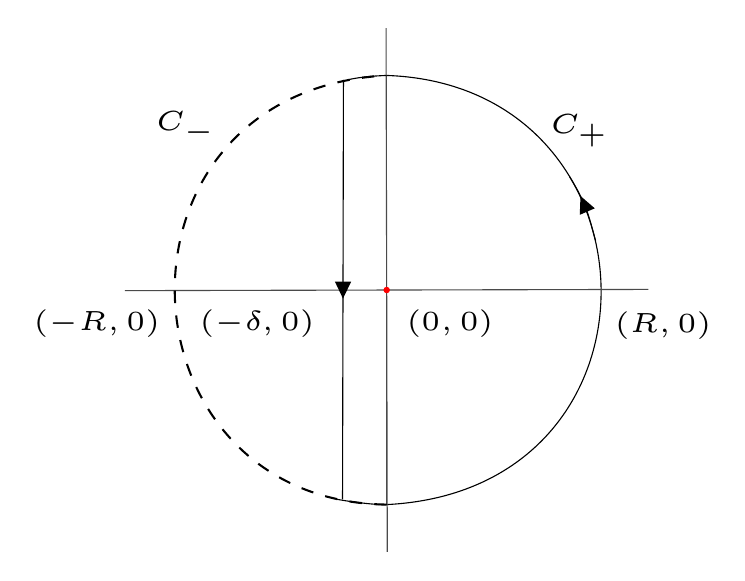
\begin{tikzpicture}[x=0.86pt,y=0.86pt,yscale=-1,xscale=1]
%uncomment if require: \path (0,357); %set diagram left start at 0, and has height of 357

%Curve Lines [id:da6356687025771366] 
\draw    (275.97,140.51) .. controls (393.49,144.53) and (398.68,314.72) .. (275.97,320.82) ;
%Straight Lines [id:da7778166164432772] 
\draw [color={rgb, 255:red, 74; green, 74; blue, 74 }  ,draw opacity=1 ]   (165.97,230.93) -- (385.97,230.41) ;
%Straight Lines [id:da7053132902182386] 
\draw [color={rgb, 255:red, 74; green, 74; blue, 74 }  ,draw opacity=1 ]   (276.23,340.67) -- (275.71,120.67) ;
%Straight Lines [id:da3860117988849814] 
\draw [color={rgb, 255:red, 74; green, 74; blue, 74 }  ,draw opacity=1 ]   (275.97,140.51) -- (275.97,320.82) ;
%Curve Lines [id:da8696519251258394] 
\draw [line width=0.75]  [dash pattern={on 4.5pt off 4.5pt}]  (275.97,320.82) .. controls (161.04,319.39) and (153.49,147.13) .. (275.97,140.51) ;
%Straight Lines [id:da885594660241974] 
\draw    (257.81,142.33) -- (257.42,318.61) ;
\draw [shift={(257.61,234.27)}, rotate = 270.13] [fill={rgb, 255:red, 0; green, 0; blue, 0 }  ][line width=0.08]  [draw opacity=0] (7.14,-3.43) -- (0,0) -- (7.14,3.43) -- cycle    ;
%Curve Lines [id:da01957205219237279] 
\draw    (260.05,142.23) .. controls (265.49,141.06) and (271.33,140.68) .. (275.97,140.51) ;
%Curve Lines [id:da7685319347743758] 
\draw    (275.97,320.82) .. controls (271.82,321.03) and (262.09,319.86) .. (255.08,318.61) ;
%Curve Lines [id:da9382254876031242] 
\draw    (352.85,183.1) .. controls (360.63,195.56) and (361.15,201.09) .. (363.74,209.91) ;
\draw [shift={(357.4,191.16)}, rotate = 66.46] [fill={rgb, 255:red, 0; green, 0; blue, 0 }  ][line width=0.08]  [draw opacity=0] (7.14,-3.43) -- (0,0) -- (7.14,3.43) -- cycle    ;
%Shape: Ellipse [id:dp016643737096258437] 
\draw  [color={rgb, 255:red, 255; green, 0; blue, 0 }  ,draw opacity=1 ][fill={rgb, 255:red, 255; green, 0; blue, 0 }  ,fill opacity=1 ] (274.86,230.67) .. controls (274.86,230.05) and (275.36,229.56) .. (275.97,229.56) .. controls (276.58,229.56) and (277.08,230.05) .. (277.08,230.67) .. controls (277.08,231.28) and (276.58,231.78) .. (275.97,231.78) .. controls (275.36,231.78) and (274.86,231.28) .. (274.86,230.67) -- cycle ;

% Text Node
\draw (125.36,236.93) node [anchor=north west][inner sep=0.75pt]  [font=\normalsize,xscale=2,yscale=2]  {\fontsize{4}{4}\selectfont$(-R,0)$};
% Text Node
\draw (282.08,236.93) node [anchor=north west][inner sep=0.75pt]  [font=\tiny,xscale=2,yscale=2] [align=left] {\fontsize{4}{4}\selectfont$( 0,0)$};
% Text Node
\draw (195.08,236.93) node [anchor=north west][inner sep=0.75pt]  [font=\tiny,xscale=2,yscale=2] [align=left] {\fontsize{4}{4}\selectfont$(-\delta,0)$};
% Text Node
\draw (369,236.93) node [anchor=north west][inner sep=1pt]  [font=\tiny,xscale=2,yscale=2]  {\fontsize{4}{4}\selectfont$(R,0)$};
% Text Node
\draw (342.5,154.9) node [anchor=north west][inner sep=0.75pt]  [font=\tiny,xscale=2,yscale=2]  {$\mathscr{C}_{+}$};
% Text Node
\draw (176.83,153.4) node [anchor=north west][inner sep=0.75pt]  [font=\tiny,xscale=2,yscale=2]  {$C_{-}$};

\end{tikzpicture}
    \end{center}

    donde $\delta>0$ (dependiendo de $R$) se escoge de tal forma que $g(s)$ es analítica en $\mathscr{C}$, esto se puede hacer ya que el conjunto $A:=\{(0,y): y\in [-R,R]\}$ es compacto y como $g(s)$ es analítica, $A$ se puede cubrir por bolas abiertas, en cada una de las cuales $g(s)$ es analítica, la compacidad permite escoger un subcubrimiento finito, del que obtenemos $\delta$.  Denotemos

    $$\mathscr{C}_+=\mathscr{C}\cap \{s:\sigma>0\},\quad \quad \mathscr{C}_-=\mathscr{C}\cap \{s:\sigma<0\}$$

    y como $C_-$ el semicírculo de radio $R$ a la izquierda de $\sigma=0$, el teorema de residuos de Cauchy nos da que \textcolor{red}{(cuando entienda bien la cuenta la escribo)}

    $$I_{\mathscr{C}}=\frac{1}{2\pi i}\int_{\mathscr{C}}\left(g(s)-g_T(s)\right)e^{sT}\left(1+\frac{s^2}{R^2}\right)\frac{1}{s}ds=g(0)-g_T(0).$$

    Sea $M = \sup _{t \geq 0}|f(t)|$. En $\mathscr{C}_{+}$, dado que $\sigma > 0$, tenemos

\[
\left|g(s)-g_T(s)\right| = \left|\int_T^{\infty} f(t) e^{-s t} d t\right| \leq M \int_T^{\infty} e^{-\sigma t} d t \ll \frac{e^{-\sigma T}}{\sigma}.
\]

Tomando $s = R e^{i \theta}$, entonces $R \cos \theta = \sigma$ en $\mathscr{C}_{+}$, obtenemos la siguiente estimación:

\begin{equation}
    \begin{aligned}
    \left|e^{s T} \frac{1}{s}\left(1+\frac{s^2}{R^2}\right)\right| &= e^{\sigma T}\left|\frac{1}{R e^{i \theta}}+\frac{e^{i \theta}}{R}\right|\\
    &=e^{\sigma T}\left|\frac{e^{-i\theta}+e^{i\theta}}{R}\right|\\
    &=e^{\sigma T}\left|\frac{2 \cos \theta}{R}\right| \ll e^{\sigma T} \frac{|\sigma|}{R^2},
\end{aligned}
\end{equation}

por lo tanto, acotando en la integral obtenemos que

\[
\left|I_{\mathscr{C}_{+}}\right| \ll \frac{1}{R^2}\left|\int_{\mathscr{C}_{+}} d s\right|=\frac{1}{R^2}\pi R\ll \frac{1}{R}.
\]

En $\mathscr{C}_{-}$, examinamos $g_T(s)$ y $g(s)$ por separado. Consideremos primero la integral

\[
I_1 := \frac{1}{2 \pi i} \int_{\mathscr{C}_{-}} g_T(s) e^{s T}\left(1+\frac{s^2}{R^2}\right) \frac{d s}{s}.
\]

Como $g_T(s)$ es entera y el resto del integrando es analítico a la izquierda de $\sigma = 0$, tenemos que

\[
I_1 = \frac{1}{2 \pi i} \int_{C_{-}} g_T(s) e^{s T}\left(1+\frac{s^2}{R^2}\right) \frac{d s}{s}.
\] 

Es decir, podemos integrar sobre el semicírculo \( C_{-} \) en lugar de \( \mathscr{C}_{-} \), con \( C_{-} \) orientado de la misma manera que \( \mathscr{C}_{-} \). Luego, observando que \( \sigma < 0 \) en este caso, tenemos  

\[
\left|g_T(s)\right| = \left|\int_0^T f(t) e^{-s t} d t\right| \leq M \int_0^T e^{-\sigma t} d t \ll \frac{e^{-\sigma T}}{|\sigma|}.
\]

La estimación en (3.1) sigue siendo válida, por lo que de manera análoga obtenemos que

$$|I_{1}|\ll \frac{1}{R},$$

nos queda acotar la integral restante

$$I_2=\frac{1}{2\pi i }\int_{\mathscr{C}_-}g(s)e^{st}\left(1+\frac{s^2}{R^2}\right)\frac{1}{s}ds.$$

Como $\mathscr{C}_-$ está contenido en un compacto en el que $g(s)$ es analítica, $|g(s)|$ se puede acotar por una constante que depende únicamente de $R$, digamos 

$$|g(s)|\leq M_R,$$

para todo $s \in \mathscr{C}_-$, $s=e^{i\theta}$ o $s=-\delta+it$, esto es, $s$ está en los arcos de circunferencia, o $s$ está en la recta vertical $\Re(s)=-\delta$, debemos acotar la intergral en estos dos caminos del contorno, para $s=e^{i\theta}$ ya tenemos una cota dada por (3.1), si $s=-\delta+it$ tenemos que

\begin{align*}
    \left|\frac{e^{s T}}{s}\left(1+\frac{s^2}{R^2}\right)\right|&\leq \frac{e^{-\delta T}}{|s|}\left(1+\frac{|s|^2}{R^2}\right)\\
    &\leq e^{-\delta T}\left(\frac{1}{|s|}+\frac{|s|}{R^2}\right)\\
    &\leq e^{-\delta T}\left(\frac{1}{\delta}+\frac{1}{R}\right)
,\end{align*}

ya que $|t|\leq R$, combinanto esta cota junto con (3.1) y sabiendo que $|g(s)|\leq M_R$, podemos acotar la integral como

$$|I_2|\ll \frac{M_R}{R^2}\left|\int_{\mathscr{C}_-} |\sigma|e^{\sigma T} d s\right|+\frac{R M_R e^{-\delta T}}{\delta}+M_R e^{-\delta T},$$


por lo tanto

\begin{equation}
    \begin{aligned}
    |g(0)-g_T(0)|&=|I_{\mathscr{C}}|\leq |I_{\mathscr{C}_+}|+|I_1|+|I_2|\\
    &\ll \frac{1}{R}+\frac{M_R}{R^2}\left|\int_{\mathscr{C}_-} |\sigma|e^{\sigma T} d s\right|+\frac{R M_R e^{-\delta T}}{\delta}+M_R e^{-\delta T}
.\end{aligned}
\end{equation}

En \( C_{-} \), tenemos \( \sigma < 0 \) y \( |\sigma| e^{\sigma T} \rightarrow 0 \) uniformemente en \( C_{-} \) cuando \( T \rightarrow \infty \). Por lo tanto, cuando \( T \rightarrow \infty \), el lado derecho de (3.2) converge a \( \dfrac{1}{R} \). Luego, tomando \( R \rightarrow \infty \), obtenemos 

\[
g(0) = \lim _{T \rightarrow \infty} g_T(0).
\]
\end{proof}

\begin{lemma}[Korevaar  y Zagier]

Sean $a_n\geq 0$ y $A(x)=\displaystyle\sum_{n\leq x} a_n$, si  la integral

$$\int_1^{\infty}\frac{A(x)-x}{x^2}dx$$

converge, entonces $A(x)\thicksim x$

\end{lemma}

\begin{proof}
    Supongamos que $A(x)\not\thicksim x$, entonces existe una constante $\lambda>1$ (o $\lambda<1$) tal que $A(x)\geq \lambda x$ (o $A(x)\leq \lambda x$) para infinitos valores de $x\to \infty$.\\

    Sin pérdida de generalidad consideramos el caso \( \lambda > 1 \). Dado que \( A(x) \) es una función creciente, se sigue que para cualquiera de los valores de \( x \) con \( A(x) \geq \lambda x \) y para \( x \leq t \leq \lambda x \), tenemos \( A(t) \geq A(x) \geq \lambda x \) y  

\[
\begin{aligned}
\int_x^{\lambda x} \frac{A(t)-t}{t^2} d t & \geq \int_x^{\lambda x} \frac{\lambda x-t}{t^2} d t = \int_1^\lambda \frac{\lambda x-v x}{(v x)^2} x d v \\
& = \int_1^\lambda \frac{\lambda-v}{v^2} d v\\
&=c(\lambda)
\end{aligned}
\]

que es una constante positiva que depende únicamente de \( \lambda \). Por lo tanto  

\[
\left|\int_x^{\infty} \frac{A(t)-t}{t^2} d t - \int_{\lambda x}^{\infty} \frac{A(t)-t}{t^2} d t\right| =c(\lambda),
\]

sin embargo, las integrales anteriores son colas de una integral convergente, por lo que ambas convergen a cero cuando \( x \rightarrow \infty \), esto contradice que $c(\lambda)>0$.\\
\end{proof}

Con esto ya podemos presentar una prueba del teorema de Wiener-Ikehara.\\

\begin{proof}\textit{ Teorema 3.1}. Tenemos, para $\Re(s)>1$ que
\[
F(s)=\sum_{n=1}^{\infty}a_nn^{-s} =s \int_1^{\infty}\frac{A(t)}{t^{s+1}} d t,
\]

Esto implica que en el semiplano \( \sigma > 1 \), \(\displaystyle \sum_{n=1}^{\infty} a_n n^{-s} \) converge absolutamente, \( F(s) \) es analítica y  

\[
F(s) - \frac{s}{s-1} = s \int_1^{\infty} \frac{A(t)-t}{t^{s+1}} d t.
\]

Cambiando \( s \) por \( s+1 \) y \( t = e^u \) en la integral, tenemos para \( \Re(s) > 0 \),  

\[
F(s+1) - 1 - \frac{1}{s} = (s+1) \int_0^{\infty} \frac{A\left(e^u\right) - e^u}{e^u} e^{-u s} d u.
\]

Por hipótesis \( A\left(e^u\right) = O\left(e^u\right) \), se sigue que la función \( f \) dada por  

\[
f(u) = \frac{A\left(e^u\right) - e^u}{e^u}
\]

es acotada en \( [0, \infty) \) e integrable en cada subintervalo cerrado y acotado de \( [0, \infty) \), y  

\begin{align}
    \frac{F(s+1) - 1 - \frac{1}{s}}{s+1} = \int_0^{\infty} f(u) e^{-s u} d u.
\end{align}

El lado izquierdo en (3.3) es analítico para \( \sigma > 0 \). Como \( F(s+1) \) tiene un polo simple en \( s = 0 \), vemos que

 \[ F(s+1) - \dfrac{1}{s}\]

 es analítica en \( s = 0 \), y para todo \( s \) con \( \sigma \geq 0 \). Por lo tanto, podemos aplicar el teorema 3.4 para obtener que la integral  

\[
\int_0^{\infty} \frac{A\left(e^u\right) - e^u}{e^u} d u = \int_1^{\infty} \frac{A(t)-t}{t^2} d t
\]

converge. Por el lema anterior, obtenemos que \( A(x) \sim x \).
\end{proof}

Con este teorema ya podemos obtener una prueba del TNP, sin embargo, en progresiones aritmética la serie de Dirichlet 

$$L(\chi,s)=\sum_{n=1}^{\infty} \frac{\chi(n)}{n^s}$$

no cumple la hipótesis $\chi(n)\geq 0$ del teorema de Wiener-Ikehara, también sabemos que el teorema de los números primos nos dice que

$$\pi(a,q,x)\thicksim \frac{x}{\varphi(q)\log  x},$$

por lo que esperamos aplicar el teorema de Wiener-Ikehara a una serie de Dirichlet con residuo $1/\phi(q)$, necesitamos extender el resultado para un conjunto más grande de series de Dirichlet, como mencionamos antes, haremos esto siguiendo a \cite{vatwani2015simple}, estas extensiones del teorema tauberiano son también tratadas en el texto de Ram Murty \cite{murty2007problems}

\begin{corollary}
    Sean $a_n \geq 0$ y $F(s)=\displaystyle\sum_{n=1}^{\infty} \frac{a_n}{n^s}$ una serie absolutamente convergente. Supongamos que se cumplen las siguientes condiciones:

\begin{itemize}
\item[a)] La función $F(s)$ se extiende a una función analítica en la región $\Re(s) \geq 1$ con un único polo simple en $s=1$, cuyo residuo es $R$.
\item[b)] $A(x)=\displaystyle \sum_{n \leq x} a_n=O(x)$.
\end{itemize}


Entonces, se tiene que

$$
A(x)=Rx+o(x) \text { cuando } x \rightarrow \infty \text {. }
$$
\end{corollary}

\begin{proof}
    Note que basta considerar $R> 0$, ya que si $R\leq 0$ basta probar el teorema para 

    $$F(s)+m\zeta(s)=\sum_{n=1}^{\infty} \frac{a_n+m}{n^s}$$

    con $m\in \Z$ tal que $m>|R|$. Para $R>0$ note que cambiando $a_n$ por $\dfrac{a_n}{R}$ y aplicando el teorema 3.1 obtenemos lo deseado.\\
\end{proof}

Finalizamos esta sección con el siguiente corolario

\begin{corollary}
Sea $
F(s) =\displaystyle \sum_{n=1}^{\infty} \frac{a_n}{n^s}
$ una serie de Dirichlet con coeficientes complejos. Sea $A(x)$ la suma parcial de los coeficientes. Supongamos que existe una serie de Dirichlet $
G(s) = \displaystyle\sum_{n=1}^{\infty} \frac{b_n}{n^s}
$ con coeficientes no negativos, tal que:  

\begin{itemize}
    \item[(a)] $\left|a_n\right| \leq b_n$ para todo $n\in \N$.
    \item[(b)] $G(s)$ es absolutamente convergente para $\Re(s) > 1$.
    \item[(c)] La función $G(s)$ (respectivamente $F(s)$) tiene una extensión analítica en la región $\Re(s) \geq 1$, sin polos excepto por un polo simple en $s = 1$ con residuo $R$ (respectivamente $r$).
    \item[(d)] $B(x):=\displaystyle\sum_{n \leq x}b_n=O(x)$.
\end{itemize}

Entonces, cuando $x \rightarrow \infty$, $
A(x) = r x + o(x).
$
\end{corollary}


\begin{proof}
Si los coeficientes $a_n$ son reales, consideramos la serie $G(s)-F(s)$, que tiene coeficientes no negativos y satisface las condiciones del corolario anterior, obteniendo

$$
\sum_{n \leq x}\left(b_n-a_n\right) = (R-r) x + o(x)
$$

cuando $x \to \infty$. Dado que $B(x) = R x + o(x)$, esto prueba el resultado en el caso de coeficientes reales.  

Si los coeficientes $a_n$ no son reales, definimos

$$
F^*(s) = \sum_{n=1}^{\infty} \frac{\overline{a_n}}{n^s},
$$

de modo que

$$
F = \frac{F + F^*}{2} + i\left(\frac{F - F^*}{2 i}\right),
$$

y aplicamos el resultado para coeficientes reales separadamente a la parte real e imaginaria de la expresión anterior.
\end{proof}


\section{Prueba del teorema de los números primos}

Para probar el TNP queremos ver que $\psi(x)\thicksim x$, en este punto, el camino a seguir es claro, necesitamos probar que la serie de Dirichlet de la función de Von Mangolth cumple las condiciones del teorema de Wiener-Ikehara.\\

Primero vamos a verificar que en efecto $\psi(x)=O(x)$, en el capítulo de premilinares vimos que $\psi(x)-\vartheta(x)=O(\sqrt{x}\log^2 x)$, por lo tanto, basta ver que en efecto $\vartheta(x)=O(x)$. Dado $n\in \N$, note que

$$2^{2n}=(1+1)^{2n}=\binom{2n}{0}+\ldots+\binom{2n}{2n}\geq \binom{2n}{n},$$

todo número primo $n<p<2n$ divide a $(2n)!$ y no a $(n!)^2$, de lo que obtenemos

$$2^{2n}=(1+1)^{2n}=\binom{2n}{0}+\ldots+\binom{2n}{2n}\geq \binom{2n}{n}\geq \prod_{n<p<2n}p=e^{\displaystyle\vartheta(2n)-\vartheta(n)},$$

tomando el logaritmo en los extremos, se sigue que $2n\log 2\geq \vartheta(2n)-\vartheta(n)$, podemos reescribrir esto como

$$\vartheta(x)-\vartheta\left(\frac{x}{2}\right)\leq x\log 2,
$$

entonces

\begin{equation}
    \begin{aligned}
 \vartheta(x)-\vartheta\left(\frac{x}{2}\right) &\leq x\log2, \\
 \vartheta\left(\frac{x}{2}\right) -\vartheta\left(\frac{x}{4}\right) &\leq \frac{x}{2}\log2,\\
 &\hspace*{0.191cm}\vdots \\
 \vartheta\left(\frac{x}{2^r}\right)-0 &\leq \frac{x}{2^r}\log 2,
\end{aligned}
\end{equation}

donde $r$ es el mayor entero tal que $x>2^r$, sumando las desigualdades en (3.4), obtenemos que

\begin{align*}
    \vartheta(x)&\leq x\log 2\left(\sum_{i=0}^{r} \frac{1}{2^{i}}\right)\leq x\log(4)\left(1-\frac{1}{2^{r+1}}\right)\leq x\log 4
,\end{align*}

con lo que hemos probado que $\vartheta(x)=O(x)$.\\

\begin{theorem}[Principio del argumento]
    Sea $f(z)$ una función analítica, 

    \begin{itemize}
        \item[$\bullet$]si $z_0$ es un polo de $f(z)$ de orden $m$, entonces $z_0$ es un polo simple de $\dfrac{f^{\prime}(z)}{f(z)}$ con residuo $-m$,

        \item si $z_0$ es un cero de $f(z)$ de orden $m$, entonces $z_0$ es un polo simple de $\dfrac{f^{\prime}(z)}{f(z)}$ con residuo $m$.
    \end{itemize}
\end{theorem}

\begin{proof}
    Sea $z_0$ un cero de $f$. Podemos escribir 

$$
f(z) = \left(z - z_0\right)^m g(z),
$$

donde $m$ es la multiplicidad del cero y por lo tanto $g\left(z_0\right) \neq 0$, tenemos que

$$
f^{\prime}(z) = m\left(z - z_0\right)^{m-1} g(z) + \left(z - z_0\right)^m g^{\prime}(z),
$$

y

$$
\frac{f^{\prime}(z)}{f(z)} = \frac{m}{z - z_0} + \frac{g^{\prime}(z)}{g(z)}.
$$

Dado que $g\left(z_0\right) \neq 0$, se sigue que $\dfrac{g^{\prime}(z)}{g(z)}$ no tiene singularidades en $z_0$, por lo tanto es analítica en $z_0$. Esto implica que el residuo de $\dfrac{f^{\prime}(z)}{f(z)}$ en $z_0$ es $m$.\\

Análogamente, si $z_{0}$ es un polo de $f$, 

$$
f(z)=(z-z_{0})^{-m}h(z),
$$
donde $m$ es el orden del polo, y $h\left(z_0\right) \neq 0$. Entonces, 
$$
f^{\prime}(z) = -m\left(z - z_0\right)^{-m-1} h(z) + \left(z - z_0\right)^{-m} h^{\prime}(z),
$$
y
$$
\frac{f^{\prime}(z)}{f(z)} = \frac{-m}{z - z_0} + \frac{h^{\prime}(z)}{h(z)}.
$$
\end{proof}

Recordemos que

$$F(s)=\sum_{n=1}^{\infty} \frac{\Lambda(n)}{n^s}=-\frac{\zeta^{\prime}(s)}{\zeta(s)}
,$$
converge absolutamente en $\Re(s)>1$ (corolario 1.30), entonces el principio del argumento nos dice que $F(s)$ tiene un polo simple en $s=1$ con residuo 1, dado por el polo que tiene $\zeta(s)$ en $s=1$.\\

Para garantizar que $F(s)$ tiene una extensión analítica a $\Re(s)\geq 1$, excepto por un \textbf{único} polo simple en $s=1$ con residuo 1, debemos ver que $\zeta(s)\neq 0$ en la recta $\Re(s)=1$, este hecho junto con el teorema de Wiener-Ikehara implican inmediatamente el teorema de los números primos.

\begin{lemma}
    Si $\theta\in \mathbb{R}$, entonces $3+4\cos\theta+\cos2\theta\geq 0$
\end{lemma}

\begin{proof}
    En efecto
    \begin{align*}
        0&\leq 2(1+\cos\theta)^2\\
        &=2(1+2\cos\theta+\cos^2\theta)\\
        &=2+4\cos\theta+1+\cos(2\theta)
    .\end{align*}
    \end{proof}

\begin{theorem}
$\zeta(1+it)\neq 0$ para todo $t\neq 0$.
\end{theorem}

\begin{proof}
Note que
    \begin{align*}
        p^{-n\sigma}\cos(nt\log p)&=p^{-n\sigma}\cos(-nt\log p)\\
        &=p^{-n\sigma}\Re(exp(i\log p^{-nt}))\\
        &=\Re(p^{-n\sigma}p^{-int})\\
        &=\Re(p^{-ns})
    ,\end{align*}

por lo tanto

\begin{align*}
    \Re(\log\zeta(s))&=\sum_{p}\sum_{n=1}^{\infty} \frac{\Re(p^{-ns})}{n}\\
    &=\sum_{p}\sum_{n=1}^{\infty} \frac{p^{-n\sigma}}{n}\cos(nt\log p)
.\end{align*}

Ahora, como $\Re(\log z)=\log|z|$, entonces por el lema 3.9

\begin{align*}
    0&\leq \sum_p \sum_{n=1}^{\infty}\frac{p^{-n \sigma}}{n}(3+4 \cos (n t \log p)+\cos (2 n t \log p))\\
     &=\Re(3\log\zeta(\sigma)+4\log\zeta(\sigma+it)+\log\zeta(\sigma+2it))\\
    &=3 \log |\zeta(\sigma)|+4 \log |\zeta(\sigma+i t)|+\log |\zeta(\sigma+2 i t)|
,\end{align*}

esto es

$$
|\zeta(\sigma)|^3|\zeta(\sigma+i t)|^4|\zeta(\sigma+2 i t)| \geqslant 1,
$$

obtenemos la identidad

\begin{equation}
    |(\sigma-1) \zeta(\sigma)|^3\left|\frac{\zeta(\sigma+i t)}{\sigma-1}\right|^4|\zeta(\sigma+2 i t)| \geqslant \frac{1}{\sigma-1} .
\end{equation}

Supongamos que $\zeta(1+it)=0$ para algún $t\neq 0$, entonces

$$\lim_{\sigma \to 1}\frac{\zeta(\sigma+it)-\zeta(1+it)}{\sigma-1}=\lim_{\sigma \to 1}\frac{\zeta(\sigma+it)}{\sigma-1}=\zeta^{\prime}(1+it),$$

como $\zeta(s)$ tiene un polo simple en $s=1$, se sigue que

$$\lim_{\sigma \to 1} (\sigma-1)\zeta(\sigma)=1,$$

esto muestra que 

$$\lim _{\sigma \rightarrow 1}|(\sigma-1) \zeta(\sigma)|^3\left|\frac{\zeta(\sigma+i t)}{\sigma-1}\right|^4|\zeta(\sigma+2 i t)|$$

existe y es igual a $\left|\zeta^{\prime}(1+i t)\right|^4|\zeta(1+2 i t)|$, lo que contradice (3.5).
\end{proof}

\begin{corollary}[Teorema de los números primos]
$$\pi(x)\thicksim \frac{x}{\log x},\quad \psi(x)\thicksim x.$$
\end{corollary}

\begin{proof}
    Sea $F(s)=\displaystyle\sum_{n=1}^{\infty} \dfrac{\Lambda(n)}{n^s}$, como $F(s)$ tiene un único polo simple en $s=1$ con residuo $1$, aplicando el teorema de Wiener-Ikehara se sigue que

    $$\psi(x)=\sum_{n\leq x} \Lambda(n)=x+o(x),$$

    esto es

    $$\lim_{n \to \infty} \frac{\psi(x)}{x}=\lim_{n \to \infty} \frac{x+o(x)}{x}=1.$$
\end{proof}

\begin{note}
Una aplicación elemental de la regla de L´Hopital es la siguiente:

\begin{align*}
    \displaystyle\lim_{x \to \infty} \frac{\displaystyle\int_2^x \displaystyle\frac{1}{\log t}dt}{\displaystyle\frac{x}{\log x}}=\lim_{x \to \infty} \frac{\displaystyle\frac{1}{\log x}}{\displaystyle\frac{\log x-x^{-1}}{\log^2x}}=\lim_{x \to \infty} \frac{1}{1-(x\log x)^{-1}}=1
.\end{align*}

Esta presentación del teorema de los números primos, a saber,

$$\pi(x)\thicksim \int_2^x\frac{1}{\log t}dt,$$

nos dice que integral la densidad de los primos nos da el números de primos menores que x.
\end{note}
\blankpages
\chapter{Primos en progresiones aritmética}
%!TEX root = ../main.tex

\thispagestyle{empty}
\vspace{-0.5cm}

\cleanchapterquote{Los encantos de esta ciencia sublime, las matemáticas, solo se le revelan a aquellos que tienen el valor de profundizar en ella.}{Carl Friedrich Gauss}{}

El teorema de Dirichlet nos dice que hay infinitos primos de la forma $a,a+n , a+2n,\ldots$ siempre que $(a,n)=1$, este es un resultado importante en teoría de números sin embargo podemos decir mucho más sobre primos en progresiones aritmética. Hemos probado el teorema de los números primos en el capítulo anterior y una pregunta natural es cómo se extiende este a progresiones aritmética, por ejemplo, si estudiamos los primos de la forma $4k+1$ y $4k+3$, ¿hay la misma cantidad de primos de la forma $4k+1$ que $4k+3$?, ¿podemos esperar una distribución uniforme de estos?, la respuesta nos la dará el TNP, este nos dice que

$$\pi(1,4,x)\thicksim \frac{x}{\varphi(4)\log x}=\frac{x}{2\log x},\quad \pi(3,4,x)\thicksim \frac{x}{2\log x}.$$

Más precisamente $(\Z/4\Z)^\times=\{\overline{1},\overline{3}\}$, tenemos dos clases generadoras de primos y en cada una tenemos la mitad, este resultado no es un hecho trivial, por mucho tiempo los matemáticos pensaron que este no era el caso, la evidencia heurística apuntaba a que habían más primos de la forma $4k+3$ hasta que Littlewood demostró que $\pi(3,4,x)-\pi(1,4,x)$ tiene infinitos cambios de signo, estos temas se abordan de manera más detallada en \cite{granville2006prime}.
\section{Teorema de los números primos en progresiones aritmética}

Como antes, la idea es aplicar el teorema de Wiener-Ikehara para probar el TNP, por lo que presentamos antes este teorema sobre no nulidad de $L-$funciones, análogo al que tenemos para $\zeta(s)$

\begin{theorem}
    Sea $\chi$ un carácter de Dirichlet, entonces

    $$L(\chi,s)\neq 0, \text{ si }\Re(s)>1$$
\end{theorem}

\begin{proof}
    Como $\Re(s)>1$, entonces

    $$L(\chi,s)=\prod_p\frac{1}{1-\chi(p)p^{-s}},$$

    de manera análoga al teorema 1.38, el término $\dfrac{1}{1-\chi(p)p^{-s}}=\dfrac{p^s}{p^s-\chi(p)}\neq 0$ para todo $p$, esto nos  da que el producto no tiene factores nulos y por tanto no converge a 0.
\end{proof}

\begin{theorem}[Teorema de los números primos en progresiones aritmética]
Dados $a$ y $m$ primos relativos.
    $$\pi(a,m,x)\thicksim \frac{x}{\varphi(m)\log x}$$    
\end{theorem}

Observemos lo siguiente, si $h$ es una función aritmética completamente multiplicativa

\begin{align*}
    ((f*g)h)(n)&=\sum_{j\mid n}f(j)g\left(\frac{n}{j}\right)h(n)=\sum_{j\mid n}f(j)g\left(\frac{n}{j}\right)h\left(j\right)h\left(\frac{n}{j}\right)\\
    &=\sum_{j\mid n}f(j)h\left(j\right)g\left(\frac{n}{j}\right)h\left(\frac{n}{j}\right)\\
    &=\sum_{j\mid n}fh(j)gh\left(\frac{n}{j}\right)\\
    &=(fh*gh)(n)
.\end{align*}

Podemos aplicar esto para obtener una fórmula para la derivada logarítmica de la función $L(\chi,s)$

\begin{align*}
    -L^{\prime}(\chi,s)&=\sum_{n=1}^{\infty} \frac{\chi(n)\log(n)}{n^s}=\sum_{n=1}^{\infty} \frac{\chi(n)(\Lambda*1)(n)}{n^s}=\sum_{n=1}^{\infty} \frac{(\chi\Lambda*1\chi)(n) }{n^s}\\
    &=\sum_{n=1}^{\infty} \frac{\chi(n)\Lambda(n)}{n^s}\sum_{n=1}^{\infty} \frac{\chi(n)}{n^s},
\end{align*}

esto es

$$\boxed{-\frac{L^{\prime}}{L}(\chi,s)=\sum_{n=1}^{\infty} \frac{\chi(n)\Lambda(n)}{n^s}}.$$

Obtendremos el TNP en progresiones aritmética de aplicar el teorema de Wiener Ikehara a la función

$$F(s)=\sum_{n\equiv a \bmod{m}}\frac{\Lambda(n)}{n^s},$$

pero para esto debemos primero ver qué forma tiene esta función, sea $f(n)$ la función característica de la progresión, usando su representación de Fourier obtenemos que

\begin{align*}
    F(s)&=\sum_{n=1}^{\infty}\frac{\Lambda(n)f(n)}{n^s}=\sum_{n=1}^{\infty} \frac{\Lambda(n)}{n^s}\left(\frac{1}{\varphi(m)}\sum_\chi \chi(a^{-1})\chi(n)\right)\\
    &=\frac{1}{\varphi(m)}\sum_\chi\chi(a^{-1})\left(\sum_{n=1}^{\infty} \frac{\chi(n)\Lambda(n)}{n^s}\right)\\
    &=\frac{1}{\varphi(m)}\sum_\chi\chi(a^{-1})\left(-\frac{L^{\prime}}{L}(\chi,s)\right)
.\end{align*}

Sabemos que todas estas $L-$funciones presentes en la suma son analíticas en $\Re(s)\geq 1$ excepto $L(\chi_0,s)$ que tiene un polo simple en $s=1$ dado por el polo simple que tiene $\zeta(s)$, aplicando el principio del argumento y suponiendo que ninguna de estas $L$ funciones se anula en la recta vertical $\Re(s)=1$ sabremos que en la suma anterior el único carácter que contribuye un polo es el trivial, este polo tendrá residuo $1$, luego la función $F(s)$ cumple todas las condiciones del teorema de Wiener Ikehara y además tiene residuo $\dfrac{1}{\varphi(m)}$, esto es

$$\psi(a,m,x)=\sum_{\substack{n\leq x\\n\equiv a\bmod{m}}}\Lambda(n)\thicksim \frac{x}{\varphi(m)}.$$

Repasando lo anterior, las derivadas logarítmicas son todas analíticas en $\Re(s)\geq 1$ por el principio del argumento, solo una tiene un polo en $s=1$, la del carácter trivial y esta nos da el residuo que esperamos. El teorema de los números primos es una consecuencia inmediata de la siguiente afirmación
\begin{theorem}
    Sea $\chi$ un carácter de Dirichlet, $L(\chi,1+it)\neq 0$  para todo $t$
\end{theorem}

La prueba de este teorema no es sencilla, recordemos que para $\zeta(s)$ no lo fue, requería de ciertas estimaciones que no son evidentes, en general estudiar las regiones de no nulidad de $L-$funciones es un problema profundo en teoría analítica de números que además permanece abierto. La prueba que veremos aquí es la propuesta en \cite{murty2007problems}.

\subsection{La no nulidad de \texorpdfstring{$L(1+it,\chi)$ }{Lg}}

Como en el capítulo anterior, probar esta no nulidad requiere de identidades trigonométricas, ya que al tomarle parte real a una serie de Dirichlet nos aparecen cosenos de manera natural, sin embargo, cuando vimos que $L(1,\chi)\neq 0$ para $\chi\neq\chi_0$ consideramos un producto de $L-$funciones y realizamos un argumento de conteo de ceros y polos. En este caso también vamos a considerar el producto de todas las $L$-funciones, veremos que

$$f(s)=\prod_\chi L(s,\chi)$$ 

no se anula en la recta vertical $\Re(s)=1$ y por lo tanto ninguna $L-$función, para esto aplicaremos un argumento que proviene de Landau y que es modificado en \cite{murty2007problems}, el estudio de las series de Dirichlet con coeficientes no negativos, por lo que estudiaremos la expresión $\log(f(s))$.\\

 Finalmente, como estamos trabajando con $\log(f(s))$, el logaritmo transforma este producto de $L-$funciones en una suma y vamos a necesitar identidades sobre suma de cosenos, particularmente la identidad de Lagrange para el núcleo de Dirichlet.

 \begin{theorem}
Para $0 < \theta < 2\pi$.
     \[
    \frac{1}{2} + \cos \theta + \cos(2\theta) + \dots + \cos(n\theta) = \frac{\sin\left((n + \frac{1}{2})\theta\right)}{2 \sin\left(\frac{\theta}{2}\right)},
    \]
 \end{theorem}

 \begin{proof}
     Note que si tomamos $|z|=1$ con $z\neq 1$, entonces $z=exp(i\theta)$, de esto se sigue que

    $$\Re\left(\sum_{k=0}^{n} z^k\right)=\sum_{k=0}^{n} \Re(z^k)=\sum_{k=0}^{n}cos(k\theta).$$

    En efecto
    \begin{align*}
      \Re\left(\sum_{k=0}^{n} z^k\right)&=\Re\left(\frac{z^{n+1}-1}{z-1}\right)\\
      &=\Re\left(\frac{exp\left(i(n+1)\theta)\right) -1}{exp(i\theta)-1}\right)\\
      &=\Re\left(\frac{exp(i(n+1)\theta/2)}{exp(i\theta/2)}\frac{exp(-i(n+1)\theta/2)-exp(i(n+1)\theta/2)}{exp(-i\theta/2)-exp(i\theta/2)}\right)
    .\end{align*}

   Note que el último término de la derecha  de puede escribir como

   $$\Re\left(exp(in\theta/2)\frac{\sin\left((n+1)\theta/2\right)}{\sin(\theta/2)}\right)=\cos(n\theta/2)\frac{\sin((n+1)\theta/2)}{\sin(\theta/2)},$$

   además
   
   $$
\begin{aligned}
\cos \left(\frac{n \theta}{2}\right) \sin \left(\frac{(n+1) \theta}{2}\right)&=\frac{1}{2}\left(\sin \left(\frac{\theta n}{2}+\frac{\theta(n+1)}{2}\right)+\sin \left(\frac{\theta(n+1)}{2}-\frac{n \theta}{2}\right)\right. \\
& =\frac{1}{2}\left(\sin \left(\frac{\theta(2 n+1)}{2}\right)+\sin \left(\frac{\theta}{2}\right)\right) \\
& =\frac{1}{2} \sin \left(\theta\left(n+\frac{1}{2}\right)\right)+\frac{1}{2} \sin \left(\frac{\theta}{2}\right),
\end{aligned}
$$
dividiendo entre $\sin\left(\displaystyle\frac{\theta}{2}\right)$ obtenemos que

\[
    1 + \cos \theta + \cos(2\theta) + \dots + \cos(n\theta) = \frac{1}{2} + \frac{\sin\left((n + \frac{1}{2})\theta\right)}{2 \sin\left(\frac{\theta}{2}\right)},
    \]

de lo que se sigue el resultado.
 \end{proof}

 \begin{lemma}
$$1+\frac{\sin 3 \theta}{\sin \theta}+\frac{\sin 5 \theta}{\sin \theta}+\cdots+\frac{\sin (2 n-1) \theta}{\sin \theta}=\left(\frac{\sin n \theta}{\sin \theta}\right)^2$$
 \end{lemma}

Omitimos la prueba aquí ya que el resultado se sigue por inducción y se puede consultar en \cite{murty2007problems}.

 \begin{theorem}
     Para todo entero $m\geq 0$,

     $$(2 m+1)+2 \sum_{j=0}^{2 m-1}(j+1) \cos (2 m-j) \theta=\left(\frac{\sin \left(m+\frac{1}{2}\right) \theta}{\sin \frac{\theta}{2}}\right)^2.$$
 \end{theorem}

 \begin{proof}
     Cambiando el orden de sumación, podemos reescribir la identidad como  sigue 

     $$2 m+1+2 \sum_{j=1}^{2 m}(2 m-j+1) \cos j \theta=\left(\frac{\sin \left(m+\frac{1}{2}\right) \theta}{\sin \frac{\theta}{2}}\right)^2 .$$

     Tomando $\theta=2\varphi$, debemos probar que

     $$2 m+1+2 \sum_{j=1}^{2 m}(2 m-j+1) \cos 2 j \varphi=\left(\frac{\sin (2 m+1) \varphi}{\sin \varphi}\right)^2,$$

     por el teorema 4.4

     $$1+2 \sum_{j=1}^n \cos 2 j \varphi=\frac{\sin (2 n+1) \varphi}{\sin \varphi}.$$

     Ahora note que 

     \begin{align*}
         \sum_{n=0}^{2m}(1+2 \sum_{j=1}^n \cos 2 j \varphi)&=(2m+1)+2 \sum_{n=0}^{2m}\sum_{j=1}^n \cos 2 j \varphi\\
         &=\sum_{n=0}^{2m}\frac{\sin (2 n+1) \varphi}{\sin \varphi}
     .\end{align*}

     De esto se sigue que,

     \begin{align*}
         (2m+1)+2 \sum_{n=0}^{2m}\sum_{j=1}^n \cos 2 j \varphi&=(2 m+1)+2 \sum_{j=1}^{2 m} \cos 2 j \varphi \sum_{j \leq n \leq 2 m} 1\\
         &=(2 m+1)+2 \sum_{j=1}^{2 m}(2 m-j+1) \cos 2 j \varphi\\
         &=\sum_{n=0}^{2 m} \frac{\sin (2 n+1) \varphi}{\sin \varphi}\\
         &=\left(\frac{\sin (2 m+1) \varphi}{\sin \varphi}\right)^2
     .\end{align*}
 \end{proof}

\begin{theorem}[K. Murty]
Sea $f(s)$ una función a valor complejo que satisface las siguientes condiciones

\begin{itemize}
    \item[$\bullet$] $f$ es holomorfica y no nula en $\Re(s)>1$,
    \item[$\bullet$] $\log f(s)$ se puede escribir como una serie de Dirichlet
    $$
    \sum_{n=1}^{\infty} \frac{b_n}{n^s}
    $$
    con $b_n \geq 0$ para $\Re(s)>1$;
    \item[$\bullet$] en la recta $\Re(s)=1, f$ es holomorfica excepto por un polo de orden $e \geq 0$ en $s=1$.
\end{itemize} 

Si $f$ tiene un cero en $\Re(s)=1$, entonces el orden del cero está acotado por $e/2$.
\end{theorem}

\begin{proof}
    Supongamos que $f$ tiene un cero en $1+it_0$ de orden $k>e/2$,entonces $e\leq2k-1$, considere la función

    $$\begin{aligned}
g(s) & =f(s)^{2 k+1} \prod_{j=1}^{2 k} f\left(s+i j t_0\right)^{2(2 k+1-j)} \\
& =f(s)^{2 k+1} f\left(s+i t_0\right)^{4 k} f\left(s+2 i t_0\right)^{4 k-2} \cdots f\left(s+2 k i t_0\right)^2,
\end{aligned}$$
entonces $g(s)$ es holomorfica en $\Re(s)>1$ y tiene un cero de al menos orden 1 en $s=1$ ya que 
$$
4 k^2-(2 k+1) e \geq 4 k^2-(2 k+1)(2 k-1)=1
$$

donde $k$ es el orden del cero y $e$ el orden del polo. Por otro lado, para $\Re(s)>1$,

$$
\log g(s)=\sum_{n=1}^{\infty} \frac{b_n}{n^s}\left(2 k+1+2 \sum_{j=1}^{2 n} 2(2 k+1-j) n^{-i j t_0}\right) .
$$

Sea $\theta=t_0 \log n$. Entonces para $s=\sigma>1$,
$$\Re (\log g(\sigma))=\log |g(\sigma)|=\sum_{n=1}^{\infty} \frac{b_n}{n^\sigma}\left(2 k+1+\sum_{j=1}^{2 k} 2(2 k+1-j) \cos j \theta\right),$$
por el teorema anterior, el término del paréntesis es no negativo, de esto se sigue que $|g(\sigma)|\geq 1$, una contradicción ya que cuando $\sigma\to 1$, $g(s)=0$.
\end{proof}

\begin{theorem}
    $L(s,\chi)\neq 0$ para todo $s$ con $\Re(s)=1$.
\end{theorem}

\begin{proof}
    Sea $f(s)=\prod_\chi L(s,\chi)$ con $\chi$ un carácter de Dirichlet módulo $q$, claramente $f(s)$ es holomorfica y no nula en $\Re(s)>1$, además

    $$\log f(s)=\sum_\chi \log L(s, \chi)=\sum_{n, p} \frac{1}{n p^{n s}} \sum_\chi \chi\left(p^n\right).$$

    Note que 

    \begin{align*}
        f(p^n)=\begin{cases}
        1 &\text{ si }p^n\equiv 1 \bmod{q}\\
        0 &\text{ e.o.c.}
    \end{cases}&=\frac{1}{\varphi(q)}\sum_\chi \chi(p^n)\overline{\chi(1)}\\
    &=\frac{1}{\varphi(q)}\sum_\chi \chi(p^n)
    ,\end{align*}

    de esto se sigue que 

    $$\log(f(s))=\varphi(q) \sum_{\substack{n, p \\ p^n \equiv 1(\bmod q)}} \frac{1}{n p^{n s}},$$

    luego $\log(f(s))$ es una serie de Dirichlet con coeficientes no negativos. En la recta $\Re(s)=1$, $f$ es holomorfica excepto por un polo simple en $s=1$, a saber $L(1,\chi_0)$. Por el teorema 4.7, si $f(s)$ tiene un cero  en $\Re(s)=1$ entonces el orden del cero está acotado por $1/2$, esto es que $f(s)$ no se anula en $\Re(s)=1$ y por lo tanto $L(s,\chi)$.
\end{proof}

\begin{corollary}
    Dados $a$ y $q$ primos relativos,

    $$\psi(a,q,x)\thicksim \frac{x}{\varphi(q)}.$$
\end{corollary}

Como en el teorema de los números primos, es posible obtener mejores cotas para el error estudiando regiones donde $L(s,\chi)\neq 0$

\begin{theorem}[Siegel–Walfisz]
Dados $N\in \R$ y $(a,q)=1$, existe $C_N$ tal que

$$\psi(a, q, x)=\frac{x}{\varphi(q)}+O\left(x \exp \left(-C_N(\log x)^{\frac{1}{2}}\right)\right)$$

si $q \leq(\log x)^N .$
\end{theorem}

Sin embargo es algo que va más allá de los límites de este, ya muy largo trabajo.
%%%%%%%%%%%%%%%%%%%%%%%%%%%%%%%%%%%%%%%%%%%%%%%%%%%%%%%%%%%
%%                BIBLIOGRAFÍA                           %%   
%%%%%%%%%%%%%%%%%%%%%%%%%%%%%%%%%%%%%%%%%%%%%%%%%%%%%%%%%%%
\nocite{*}
\blankpages
\bibliographystyle{unsrt}
\bibliography{references}



\end{document}